% \subsection{Case studies}\label{ss:cases}

% \subsubsection{URL denylisting}
\label{ss:url}
\begin{figure}[h!]
% \vspace{-0.2 cm}
\begin{minipage}{\linewidth}
\begin{lstlisting}[language=C++, caption={
Relevant function of the setup protocol of the URL denylisting application with bridging.
},
style=mystyle, 
label=list:pmt_sort,
xleftmargin=0.45cm,
% xrightmargin=-0.12\linewidth,
% linewidth=0.88\linewidth
]
template <int S> vector<SecureMod>
sort (int logt, vector<int> filter,
  const vector<SecureUint<S>> & order)
{
  using SecUint = SecureUint<S>;
  auto s = order.size();
  auto n = SecureMod::slots();
  auto nsp = n*s*logt;
  filter.resize(nsp, 0);
  vector<vector<unsigned>> f;
  for (int i=0; i<s; i++)
  {
    vector<unsigned> poly;
    for (int j=0; j<n; j++)
    {
      unsigned plain = 0;
      for (int k=0; k<logt; k++)
        plain = (plain<<1) +
          bool( filter[i+(j*logt+k)*s] );
      poly.push_back(plain);
    }
    f.push_back(poly);
  }
  
  $//$vector<SecUint> efilter;
  vector<SecureMod> efilter;
  for ( int i=0; i<s; i++ )
  {
    const auto & c = order[i];
    $//$vector<SecUint> partial_res;
    vector<SecureMod> partial_res;
    for (int j=0; j<s; j++)
    {
      $//$auto tmp = (c==j) * SecUint(f[j]);
      auto tmp = SecureMod(c==j) * f[j];
      partial_res.push_back(tmp);
    }
    $//$ low depth array summation  
    auto r = sum(partial_res);
    efilter.push_back(r);
  }
  return efilter;
}
\end{lstlisting}
\end{minipage}
\vspace{-0.6 cm}
% \vspace{-0.1 cm}
\end{figure}

We evaluate the performance improvements provided by bridging using a URL denylisting application as a case study \cite{urldenylist}.
The application implements a Private Membership Test (PMT) protocol, a common cryptographic building block for privacy-preserving applications.
Its main operation is checking if an element is part of a database without revealing information about the element.
In this scenario, the server hosting the database is semi-trusted (honest-but-curious).

URL denylisting is the process where a URL is being checked against a known database of malicious URLs; if there is a match, the access to the website is blocked. URL denylisting can be used in conjunction with URL rewriting to protect against e-mail phishing attacks. In other words, when an email comes to the company server, its URLs are being replaced by a redirection to the service provider site, which checks whether the link is malicious or not. If it is benign, the user is automatically forwarded to the webpage. While this (supposedly) protects against phishing attacks, it introduces a huge privacy problem, since the company hosting the service can clearly see which links the users are visiting, and can potentially sell the data to other parties. 

The PMT protocol we evaluate here is composed of two main phases: setup and query. In the setup phase, the database is converted into a format that enables fast queries. The query phase is simply checking if a particular element is part of the database.
While queries are fast, the setup is expensive since it uses comparison operations. As mentioned in the previous sections, comparisons require bit-level arithmetic, leading to execution times of more than a day for databases with millions of entries. Implementing a faster setup protocol is therefore critical to the practicality of the application. 

The setup protocol is composed of three main stages: 1) The server database containing the list of malicious URLs is converted into a Bloom filter \cite{bloomfilter}. The server then informs the size of this Bloom filter $m$ to the client. 2) In the next step, the client creates a list with random permutations of \mbox{$\ceil{ {m}/({n \cdot \floor{\log_{2}{t}}} ) }$} unique integers, where $m$ is the size of the Bloom filter, $n$ is the polynomial degree, and $t$ is the plaintext modulus. The client encrypts the list with its public key and sends to the server. 3) Finally, the server runs a particular homomorphic algorithm that sorts the Bloom filter into a way only known to the client. This produces an encrypted Bloom filter in this particular order.

Out of the three stages in the setup, only the third one operates homomorphically on encrypted data. Therefore, we implemented the third stage of the setup protocol using bridging and compared its performance against the bit-level arithmetic implementation.
As shown in Fig. \ref{fig:application}, bridging provides approximately one order of magnitude of performance improvement for this application, reducing the setup time for databases with one million entries to less than three hours, instead of more than a day when bit-level arithmetic is exclusively used.

\begin{figure}[t]
	\centering
    \frame{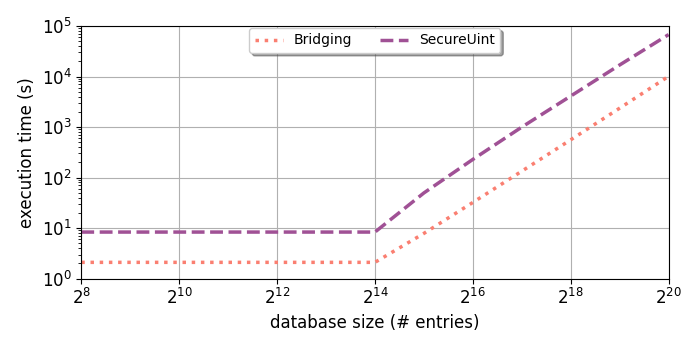
\includegraphics[width=\linewidth]{img/application.png}}
	\caption{Execution time of the setup protocol of a URL denylisting application \cite{urldenylist} implementing the Private Membership Test.}
	\label{fig:application}
\end{figure}

This performance improvement is enabled with just a few tweaks to the sort algorithm.
Consider Listing \ref{list:pmt_sort} presenting this algorithm as an example of modifications required to enable bridged computation.
Function \texttt{sort} reorders the items of a Bloom filter in a sequence known only to the client using encrypted variable \texttt{order}. It creates a list of plaintext indices according to the protocol (lines 10-23), compares homomorphically with the encrypted list of unique permutations sent by the client (variable \texttt{order}), and composes the encrypted Bloom filter \texttt{efilter} with values in this particular order (lines 25-42).

The homomorphic operations start after line 24. There are only a few necessary changes to the algorithm: 1) In lines 1, 26, and 31 we change the return and variable types from \texttt{vector<\secuint<S>{}>} to \texttt{vector<\secmod>}, and 2) in line 35, we cast the \secbool\ type to \secmod, so the subsequent multiplication is done using modular arithmetic.
In bit-level arithmetic it is faster to cast the \texttt{vector<int>} to \secuint\ and multiply by a \secbool, since it results in a \secbool-\secuint\ multiplication instead of a \secuint-\texttt{vector<int>} multiplication. Nevertheless, with bridging it is faster to cast the \secbool\ to \secmod, instead of \texttt{vector<int>}, because \secmod-\texttt{vector<int>} multiplication is faster and less noisy than \secmod-\secmod\ multiplication.
As can be seen in Fig. \ref{fig:application}, Bridging unlocks {\it one order of magnitude} performance improvement, and it only requires minor changes to the source code.

% \subsubsection{Genotype imputation}\label{sss:genotype}
\subsection{Case-study: Genotype imputation}\label{sss:genotype}

Genotype imputation is the process of filling missing information in DNA sequencing with the use of statistical methods. \iffalse Due to the computer-intensive nature of the task, cloud servers are a natural platform for processing the data. Furthermore, privacy requirements of medical information make solutions using homomorphic encryption desirable. \fi P-Impute \cite{GURSOY2021} converts an inefficient statistical model based on correlation of similar individuals %\footnote{The similarity of individuals is determined based on matching single-nucleotide polymorphisms (SNPs) in proximity to the missing SNP.}
into a Private Information Retrieval (PIR) problem, which has efficient solutions in FHE, using the BFV encryption scheme. In this section, we discuss the performance of p-Impute without (\secuint) and with bridging taking into consideration the multiplicative depth for defining more efficient encryption parameters. Batching is used to fit $n$ plaintexts into a ciphertext.

% As this application has much higher memory requirements compared to the previous experiments, we ran the experiments on an Intel Xeon Silver 4214R CPU @ 2.40GHz with 24 cores and 1 TB of memory running on RHEL 7.9. We use the same version of E3 and Microsoft SEAL as in the other experiments with GCC 7.3.1.
We set each run to use 24 threads and report the query time, i.e., the time performing encrypted computation, and the number of ciphertext additions, multiplications, and subtractions in Table \ref{tab:nops}. We use the same plaintext modulus as in the other experiments ($t = 2^{16}+1$), but we vary the polynomial degree ($n \in \{2^{13}, 2^{14}, 2^{15}\}$) in order to evaluate the extra performance improvement provided by bridging for requiring a lower multiplicative depth.
Without bridging, we were only able to run with $n = 2^{15}$, since lower polynomial degrees do not provide enough noise budget to run the application without bootstrapping. %\footnote{Bootstrapping is not supported by Microsoft SEAL library. Accounting for noise growth is commonly tasked to the programmer in FHE applications.}
With bridging, we were able to reduce $n$ to $2^{13}$ without corrupting the result.
As $n$ reduces, the number of batching slots in a ciphertext reduces since it is equal to the polynomial degree. However, the reduction in latency for the homomorphic operation compensates for the reduction in slots. Experimental results show that when $n$ is halved, the latency of the ciphertext multiplication reduces by at least 4 times, and can be amplified depending on the behavior of cache memories. \iffalse This effect can be even greater due to effects related to cache memories.  Therefore, reducing the polynomial degree is always desirable.\fi Consequently, one halving of $n$ increases throughput by at least 2x and reduces latency by 4x.

For the same polynomial degree ($n = 2^{15}$), bridging is around 6.82x faster than bit-level arithmetic. This is due to the reduced number of operations on encrypted data, as one can see in Table \ref{tab:nops}.
Nevertheless, bridging requires less noise budget to operate, which allows us to use smaller polynomial degrees. In the fastest case, bridging has the throughput improved by 62.2x, while the latency reduces by around 249 times.
\vspace{-0.1cm}
\begin{table}[t]
    \centering
    \caption{Number of ciphertext \iffalse additions, multiplications, and subtractions, \fi operations and execution time for p-Impute \cite{GURSOY2021}. \iffalse with and without bridging \replace[and]{using} different polynomial degrees (n).  Without bridging, only $n = 2^{15}$ has enough noise budget for the computation. \fi}
    \vspace{-0.4cm}
    \begin{tabular}{crrrrr}
        Bridging & n &  add  &  mul  &  sub  & time (s) \\ \hline
        \normalfont{no}  & \unboldmath \( 2^{15} \) & \normalfont{53288} & \normalfont{66152} & \normalfont{51256} & \normalfont{5026} \\ \hline
        \normalfont{yes} & \unboldmath \( 2^{15} \) & \normalfont{14248} & \normalfont{ 9072} & \normalfont{ 4536} & \normalfont{ 737} \\ \hline
        \normalfont{no} & \unboldmath \( 2^{14} \) & \normalfont{ NA} & \normalfont{ NA} & \normalfont{ NA} & \normalfont{ NA} \\ 
        \hline
        \normalfont{yes} & \unboldmath \( 2^{14} \) & \normalfont{28496} & \normalfont{18144} & \normalfont{ 9072} & \normalfont{ 196} \\ 
        \hline  
        \normalfont{no} & \unboldmath \( 2^{13} \) & \normalfont{ NA} & \normalfont{ NA} & \normalfont{ NA} & \normalfont{ NA} \\ 
        \hline
        \normalfont{yes} & \unboldmath \( 2^{13} \) & \normalfont{56992} & \normalfont{36288} & \normalfont{18144} & \normalfont{  80} \\ 
             
    \end{tabular}
    \label{tab:nops}
    \vspace{-0.5cm}
\end{table}


\section{Introduction}

With the ever increasing rates of data generation, digital information is becoming extremely valuable over time. As a result, certain types of attacks have emerged, focusing to capitalize on this paradigm shift. To overcome the aforementioned threats, the use of cryptography has been until now the defacto technological security measure to protect against data leakage. Even though accepted standards such as AES have been successful in protecting data-in-transit and data-at-rest, they fail to provide protection towards data-in-use. Hardware solutions \cite{costan2016sgx-explained,trustzone} attempt to provide confidentiality and integrity on sensitive computations, however, a number of attacks \cite{yanga2, hely2012malicious, jin2012exposing, xiao2016hardware, karri2010trustworthy, tsoutsos2013fabrication,adee2008hunt, gross2018ending} including Spectre \cite{Kocher2018spectre}, Meltdown \cite{Lipp2018meltdown}, and Load Value Injection \cite{vanbulck2020lvi}, have raised questions about their effectiveness. Data are eventually decrypted before entering the processor pipeline, and therefore leakage is still possible as recently reported \cite{chen2018sgxpectre}. 

% Consequently, standard encryption algorithms have no effect on data-in-use, as current technology operates exclusively on plaintexts, and therefore requires information to be decrypted before performing any operation on them.

% The latter can be defined as volatile information that is required to undergo certain operations before reaching a state of rest.

% . Intel's software guard extensions (SGX)  and ARM's TrustZone  are two examples of Trusted Execution Environments that allow programmers to protect sensitive data. Even though hardware was believed to be the ultimate root-of-trust, attacks such as Spectre \cite{Kocher2018spectre}, Meltdown \cite{Lipp2018meltdown}, and Load Value Injection \cite{vanbulck2020lvi}, have raised questions about the the validity of this notion.
% Trusted Execution Environments are designed with a fundamental flaw; Data are eventually decrypted before entering the processor pipeline, and therefore leakage is still possible as recently reported \cite{chen2018sgxpectre}


% --------------------
% Along with the AES and other accepted standards, new technologies have also emerged aiming for the improvement of security of data in use. Trusted Execution Environments (TEEs) is one solution that attempts to provide confidentiality and integrity on sensitive computations. As the name implies, TEEs are isolated environments that create the necessary conditions and protection features to securely execute operations. Intel's software guard extensions (SGX) \cite{costan2016sgx-explained} and ARM's TrustZone \cite{trustzone} are two examples of Trusted Execution Environments that allow programmers to protect sensitive data within enclaves, by encrypting all memory traffic in and out of the processor package.

% The appearance of this technology came with a notion that hardware is the ultimate root-of-trust for the software stack. This assumption however, has lately been put at question as attacks such as Spectre \cite{Kocher2018spectre}, Meltdown \cite{Lipp2018meltdown}, and Load Value Injection \cite{vanbulck2020lvi}, keep pilling up. In addition, novel attack trends move closer to the silicon itself. For example, stealthy modifications on hardware designs (i.e., hardware Trojans \cite{yanga2, hely2012malicious, jin2012exposing, xiao2016hardware}), can cause substantial security risks, including privilege escalation, denial of service, information leakage or downgraded performance \cite{karri2010trustworthy, tsoutsos2013fabrication}. Evidently, the lack of hardware-level trust goes beyond academic threat models: There exist folklore reports about a hardware Trojan kill-switch in military air defenses, in the context of electronic warfare \cite{adee2008hunt, gross2018ending}.

% In many contexts, the need for data privacy has been addressed using encryption, which provides implicit access controls to authorized entities with knowledge of a private key. Trusted Execution Environments were once considered a solution to the problem of data security. However, in light of the security threats mentioned above, without end-to-end encryption the privacy risks are merely reduced, but not eliminated. Trusted Execution Environments are designed with a fundamental flaw; Data are eventually decrypted before entering the processor pipeline, and therefore leakage is still possible as recently reported \cite{chen2018sgxpectre}. Consequently, even though encryption can protect data at rest and in transit, protecting \emph{data in use} still remains a challenge.
% %liu2013hardware})

A solution to the problem of protecting data-in-use is Fully Homomorphic Encryption (FHE), as it allows unconstrained computations on ciphertexts. Numerous FHE schemes have been developed, namely BGV~\cite{BGV_ref}, BFV~\cite{fan2012somewhatmisc}, CKKS~\cite{CKKS_ref}, GSW~\cite{GSW_ref}. 
GSW exposes homomorphic Boolean gates and programming computation can be constructed bottom-up.
Such bit-level arithmetic is universal, but requires many Boolean logic operations.
Other schemes, like BGV/BFV, operate directly on integers using modular arithmetic supporting homomorphic addition, subtraction, and multiplication.
At the level of integers however, the operations that can be applied on such ciphertexts are limited to those supported by the encryption scheme.
If an application requires another type of operation like an integer division or comparison, then all computation must be evaluated in bit-level arithmetic, by using arithmetic modulo 2 or algebraic expressions for Boolean gates.

% A solution to the problem of protecting data-in-use is Fully Homomorphic Encryption (FHE), as it allows unconstrained computations on ciphertexts. Since its invention, numerous FHE schemes have been developed, namely BGV~\cite{BGV_ref}, BFV~\cite{fan2012somewhatmisc}, CKKS~\cite{CKKS_ref}, GSW~\cite{GSW_ref}. 
% GSW exposes homomorphic Boolean gates and programming computation can be constructed bottom-up.
% Such bit-level arithmetic is universal, but requires many Boolean logic operations even for addition or multiplication of two numbers.
% Other schemes, like BGV/BFV, operate directly on integers using modular arithmetic supporting homomorphic addition, subtraction, and multiplication.
% At the level of integers, however, the operations that can be applied on such ciphertexts are limited to those supported by the encryption scheme.
% If an application requires another type of operation like an integer division or comparison, then all computation must be evaluated in bit-level arithmetic, by using arithmetic modulo 2 or algebraic expressions for Boolean gates.

% Immediately after its inception in 2009,

In 2009, FHE received criticism on its high computational overheads, which made it challenging at the time to employ in practical applications. Improvements have since been performed on various fronts: 1) Improvement of implementation of FHE libraries. For example, HElib was recently overhauled to achieve almost $75 \times$ performance improvement \cite{cryptoeprint:2018:244}; 2) Hardware acceleration. The developers of nuFHE \cite{nuFHE} report about $100 \times$ acceleration over the software-based implementation of TFHE using GPU hardware. Meanwhile, F1, an ASIC accelerator for the BGV encryption scheme, outperforms software implementations by $5,400 \times$ \cite{f1}; 3) Dedicated programming frameworks. These frameworks allow users to express programming intent directly in a general-purpose programming language, such as Go, Python, C++.
For example, Lattigo~\cite{lattigop} implements  BFV and CKKS schemes in the Go programming language.
PyFHE, PySEAL and Pyfhel~\cite{pyfhel} are frameworks providing Python interface to FHE operations.
\eee\ framework \cite{e3eprint} offers custom C++ data types that can abstract the complexity of FHE library operations. As we observe, native modular arithmetic must be used for logic bit operations; hence program variables must be represented as a sequences of encrypted bits. In such case, \textit{all} programming operations are performed by evaluating Boolean circuits working on encrypted bits - ciphertexts. This transformation makes all computational operations slow, including addition and multiplication.
% Commented out by Homer 
% Nevertheless, in the past decade significant improvements have been made that lead to improvements of several orders of magnitude
% : they are evaluated as Boolean circuits consisting of many gates and each gate operation is composed of modular operations in the direct modular computation. 

\innersection{Our contribution}
In this work, our proposal is to leverage the properties of both (1) bit-level arithmetic (universal, but slower) and (2) modular arithmetic (faster, but not universal) within the same algorithm expressed as a C++ program with custom data types, which allows much better performance of general-purpose programs processing encrypted data. 
Towards that end, we extend the E3 programming framework \cite{e3eprint} and implement \emph{Bridging}, which enables the mixing of different arithmetic abstractions in the same C++ program that processes FHE data.
The benefit of using our method is a significant application performance improvement, as we demonstrate with our experiments.

% \innersection{Paper roadmap}
% Section \ref{s:preliminaries} introduces key concepts of homomorphic encryption, data-oblivious programming, and FHE schemes. In Section \ref{s:bridging}, we present our proposal and demonstrate how bridging can significantly improve the performance of FHE applications. Experimental results are evaluated in Section \ref{s:results} with synthetic benchmarks and real-world applications. Related work is available in Section \ref{s:related_work}. Finally, in Section \ref{s:conclusions}, we conclude our paper with the main insights.
% \subsubsection{Genotype imputation}\label{sss:genotype}
\subsection{Case-study: Genotype imputation}\label{sss:genotype}

Genotype imputation is the process of filling missing information in DNA sequencing with the use of statistical methods. \iffalse Due to the computer-intensive nature of the task, cloud servers are a natural platform for processing the data. Furthermore, privacy requirements of medical information make solutions using homomorphic encryption desirable. \fi P-Impute \cite{GURSOY2021} converts an inefficient statistical model based on correlation of similar individuals %\footnote{The similarity of individuals is determined based on matching single-nucleotide polymorphisms (SNPs) in proximity to the missing SNP.}
into a Private Information Retrieval (PIR) problem, which has efficient solutions in FHE, using the BFV encryption scheme. In this section, we discuss the performance of p-Impute without (\secuint) and with bridging taking into consideration the multiplicative depth for defining more efficient encryption parameters. Batching is used to fit $n$ plaintexts into a ciphertext.

% As this application has much higher memory requirements compared to the previous experiments, we ran the experiments on an Intel Xeon Silver 4214R CPU @ 2.40GHz with 24 cores and 1 TB of memory running on RHEL 7.9. We use the same version of E3 and Microsoft SEAL as in the other experiments with GCC 7.3.1.
We set each run to use 24 threads and report the query time, i.e., the time performing encrypted computation, and the number of ciphertext additions, multiplications, and subtractions in Table \ref{tab:nops}. We use the same plaintext modulus as in the other experiments ($t = 2^{16}+1$), but we vary the polynomial degree ($n \in \{2^{13}, 2^{14}, 2^{15}\}$) in order to evaluate the extra performance improvement provided by bridging for requiring a lower multiplicative depth.
Without bridging, we were only able to run with $n = 2^{15}$, since lower polynomial degrees do not provide enough noise budget to run the application without bootstrapping. %\footnote{Bootstrapping is not supported by Microsoft SEAL library. Accounting for noise growth is commonly tasked to the programmer in FHE applications.}
With bridging, we were able to reduce $n$ to $2^{13}$ without corrupting the result.
As $n$ reduces, the number of batching slots in a ciphertext reduces since it is equal to the polynomial degree. However, the reduction in latency for the homomorphic operation compensates for the reduction in slots. Experimental results show that when $n$ is halved, the latency of the ciphertext multiplication reduces by at least 4 times, and can be amplified depending on the behavior of cache memories. \iffalse This effect can be even greater due to effects related to cache memories.  Therefore, reducing the polynomial degree is always desirable.\fi Consequently, one halving of $n$ increases throughput by at least 2x and reduces latency by 4x.

For the same polynomial degree ($n = 2^{15}$), bridging is around 6.82x faster than bit-level arithmetic. This is due to the reduced number of operations on encrypted data, as one can see in Table \ref{tab:nops}.
Nevertheless, bridging requires less noise budget to operate, which allows us to use smaller polynomial degrees. In the fastest case, bridging has the throughput improved by 62.2x, while the latency reduces by around 249 times.
\vspace{-0.1cm}
\begin{table}[t]
    \centering
    \caption{Number of ciphertext \iffalse additions, multiplications, and subtractions, \fi operations and execution time for p-Impute \cite{GURSOY2021}. \iffalse with and without bridging \replace[and]{using} different polynomial degrees (n).  Without bridging, only $n = 2^{15}$ has enough noise budget for the computation. \fi}
    \vspace{-0.4cm}
    \begin{tabular}{crrrrr}
        Bridging & n &  add  &  mul  &  sub  & time (s) \\ \hline
        \normalfont{no}  & \unboldmath \( 2^{15} \) & \normalfont{53288} & \normalfont{66152} & \normalfont{51256} & \normalfont{5026} \\ \hline
        \normalfont{yes} & \unboldmath \( 2^{15} \) & \normalfont{14248} & \normalfont{ 9072} & \normalfont{ 4536} & \normalfont{ 737} \\ \hline
        \normalfont{no} & \unboldmath \( 2^{14} \) & \normalfont{ NA} & \normalfont{ NA} & \normalfont{ NA} & \normalfont{ NA} \\ 
        \hline
        \normalfont{yes} & \unboldmath \( 2^{14} \) & \normalfont{28496} & \normalfont{18144} & \normalfont{ 9072} & \normalfont{ 196} \\ 
        \hline  
        \normalfont{no} & \unboldmath \( 2^{13} \) & \normalfont{ NA} & \normalfont{ NA} & \normalfont{ NA} & \normalfont{ NA} \\ 
        \hline
        \normalfont{yes} & \unboldmath \( 2^{13} \) & \normalfont{56992} & \normalfont{36288} & \normalfont{18144} & \normalfont{  80} \\ 
             
    \end{tabular}
    \label{tab:nops}
    \vspace{-0.5cm}
\end{table}


\subsubsection{\secint\ to \secmod{}}\label{sss:secint2secmod}

So far, we have discussed unsigned numbers. However, bit-level arithmetic also supports signed numbers following the two's complement arithmetic.
On the other hand, modular arithmetic only supports numbers in $\mathbb{Z}_t$, where $t$ is the plaintext modulus.
Nevertheless, it is possible to emulate negative numbers in modular arithmetic in the programmer's domain as in Cryptoleq \cite{cryptoleq}, where lower values are considered positive and large values are interpreted as negative numbers.
In this case, the conversion from a signed bit-level arithmetic type \secint\ to \secmod\ is defined as:
\begin{equation}
  X=\begin{cases}
    t - 2^s + \sum_{i=0}^{s-1}{(2^i \cdot x_i)}, & \text{if $x<0$}.\\
    \sum_{i=0}^{s-1}{(2^i \cdot x_i)}, & \text{otherwise}.
  \end{cases}
\end{equation}
where $s$ is the number of bits and $x_i$ is the bit of $x$ at position $i$. The condition $x < 0$ is determined by the most significant bit of $x$; thus, we can use it as a multiplexer between the two cases.
Listing \ref{list:secint2secmod} presents the algorithm for converting a \secint\ into a \secmod. First, the \secint\ is interpreted as a \secuint\ (line 4). In line 5, this value is converted into a \secmod\ using the algorithm of Listing \ref{list:secuint2secmod}.
Then in line 7, we perform the subtraction of plaintexts $t$ and \texttt{max} (i.e. $2^s$), and then do a ciphertext addition with the \secmod\ variable \texttt{pos}. At this point, we have generated two \secmod\ variables: \texttt{pos}, representing the value in case it is positive, and \texttt{neg} containing the value in case it is a negative number. This totals $2s - 1$ ciphertext additions with a additive depth of $s$.
Finally, we select between \texttt{neg} and \texttt{pos} using the most significant bit of the \secint\ input (lines 8-9). If the bit is one, it means it is a negative number; thus, we select \texttt{neg}; otherwise, we select \texttt{pos}.
For selection we need ciphertext multiplications.
The entire conversion from \secint\ to \secmod\ requires two ciphertext multiplications and $2s + 1$ ciphertext additions with a multiplicative depth equal to one.
By comparing Listings \ref{list:secuint2secmod} and \ref{list:secint2secmod}, we can see that converting signed numbers to \secmod\ is less efficient than converting unsigned numbers to \secmod. Furthermore, $t$ must be large enough ($t \geq 2^s$) to accommodate the converted value.

% \innersection{Why not signed and unsigned \secmod{}} \secmod{} types can only participate in addition, subtraction, and multiplication operations. The values of this type are elements of the corresponding mathematical ring. The programmer can choose to interpret a subset of the number space as negative, but there would be no difference in these computations. For this reason, there is no differentiation between the signed and unsigned versions for \secmod{} type.
\subsection{Conversion}\label{ss:conversion}

Fig. \ref{fig:tosecmod} presents the conversion latency time from \secuint\ and \secint\ to \secmod\ for different bit sizes following the algorithms of Listings \ref{list:secuint2secmod} and \ref{list:secint2secmod}. The number of multiplications for \secuint\ and \secint\ stays constant at 0 and 2, while the multiplicative depth is 0 and 1, respectively, for all bit sizes. 
\iffalse As discussed in Section \ref{ss:bridging}, converting from \secint\ is slower than converting from \secuint\ because a \secint\ to \secmod\ conversion uses two ciphertext multiplications to account for the sign \fi . As expected, conversion from both \secuint\ and \secint\ becomes slower for larger bit sizes due to the larger number of additions required. The slowdown is the same for both types. It is less noticeable for \secint\ due the log-scale graph and the fact that the multiplications dominate the \secint\ latency time.

\begin{figure}[t]
	\centering
    \frame{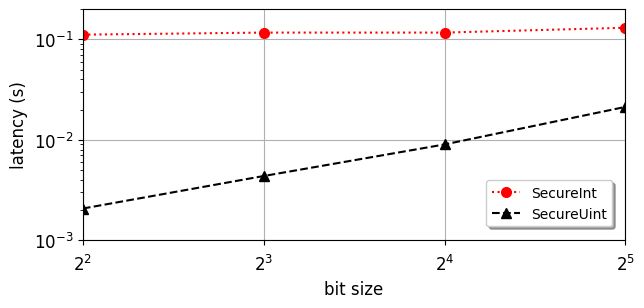
\includegraphics[width=\linewidth]{img/toSecureMod.png}}
	\caption{Conversion latency time from \secuint\ and \secint\ to \secmod\ for different bit sizes. Throughput is up to $n=2^{15}$ times faster since a ciphertext fits $n$ plaintexts.}
	\label{fig:tosecmod}
	\vspace{-0.6cm} 
\end{figure}

We also evaluate the conversion latency time from \secmod\ to \secuint/\secint\ using the algorithms presented in Listings \ref{list:secmod2secuint} and \ref{list:secmod2secint} with different plaintext moduli and bit sizes ($s = \{4, 8, 16, 32\}$). Fig.~\ref{fig:fromsecmod} summarizes the findings.
The results are what we expect from analysing the algorithms in Listings \ref{list:secmod2secuint} and \ref{list:secmod2secint}: When converting from \secmod\ to \secuint, the latency increases linearly to the bit size due to the operation on line 11 of Listing \ref{list:secmod2secuint}. Nevertheless, the dominant factor is the plaintext modulus $t$. A minor logarithmic effect comes from the exponentiation function (line 10) where the number of multiplications increases, while a major linear effect comes from the larger number of iterations in the \texttt{for} loop (line 7).
The conversion from \secmod\ to \secint\ (Listing \ref{list:secmod2secint}) takes roughly twice the time since it consists of two calls to the \secmod\ to \secuint\ conversion (lines 4 and 8) plus two multiplications (line 11).

\begin{figure}[t]
	\centering
    \frame{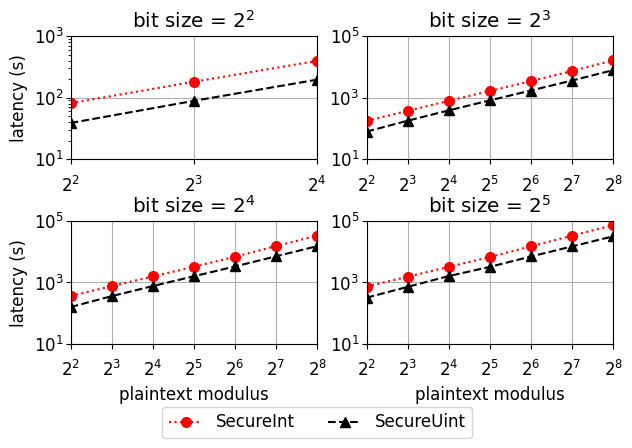
\includegraphics[width=\linewidth]{img/fromSecureMod.png}}
	\caption{Conversion latency time from \secmod\ to \secuint\ and \secint\ for different plaintext moduli and bit sizes.}
	\label{fig:fromsecmod}
	\vspace{-0.5cm}
\end{figure}



% \innersection{Insights}
% The results show that the conversion from bit-level to modular arithmetic is fast and can be used in practice. Meanwhile, converting from modular to bit-level arithmetic has borderline practical times only for very small plaintext moduli. With an small increase in the plaintext modulus, it quickly becomes prohibitive.

\subsubsection{\secmod\ to \secuint{}}\label{sss:secmod2secuint}
\vspace{-0.2cm}
Conversion from \secmod\ to \secuint\ is theoretically possible using the expression:
\vspace{-0.2cm}
\begin{equation}\label{eq:secmod2secuint}
    \vspace{-0.1cm}
    X = \sum_{i=1}^{t-1}(i \cdot \secbool(1 - (x-i)^{t-1}))
\end{equation}
where $x$ is the \secmod\ variable to be converted, $t$ is the plaintext modulus and is prime, $i$ is a \secuint\ counter, and $X$ is the resulting \secuint. Due to the properties of modular arithmetic and the parameters used in homomorphic encryption, the exponentiation to $t-1$ results in zero in case the base is zero, and one otherwise. When $i = x$, the expression in the summation results in $i$, while in all other cases it will result in zero, since $1 - (x-i)^{t-1} = 0 \ \forall \ i \ne x$.
% Breaking down Eq. \ref{eq:secmod2secuint}:
% \begin{enumerate}
%     \item The \secuint\ $i$ is automatically cast to \secmod\ in $x-i$ before the exponentiation, resulting in a subtraction between two \secmod{}s.
%     \item The exponentiation of the \secmod\ $x-i$ to the integer $t-1$ results in a \secmod\ variable containing either the encryption of zero or one.
%     \item The result of the exponentiation is negated by subtracting it from one. At this point, we have the encryption of one in case $x = i$ and zero otherwise stored in a \secmod\ variable. In order to avoid automatically casting $i$ to \secmod\ in the multiplication, we must first reinterpret the partial result as \secbool.
%     \item We multiply the \secuint\ $i$ by the \secbool\ value resulting in a \secuint\ equal to $i$ or zero. We remark that a \secbool-\secuint\ multiplication is evaluated as a multiplexer operation.
%     \item We repeat this process for all $i \in [1,t)$, adding the resulting values. The final result is a \secuint\ equal to $x$ since there is only one $i$ that is equal to $x$.
% \end{enumerate}

An implementation of the fast exponentiation algorithm is presented in Listing \ref{list:pow}. The number of multiplications is given by $\floor{\log_2{e}} + \omega(e) - 1$ and the multiplicative depth is $\ceil{\log_2{e}}$, where $e$ is the exponent and $\omega(\cdot)$ is a function that calculates the Hamming weight. The conversion from \secmod\ to \secuint\ can exploit this property of the exponentiation to $t-1$ resulting in zero or one to create an equality function, where the equality function is given by $1 - (x-i)^{t-1}$. With this information, we can build a linear search to find the \secuint\ $i$ that is equal to the \secmod\ $x$ using the result of the equality as a selector. Listing \ref{list:secmod2secuint} presents the algorithm that performs this conversion.
The number of multiplications is given by $t \cdot (s + \floor{\log_2{(t-1)}} + \omega(t-1) - 1)$, while the multiplicative depth is equal to $\ceil{\log_2{(t-1)}} + 1$.
One can notice that this algorithm is only practical for small plaintext moduli $t$. Once $t$ becomes large, the linear search makes it impractical. Since \secmod\ requires a large $t$ for it to be useful, this conversion should not be used in practice and should be avoided, as later presented and discussed in Section~\ref{ss:conversion}.

\begin{figure}[t]
%\scriptsize
\begin{minipage}{\linewidth}
\begin{lstlisting}[language=C++, caption={
Homomorphic exponentiation function.}, style=mystyleb, label=list:pow,
%framexrightmargin=-37pt,
% xleftmargin=0.4cm,
% xrightmargin=-0.12\linewidth,
% linewidth=0.88\linewidth
]
SecureMod pow(SecureMod b, int e)
{
    if (e == 0) return SecureMod(1);
    if (e == 1) return b;
    auto r = pow(b * b, e >> 1);
    if (e & 1) r *= b;
    return r;
}
\end{lstlisting}
\end{minipage}
% \vspace{\lstbspace}
\vspace{-0.5cm} 
\end{figure}

\begin{figure}[!t]
%\scriptsize
\begin{minipage}{\linewidth}
\begin{lstlisting}[language=C++, caption={
Casting from \secmod\ to \secuint.}, style=mystyleb, label=list:secmod2secuint,
%framexrightmargin=-37pt,
% xleftmargin=0.4cm,
% xrightmargin=-0.12\linewidth,
% linewidth=0.88\linewidth
]
template <int Size>
SecureUint to_SecureUint<Size>(SecureMod x)
{
SecureMod one(1);
    auto & t = SecureMod::t;
    vector<SecureUint<Size>> v;
    for (int i = 1; i < t; i++)
    {
        auto si = SecureUint<Size>(i);
        auto eq = one - pow(x-i, t-1);
        v.push_back(si * SecureBool(eq));
    }
    return sum(v);
}
\end{lstlisting}
\end{minipage}
% \vspace{\lstbspace}
\vspace{-0.5cm} 
\end{figure}

\section{Discussion}\label{s:related_work}

\noindent {\bf Polynomial degree:}
We compare bridging with other accelerations of homomorphic computation at the programming level.
% \vspace{-0.5cm}
As we show in Section \ref{sss:genotype}, the polynomial degree affects the performance and noise budget. A smaller polynomial degree makes operations a few times faster. At the same time, it reduces the noise budget, allowing fewer computations before data corruption or bootstrapping. It also reduces the number of plaintexts that can be packed in a ciphertext when batching. Nevertheless, the performance improvement from a smaller polynomial degree outweighs the fewer batching slots in the ciphertexts.
% The best option is to use the smallest polynomial degree that does not corrupt the ciphertext. 

\noindent {\bf Batching} enables SIMD usage of ciphertexts \cite{batching}. It can provide several orders of magnitude performance improvement for SIMD-compatible applications, however not all FHE schemes support it \cite{chillotti2016faster,ducas2015fhew}. Due to its significant computational benefits, batching should always be used where possible. \iffalse if the target application is compatible with it. \fi

% Unfortunately, not all FHE schemes support batching (e.g., TFHE \cite{chillotti2016faster} and FHEW \cite{ducas2015fhew}). The ones that do, such as BGV \cite{BGV_ref} or BFV \cite{fan2012somewhatmisc}, support it only for some specific encryption parameters, which may not be the most noise efficient parameters for the target application.
% In any case, due to its significant performance benefits, batching should always be used if the target application is compatible with it.

\noindent {\bf Bridging} makes possible to use the comprehensive bit-level arithmetic and the fast modular arithmetic in the same program. It increases the expressivity of programs previously limited to modular arithmetic, and improves performance of complex programs implemented using bit-level arithmetic. At the same time, it reduces noise, since the depth of the datapath is shorter due to fewer homomorphic operations being executed, which may enable using a smaller polynomial degree, further improving performance.
Therefore, the performance improvement provided by bridging comes from two factors: 1) Reduced number of homomorphic operations since Boolean circuits performing additions and multiplications in bit-level arithmetic are replaced by a single operation (native addition or multiplication), and 2) reduced multiplicative depth, since when Boolean circuits are replaced by a single instruction, the multiplicative depth reduces. This reduces the noise budget required by the application, enabling the use of a smaller polynomial degree, further improving performance.
In addition, bridging is independent of encryption parameters, apart from the plaintext modulus which should not be too small. This makes bridging perfectly compatible with batching and any polynomial degree.

% \noindent {\bf Class of programs benefiting from bridging}:
% FHE itself is already introducing restrictions on the class of programs that can be practically used with FHE-encrypted data. Within the subset of applications that have demonstrated such potential, the algorithms that benefit the most from bridging should have all non-native operations at the beginning of computation with the remaining computation using only native operations. This applies well to the algorithms involving data selection followed by computation on selected data. Therefore, examples of such classes of programs are 1) membership tests (case study 1 - URL denylist), 2) information retrieval, 3) set intersections, and 4) keyword search (case study 2 - genotype imputation). On the other hand, algorithms having non-native operations throughout the computation or near its output would not benefit from bridging. This is the case for sorting algorithms, which are mostly comparisons, and some block ciphers algorithms that are heavy on bit-wise operations.
\subsection{Overview and setup}\label{ss:setup}

We evaluate bridging using three sets of experiments:
\begin{enumerate}
    \item Conversion from \secuint\ and \secint\ to \secmod, and vice-versa, using different bit sizes.
    \item Performance comparison of bridging and bit-level arithmetic using synthetic benchmarks.
    \item Case study analysis using one real-world FHE application.
\end{enumerate}

% The results presented in Sections \ref{ss:conversion} and \ref{ss:benchmarks} were collected using a single thread of an Intel i7-4790 CPU @ 3.60GHz with 16 GB of RAM, 64 GB of swap area, running Ubuntu 18.04.5, with GCC 9.4.0.\footnote{Due to memory requirements, the setup for the genotype imputation case study differs and is defined locally in the section.} We use the E3 framework (commit \#9fb718f) with SEAL 3.3.2 as underlying FHE library, and BFV as the encryption scheme. We set the encryption parameters as: polynomial degree $n = 2^{15}$, as it provides the largest noise budget for encrypted computation, and plaintext modulus $t = 2^{16}+1$, as this is the smallest $t$ that enables batching for the chosen $n$. While a smaller $t$ would provide less noisy homomorphic operations, virtually all practical FHE applications rely on efficient utilization of batching. Nevertheless, although $t=2$ does not enable batching on BFV, we also test it on the benchmarks (Section \ref{ss:benchmarks}) since some homomorphic gates are simpler in modulo 2. The remaining parameters are automatically defined by SEAL given the required security level of 128 bits.

% As this application has much higher memory requirements compared to the previous experiments, we ran the experiments on an Intel Xeon Silver 4214R CPU @ 2.40GHz with 24 cores and 1 TB of memory running on RHEL 7.9. We use the same version of E3 and Microsoft SEAL as in the other experiments with GCC 7.3.1.
The results presented in Section \ref{s:results} were collected using a single thread (Sections \ref{ss:conversion} and \ref{ss:benchmarks}) and 24 threads (Section \ref{sss:genotype}) of an Intel Xeon Silver 4214R CPU @ 2.40GHz with 24 cores and 1 TB of memory running on RHEL 7.9, with GCC 7.3.1. We use the E3 framework (commit \#9fb718f) with SEAL 3.3.2 \cite{seal} as underlying FHE library, and BFV as the encryption scheme. We set the encryption parameters as: polynomial degree $n = 2^{15}$, as it provides the largest noise budget for encrypted computation, and plaintext modulus $t = 2^{16}+1$, as this is the smallest $t$ that enables batching for the chosen $n$. While a smaller $t$ would provide less noisy homomorphic operations, virtually all practical FHE applications rely on efficient utilization of batching. Nevertheless, although $t=2$ does not enable batching on BFV, we also test it on the benchmarks (Section \ref{ss:benchmarks}) since some homomorphic gates are simpler in modulo 2. The remaining parameters are automatically defined by SEAL given the required security level of 128 bits.
\subsubsection{URL denylisting}
\label{ss:url}
\begin{figure}[h!]
% \vspace{-0.2 cm}
\begin{minipage}{\linewidth}
\begin{lstlisting}[language=C++, caption={
Relevant function of the setup protocol of the URL denylisting application with bridging.
},
style=mystyle, 
label=list:pmt_sort,
xleftmargin=0.45cm,
% xrightmargin=-0.12\linewidth,
% linewidth=0.88\linewidth
]
template <int S> vector<SecureMod>
sort (int logt, vector<int> filter,
  const vector<SecureUint<S>> & order)
{
  using SecUint = SecureUint<S>;
  auto s = order.size();
  auto n = SecureMod::slots();
  auto nsp = n*s*logt;
  filter.resize(nsp, 0);
  vector<vector<unsigned>> f;
  for (int i=0; i<s; i++)
  {
    vector<unsigned> poly;
    for (int j=0; j<n; j++)
    {
      unsigned plain = 0;
      for (int k=0; k<logt; k++)
        plain = (plain<<1) +
          bool( filter[i+(j*logt+k)*s] );
      poly.push_back(plain);
    }
    f.push_back(poly);
  }
  
  $//$vector<SecUint> efilter;
  vector<SecureMod> efilter;
  for ( int i=0; i<s; i++ )
  {
    const auto & c = order[i];
    $//$vector<SecUint> partial_res;
    vector<SecureMod> partial_res;
    for (int j=0; j<s; j++)
    {
      $//$auto tmp = (c==j) * SecUint(f[j]);
      auto tmp = SecureMod(c==j) * f[j];
      partial_res.push_back(tmp);
    }
    $//$ low depth array summation  
    auto r = sum(partial_res);
    efilter.push_back(r);
  }
  return efilter;
}
\end{lstlisting}
\end{minipage}
\vspace{-0.6 cm}
% \vspace{-0.1 cm}
\end{figure}

We evaluate the performance improvements provided by bridging using a URL denylisting application as a case study \cite{urldenylist}.
The application implements a Private Membership Test (PMT) protocol, a common cryptographic building block for privacy-preserving applications.
Its main operation is checking if an element is part of a database without revealing information about the element.
In this scenario, the server hosting the database is semi-trusted (honest-but-curious).

URL denylisting is the process where a URL is being checked against a known database of malicious URLs; if there is a match, the access to the website is blocked. URL denylisting can be used in conjunction with URL rewriting to protect against e-mail phishing attacks. In other words, when an email comes to the company server, its URLs are being replaced by a redirection to the service provider site, which checks whether the link is malicious or not. If it is benign, the user is automatically forwarded to the webpage. While this (supposedly) protects against phishing attacks, it introduces a huge privacy problem, since the company hosting the service can clearly see which links the users are visiting, and can potentially sell the data to other parties. 

The PMT protocol we evaluate here is composed of two main phases: setup and query. In the setup phase, the database is converted into a format that enables fast queries. The query phase is simply checking if a particular element is part of the database.
While queries are fast, the setup is expensive since it uses comparison operations. As mentioned in the previous sections, comparisons require bit-level arithmetic, leading to execution times of more than a day for databases with millions of entries. Implementing a faster setup protocol is therefore critical to the practicality of the application. 

The setup protocol is composed of three main stages: 1) The server database containing the list of malicious URLs is converted into a Bloom filter \cite{bloomfilter}. The server then informs the size of this Bloom filter $m$ to the client. 2) In the next step, the client creates a list with random permutations of \mbox{$\ceil{ {m}/({n \cdot \floor{\log_{2}{t}}} ) }$} unique integers, where $m$ is the size of the Bloom filter, $n$ is the polynomial degree, and $t$ is the plaintext modulus. The client encrypts the list with its public key and sends to the server. 3) Finally, the server runs a particular homomorphic algorithm that sorts the Bloom filter into a way only known to the client. This produces an encrypted Bloom filter in this particular order.

Out of the three stages in the setup, only the third one operates homomorphically on encrypted data. Therefore, we implemented the third stage of the setup protocol using bridging and compared its performance against the bit-level arithmetic implementation.
As shown in Fig. \ref{fig:application}, bridging provides approximately one order of magnitude of performance improvement for this application, reducing the setup time for databases with one million entries to less than three hours, instead of more than a day when bit-level arithmetic is exclusively used.

\begin{figure}[t]
	\centering
    \frame{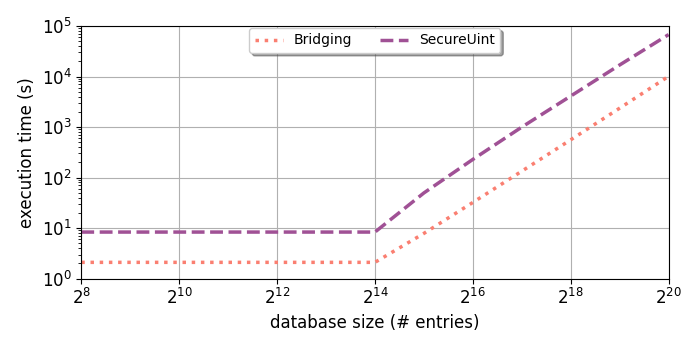
\includegraphics[width=\linewidth]{img/application.png}}
	\caption{Execution time of the setup protocol of a URL denylisting application \cite{urldenylist} implementing the Private Membership Test.}
	\label{fig:application}
\end{figure}

This performance improvement is enabled with just a few tweaks to the sort algorithm.
Consider Listing \ref{list:pmt_sort} presenting this algorithm as an example of modifications required to enable bridged computation.
Function \texttt{sort} reorders the items of a Bloom filter in a sequence known only to the client using encrypted variable \texttt{order}. It creates a list of plaintext indices according to the protocol (lines 10-23), compares homomorphically with the encrypted list of unique permutations sent by the client (variable \texttt{order}), and composes the encrypted Bloom filter \texttt{efilter} with values in this particular order (lines 25-42).

The homomorphic operations start after line 24. There are only a few necessary changes to the algorithm: 1) In lines 1, 26, and 31 we change the return and variable types from \texttt{vector<\secuint<S>{}>} to \texttt{vector<\secmod>}, and 2) in line 35, we cast the \secbool\ type to \secmod, so the subsequent multiplication is done using modular arithmetic.
In bit-level arithmetic it is faster to cast the \texttt{vector<int>} to \secuint\ and multiply by a \secbool, since it results in a \secbool-\secuint\ multiplication instead of a \secuint-\texttt{vector<int>} multiplication. Nevertheless, with bridging it is faster to cast the \secbool\ to \secmod, instead of \texttt{vector<int>}, because \secmod-\texttt{vector<int>} multiplication is faster and less noisy than \secmod-\secmod\ multiplication.
As can be seen in Fig. \ref{fig:application}, Bridging unlocks {\it one order of magnitude} performance improvement, and it only requires minor changes to the source code.

\section{Conclusions}\label{s:conclusions}

In this work, we presented a new methodology combining universal bit-level arithmetic and faster modular arithmetic computation, dubbed \emph{bridging}, to accelerate applications using fully homomorphic encryption. Experiments demonstrate significant performance improvements when using both bridging and batching modes. Bridging by itself can offer several orders of magnitude performance improvement, depending on the type of application. \iffalse In the worst case, bridging offers no performance improvement, but also no performance degradation. Applications with complex operations requiring bit-level arithmetic at the beginning of execution followed by long operations on modular arithmetic are the ones that benefit the most from bridging. \fi In the benchmark evaluation, bridging improved performance by more than 2 orders, and 6 orders of magnitude when combined with batching. 
Furthermore, the case-study private genotype imputation became two orders of magnitude faster due to reduced number of homomorphic operations and multiplicative depth, allowing us to use more efficient encryption parameters.

%%
%% This is file `sample-sigconf.tex',
%% generated with the docstrip utility.
%%
%% The original source files were:
%%
%% samples.dtx  (with options: `sigconf')
%% 
%% IMPORTANT NOTICE:
%% 
%% For the copyright see the source file.
%% 
%% Any modified versions of this file must be renamed
%% with new filenames distinct from sample-sigconf.tex.
%% 
%% For distribution of the original source see the terms
%% for copying and modification in the file samples.dtx.
%% 
%% This generated file may be distributed as long as the
%% original source files, as listed above, are part of the
%% same distribution. (The sources need not necessarily be
%% in the same archive or directory.)
%%
%% Commands for TeXCount
%TC:macro \cite [option:text,text]
%TC:macro \citep [option:text,text]
%TC:macro \citet [option:text,text]
%TC:envir table 0 1
%TC:envir table* 0 1
%TC:envir tabular [ignore] word
%TC:envir displaymath 0 word
%TC:envir math 0 word
%TC:envir comment 0 0
%%
%%
%% The first command in your LaTeX source must be the \documentclass command.
\documentclass[sigconf]{acmart}
%% NOTE that a single column version is required for 
%% submission and peer review. This can be done by changing
%% the \doucmentclass[...]{acmart} in this template to 
%% \documentclass[manuscript,screen]{acmart}
%% 
%% To ensure 100% compatibility, please check the white list of
%% approved LaTeX packages to be used with the Master Article Template at
%% https://www.acm.org/publications/taps/whitelist-of-latex-packages 
%% before creating your document. The white list page provides 
%% information on how to submit additional LaTeX packages for 
%% review and adoption.
%% Fonts used in the template cannot be substituted; margin 
%% adjustments are not allowed.

% \usepackage[utf8]{inputenc}%(only for the pdftex engine)
% %\RequirePackage[no-math]{fontspec}%(only for the luatex or the xetex engine)
% \usepackage[big]{dgruyter_NEW}

\usepackage{balance}
% \usepackage{amsmath,amssymb,amsfonts}
\usepackage{amsmath,amsfonts}
\usepackage{algorithmic}
\usepackage{color}
\usepackage{enumitem}
\usepackage{fancyhdr}
\usepackage{graphicx}
\usepackage[utf8]{inputenc}
\usepackage{listings}
\usepackage{makecell}
\usepackage{mathtools}
% \usepackage{mathptmx} % This is Times font
\usepackage{microtype}
\usepackage{multirow}
\usepackage{pifont}
\usepackage{tablefootnote}
\usepackage{textcomp}
\usepackage[flushleft]{threeparttable}
\usepackage[normalem]{ulem}
\usepackage{xcolor}
\sloppy

\useunder{\uline}{\ul}{}

\newcommand{\Plots}{\texttt{Plots.jl}~}
\newcommand{\RecipesBase}{\texttt{RecipesBase.jl}~}

%%
%% \BibTeX command to typeset BibTeX logo in the docs
\AtBeginDocument{%
  \providecommand\BibTeX{{%
    \normalfont B\kern-0.5em{\scshape i\kern-0.25em b}\kern-0.8em\TeX}}}

%% Rights management information.  This information is sent to you
%% when you complete the rights form.  These commands have SAMPLE
%% values in them; it is your responsibility as an author to replace
%% the commands and values with those provided to you when you
%% complete the rights form.
\copyrightyear{2022}
\acmYear{2022}
\setcopyright{acmlicensed}\acmConference[ICCAD '22]{IEEE/ACM International Conference on Computer-Aided Design}{October 30-November 3, 2022}{San Diego, CA, USA}
\acmBooktitle{IEEE/ACM International Conference on Computer-Aided Design (ICCAD '22), October 30-November 3, 2022, San Diego, CA, USA}
\acmPrice{15.00}
\acmDOI{10.1145/3508352.3549415}
\acmISBN{978-1-4503-9217-4/22/10}

% \setcopyright{acmcopyright}
% \copyrightyear{2022}
% \acmYear{2022}
% \acmDOI{XXXXXXX.XXXXXXX}

% %% These commands are for a PROCEEDINGS abstract or paper.
% \acmConference[ICCAD '22]{IEEE/ACM 2022 International Conference on Computer-Aided Design}{October 30--November 03,
%   2022}{San Diego, CA, USA}
% %
% %  Uncomment \acmBooktitle if th title of the proceedings is different
% %  from ``Proceedings of ...''!
% %
% %\acmBooktitle{Woodstock '18: ACM Symposium on Neural Gaze Detection,
% %  June 03--05, 2018, Woodstock, NY} 
% \acmPrice{15.00}
% \acmISBN{978-1-4503-XXXX-X/18/06}


%%
%% Submission ID.
%% Use this when submitting an article to a sponsored event. You'll
%% receive a unique submission ID from the organizers
%% of the event, and this ID should be used as the parameter to this command.
%%\acmSubmissionID{123-A56-BU3}

%%
%% For managing citations, it is recommended to use bibliography
%% files in BibTeX format.
%%
%% You can then either use BibTeX with the ACM-Reference-Format style,
%% or BibLaTeX with the acmnumeric or acmauthoryear sytles, that include
%% support for advanced citation of software artefact from the
%% biblatex-software package, also separately available on CTAN.
%%
%% Look at the sample-*-biblatex.tex files for templates showcasing
%% the biblatex styles.
%%

%%
%% The majority of ACM publications use numbered citations and
%% references.  The command \citestyle{authoryear} switches to the
%% "author year" style.
%%
%% If you are preparing content for an event
%% sponsored by ACM SIGGRAPH, you must use the "author year" style of
%% citations and references.
%% Uncommenting
%% the next command will enable that style.
%%\citestyle{acmauthoryear}

%%
%% end of the preamble, start of the body of the document source.
\begin{document}

%%
%% The "title" command has an optional parameter,
%% allowing the author to define a "short title" to be used in page headers.
\title[Accelerating Fully Homomorphic Encryption by Bridging Modular and Bit-Level Arithmetic]
{Accelerating Fully Homomorphic Encryption\\by Bridging Modular and Bit-Level Arithmetic}

%%
%% The "author" command and its associated commands are used to define
%% the authors and their affiliations.
%% Of note is the shared affiliation of the first two authors, and the
%% "authornote" and "authornotemark" commands
%% used to denote shared contribution to the research.

\author{Eduardo Chielle, Oleg Mazonka, Homer Gamil, and Michail Maniatakos}
\affiliation{
    \institution{Center for Cyber Security, New York University Abu Dhabi, Abu Dhabi, UAE}
    \country{}
}
\email{{eduardo.chielle, om22, homer.g, michail.maniatakos}@nyu.edu}

% \author{Eduardo Chielle}
% % \email{trovato@corporation.com}
% \orcid{0000-0002-1938-912X}
% \affiliation{%
%   \institution{New York University Abu Dhabi}
% %   \streetaddress{P.O. Box 1212}
% %   \city{Abu Dhabi}
% %   \state{Ohio}
% %   \country{UAE}
% %   \postcode{43017-6221}
% }

% \author{Oleg Mazonka}
% \affiliation{%
%   \institution{New York University Abu Dhabi}
% %   \streetaddress{P.O. Box 1212}
% %   \city{Abu Dhabi}
% %   \state{Ohio}
% %   \country{UAE}
% %   \postcode{43017-6221}
% }

% \author{Homer Gamil}
% \affiliation{%
%   \institution{New York University}
% %   \streetaddress{P.O. Box 1212}
% %   \city{New York}
% %   \state{NY}
% %   \country{USA}
% %   \postcode{43017-6221}
% }

% \author{Michail Maniatakos}
% \affiliation{%
%   \institution{New York University Abu Dhabi}
% %   \city{Abu Dhabi}
% %   \country{UAE}
% }

% \author{}

%%
%% By default, the full list of authors will be used in the page
%% headers. Often, this list is too long, and will overlap
%% other information printed in the page headers. This command allows
%% the author to define a more concise list
%% of authors' names for this purpose.
% \renewcommand{\shortauthors}{Chielle, et al.}

%%
%% The abstract is a short summary of the work to be presented in the
%% article.
\begin{abstract}
The dramatic increase of data breaches in modern computing platforms has emphasized that access control is not sufficient to protect sensitive user data. Recent advances in cryptography allow end-to-end processing of encrypted data without the need for decryption using Fully Homomorphic Encryption (FHE).
Such computation however, is still orders of magnitude slower than direct (unencrypted) computation. Depending on the underlying cryptographic scheme, FHE schemes can work natively either at bit-level using Boolean circuits, or over integers using modular arithmetic. Operations on integers are limited to addition/subtraction and multiplication. On the other hand, bit-level arithmetic is much more comprehensive allowing more operations, such as comparison and division. While modular arithmetic can emulate bit-level computation, there is a significant cost in performance.
In this work, we propose a novel method, dubbed \emph{bridging}, that blends faster and restricted modular computation with slower and comprehensive bit-level computation, making them both usable within the same application and with the same cryptographic scheme instantiation. We introduce and open source C++ types representing the two distinct arithmetic modes, offering the possibility to convert from one to the other.
Experimental results show that bridging modular and bit-level arithmetic computation can lead to 1-2 orders of magnitude performance improvement for tested synthetic benchmarks, as well as  one real-world FHE application: a genotype imputation case study.
\end{abstract}

% Bridging performance enhancement comes from two factors: 1) Reduced number of operations (especially ciphertext multiplications), and 2) Arithmetic circuits with smaller multiplicative depth, allowing more efficient encryption parameters with smaller polynomial degrees.

% % old abstract
% \begin{abstract}
% The dramatic increase of data breaches in modern computing platforms has emphasized that access control is not sufficient to protect sensitive user data. Recent advances in cryptography allow end-to-end processing of encrypted data without the need for decryption using Fully Homomorphic Encryption (FHE).
% Such computation however, is still orders of magnitude slower than direct (unencrypted) computation. Depending on the underlying cryptographic scheme, FHE schemes can work natively either at bit-level using Boolean circuits, or over integers using modular arithmetic. Operations on integers are limited to addition/subtraction and multiplication. On the other hand, bit-level arithmetic is much more comprehensive allowing more operations, such as comparison and division. While modular arithmetic can emulate bit-level computation, there is a significant cost in performance.
% In this work, we propose a novel method, dubbed \emph{bridging}, that blends faster and restricted modular computation with slower and comprehensive bit-level computation, making them both usable within the same application and with the same cryptographic scheme instantiation. We introduce and open source C++ types representing the two distinct arithmetic modes, offering the possibility to convert from one to the other.
% Experimental results show that bridging modular and bit-level arithmetic computation can lead to 1-2 orders of magnitude performance improvement for tested synthetic benchmarks, as well as  one real-world FHE application: a genotype imputation case study. Bridging performance enhancement comes from two factors: 1) Reduced number of operations (especially ciphertext multiplications), and 2) Arithmetic circuits with smaller multiplicative depth, allowing more efficient encryption parameters with smaller polynomial degrees.
% \end{abstract}


%%
%% The code below is generated by the tool at http://dl.acm.org/ccs.cfm.
%% Please copy and paste the code instead of the example below.
%%
\begin{CCSXML}
<ccs2012>
   <concept>
       <concept_id>10002978.10003022.10003028</concept_id>
       <concept_desc>Security and privacy~Domain-specific security and privacy architectures</concept_desc>
       <concept_significance>500</concept_significance>
       </concept>
 </ccs2012>
\end{CCSXML}

\ccsdesc[500]{Security and privacy~Domain-specific security and privacy architectures}

%%
%% Keywords. The author(s) should pick words that accurately describe
%% the work being presented. Separate the keywords with commas.
% \keywords{fully homomorphic encryption, privacy-preserving computation, modular arithmetic}
\keywords{fully homomorphic encryption, privacy-preserving computation}

%%
%% This command processes the author and affiliation and title
%% information and builds the first part of the formatted document.
\maketitle

\section{Introduction}

With the ever increasing rates of data generation, digital information is becoming extremely valuable over time. As a result, certain types of attacks have emerged, focusing to capitalize on this paradigm shift. To overcome the aforementioned threats, the use of cryptography has been until now the defacto technological security measure to protect against data leakage. Even though accepted standards such as AES have been successful in protecting data-in-transit and data-at-rest, they fail to provide protection towards data-in-use. Hardware solutions \cite{costan2016sgx-explained,trustzone} attempt to provide confidentiality and integrity on sensitive computations, however, a number of attacks \cite{yanga2, hely2012malicious, jin2012exposing, xiao2016hardware, karri2010trustworthy, tsoutsos2013fabrication,adee2008hunt, gross2018ending} including Spectre \cite{Kocher2018spectre}, Meltdown \cite{Lipp2018meltdown}, and Load Value Injection \cite{vanbulck2020lvi}, have raised questions about their effectiveness. Data are eventually decrypted before entering the processor pipeline, and therefore leakage is still possible as recently reported \cite{chen2018sgxpectre}. 

% Consequently, standard encryption algorithms have no effect on data-in-use, as current technology operates exclusively on plaintexts, and therefore requires information to be decrypted before performing any operation on them.

% The latter can be defined as volatile information that is required to undergo certain operations before reaching a state of rest.

% . Intel's software guard extensions (SGX)  and ARM's TrustZone  are two examples of Trusted Execution Environments that allow programmers to protect sensitive data. Even though hardware was believed to be the ultimate root-of-trust, attacks such as Spectre \cite{Kocher2018spectre}, Meltdown \cite{Lipp2018meltdown}, and Load Value Injection \cite{vanbulck2020lvi}, have raised questions about the the validity of this notion.
% Trusted Execution Environments are designed with a fundamental flaw; Data are eventually decrypted before entering the processor pipeline, and therefore leakage is still possible as recently reported \cite{chen2018sgxpectre}


% --------------------
% Along with the AES and other accepted standards, new technologies have also emerged aiming for the improvement of security of data in use. Trusted Execution Environments (TEEs) is one solution that attempts to provide confidentiality and integrity on sensitive computations. As the name implies, TEEs are isolated environments that create the necessary conditions and protection features to securely execute operations. Intel's software guard extensions (SGX) \cite{costan2016sgx-explained} and ARM's TrustZone \cite{trustzone} are two examples of Trusted Execution Environments that allow programmers to protect sensitive data within enclaves, by encrypting all memory traffic in and out of the processor package.

% The appearance of this technology came with a notion that hardware is the ultimate root-of-trust for the software stack. This assumption however, has lately been put at question as attacks such as Spectre \cite{Kocher2018spectre}, Meltdown \cite{Lipp2018meltdown}, and Load Value Injection \cite{vanbulck2020lvi}, keep pilling up. In addition, novel attack trends move closer to the silicon itself. For example, stealthy modifications on hardware designs (i.e., hardware Trojans \cite{yanga2, hely2012malicious, jin2012exposing, xiao2016hardware}), can cause substantial security risks, including privilege escalation, denial of service, information leakage or downgraded performance \cite{karri2010trustworthy, tsoutsos2013fabrication}. Evidently, the lack of hardware-level trust goes beyond academic threat models: There exist folklore reports about a hardware Trojan kill-switch in military air defenses, in the context of electronic warfare \cite{adee2008hunt, gross2018ending}.

% In many contexts, the need for data privacy has been addressed using encryption, which provides implicit access controls to authorized entities with knowledge of a private key. Trusted Execution Environments were once considered a solution to the problem of data security. However, in light of the security threats mentioned above, without end-to-end encryption the privacy risks are merely reduced, but not eliminated. Trusted Execution Environments are designed with a fundamental flaw; Data are eventually decrypted before entering the processor pipeline, and therefore leakage is still possible as recently reported \cite{chen2018sgxpectre}. Consequently, even though encryption can protect data at rest and in transit, protecting \emph{data in use} still remains a challenge.
% %liu2013hardware})

A solution to the problem of protecting data-in-use is Fully Homomorphic Encryption (FHE), as it allows unconstrained computations on ciphertexts. Numerous FHE schemes have been developed, namely BGV~\cite{BGV_ref}, BFV~\cite{fan2012somewhatmisc}, CKKS~\cite{CKKS_ref}, GSW~\cite{GSW_ref}. 
GSW exposes homomorphic Boolean gates and programming computation can be constructed bottom-up.
Such bit-level arithmetic is universal, but requires many Boolean logic operations.
Other schemes, like BGV/BFV, operate directly on integers using modular arithmetic supporting homomorphic addition, subtraction, and multiplication.
At the level of integers however, the operations that can be applied on such ciphertexts are limited to those supported by the encryption scheme.
If an application requires another type of operation like an integer division or comparison, then all computation must be evaluated in bit-level arithmetic, by using arithmetic modulo 2 or algebraic expressions for Boolean gates.

% A solution to the problem of protecting data-in-use is Fully Homomorphic Encryption (FHE), as it allows unconstrained computations on ciphertexts. Since its invention, numerous FHE schemes have been developed, namely BGV~\cite{BGV_ref}, BFV~\cite{fan2012somewhatmisc}, CKKS~\cite{CKKS_ref}, GSW~\cite{GSW_ref}. 
% GSW exposes homomorphic Boolean gates and programming computation can be constructed bottom-up.
% Such bit-level arithmetic is universal, but requires many Boolean logic operations even for addition or multiplication of two numbers.
% Other schemes, like BGV/BFV, operate directly on integers using modular arithmetic supporting homomorphic addition, subtraction, and multiplication.
% At the level of integers, however, the operations that can be applied on such ciphertexts are limited to those supported by the encryption scheme.
% If an application requires another type of operation like an integer division or comparison, then all computation must be evaluated in bit-level arithmetic, by using arithmetic modulo 2 or algebraic expressions for Boolean gates.

% Immediately after its inception in 2009,

In 2009, FHE received criticism on its high computational overheads, which made it challenging at the time to employ in practical applications. Improvements have since been performed on various fronts: 1) Improvement of implementation of FHE libraries. For example, HElib was recently overhauled to achieve almost $75 \times$ performance improvement \cite{cryptoeprint:2018:244}; 2) Hardware acceleration. The developers of nuFHE \cite{nuFHE} report about $100 \times$ acceleration over the software-based implementation of TFHE using GPU hardware. Meanwhile, F1, an ASIC accelerator for the BGV encryption scheme, outperforms software implementations by $5,400 \times$ \cite{f1}; 3) Dedicated programming frameworks. These frameworks allow users to express programming intent directly in a general-purpose programming language, such as Go, Python, C++.
For example, Lattigo~\cite{lattigop} implements  BFV and CKKS schemes in the Go programming language.
PyFHE, PySEAL and Pyfhel~\cite{pyfhel} are frameworks providing Python interface to FHE operations.
\eee\ framework \cite{e3eprint} offers custom C++ data types that can abstract the complexity of FHE library operations. As we observe, native modular arithmetic must be used for logic bit operations; hence program variables must be represented as a sequences of encrypted bits. In such case, \textit{all} programming operations are performed by evaluating Boolean circuits working on encrypted bits - ciphertexts. This transformation makes all computational operations slow, including addition and multiplication.
% Commented out by Homer 
% Nevertheless, in the past decade significant improvements have been made that lead to improvements of several orders of magnitude
% : they are evaluated as Boolean circuits consisting of many gates and each gate operation is composed of modular operations in the direct modular computation. 

\innersection{Our contribution}
In this work, our proposal is to leverage the properties of both (1) bit-level arithmetic (universal, but slower) and (2) modular arithmetic (faster, but not universal) within the same algorithm expressed as a C++ program with custom data types, which allows much better performance of general-purpose programs processing encrypted data. 
Towards that end, we extend the E3 programming framework \cite{e3eprint} and implement \emph{Bridging}, which enables the mixing of different arithmetic abstractions in the same C++ program that processes FHE data.
The benefit of using our method is a significant application performance improvement, as we demonstrate with our experiments.

% \innersection{Paper roadmap}
% Section \ref{s:preliminaries} introduces key concepts of homomorphic encryption, data-oblivious programming, and FHE schemes. In Section \ref{s:bridging}, we present our proposal and demonstrate how bridging can significantly improve the performance of FHE applications. Experimental results are evaluated in Section \ref{s:results} with synthetic benchmarks and real-world applications. Related work is available in Section \ref{s:related_work}. Finally, in Section \ref{s:conclusions}, we conclude our paper with the main insights.
\section{Preliminaries}\label{s:preliminaries}

\subsection{Homomorphic Encryption}

Homomorphic encryption is a special type of encryption that allows meaningful operations in the encrypted domain. Within homomorphic encryption, there are several types of encryption schemes. Partially Homomorphic Encryption (PHE) schemes support only one homomorphic operation over ciphertexts, usually either addition or multiplication. FHE schemes support two orthogonal operations, usually addition and multiplication, theoretically allowing Turing complete computation.

Operations on ciphertexts without decryption are possible using homomorphic functions. Suppose the homomorphic function F over ciphertexts $c_x$ and $c_y$ corresponds to plaintext operation $f$.
Let $f(m_x,m_y)$ denote a two-argument function on plaintexts $m_x$ and $m_y$; $\text{E}_k(m,r)$ denotes a probabilistic encryption function generated by a random sequence $k$ (key) that maps a plaintext $m$ to a set of ciphertexts $c$ depending on a probabilistic parameter $r$, and $\text{D}_k(c)$ denotes a deterministic decryption function corresponding to $\text{E}_k$ that maps ciphertext $c$ to the corresponding plaintext $m$. Then,
F is defined by the homomorphism of surjective
$\text{D}_k$:
\begin{equation*}
\text{D}_k\big(\text{F}(c_x,c_y)\big) = 
f\big(\text{D}_k(c_x), \text{D}_k(c_y)\big),
\end{equation*}
which converts into the
explicit composition over ciphertexts:
% which can be converted into the
% explicit composition over ciphertexts:
\begin{equation*}\label{e:chop}
\text{F}(c_x,c_y) = 
\text{E}_k\Big(f\big(\text{D}_k(c_x), \text{D}_k(c_y)\big),\text{H}(c_x,c_y)\Big)
\end{equation*}
where H is an arbitrary function generating the randomness value $r$ from the input ciphertexts. This expression establishes a functional requirement for F, which does not decrypt nor re-encrypt the data.

% for F; though F does not decrypt nor re-encrypt the data.

% Fig. \ref{fig:he} depicts an example of a homomorphic addition operation. Plaintexts $2$ and $5$ are encrypted with a public key, generating their respective ciphertexts. These ciphertexts are inputs to a function that operates directly on encrypted data and produces an encrypted output, which, when decrypted with the secret key, results in a plaintext equivalent to the addition of the input plaintexts.

% \begin{figure}[t]
% 	\centering
%     \frame{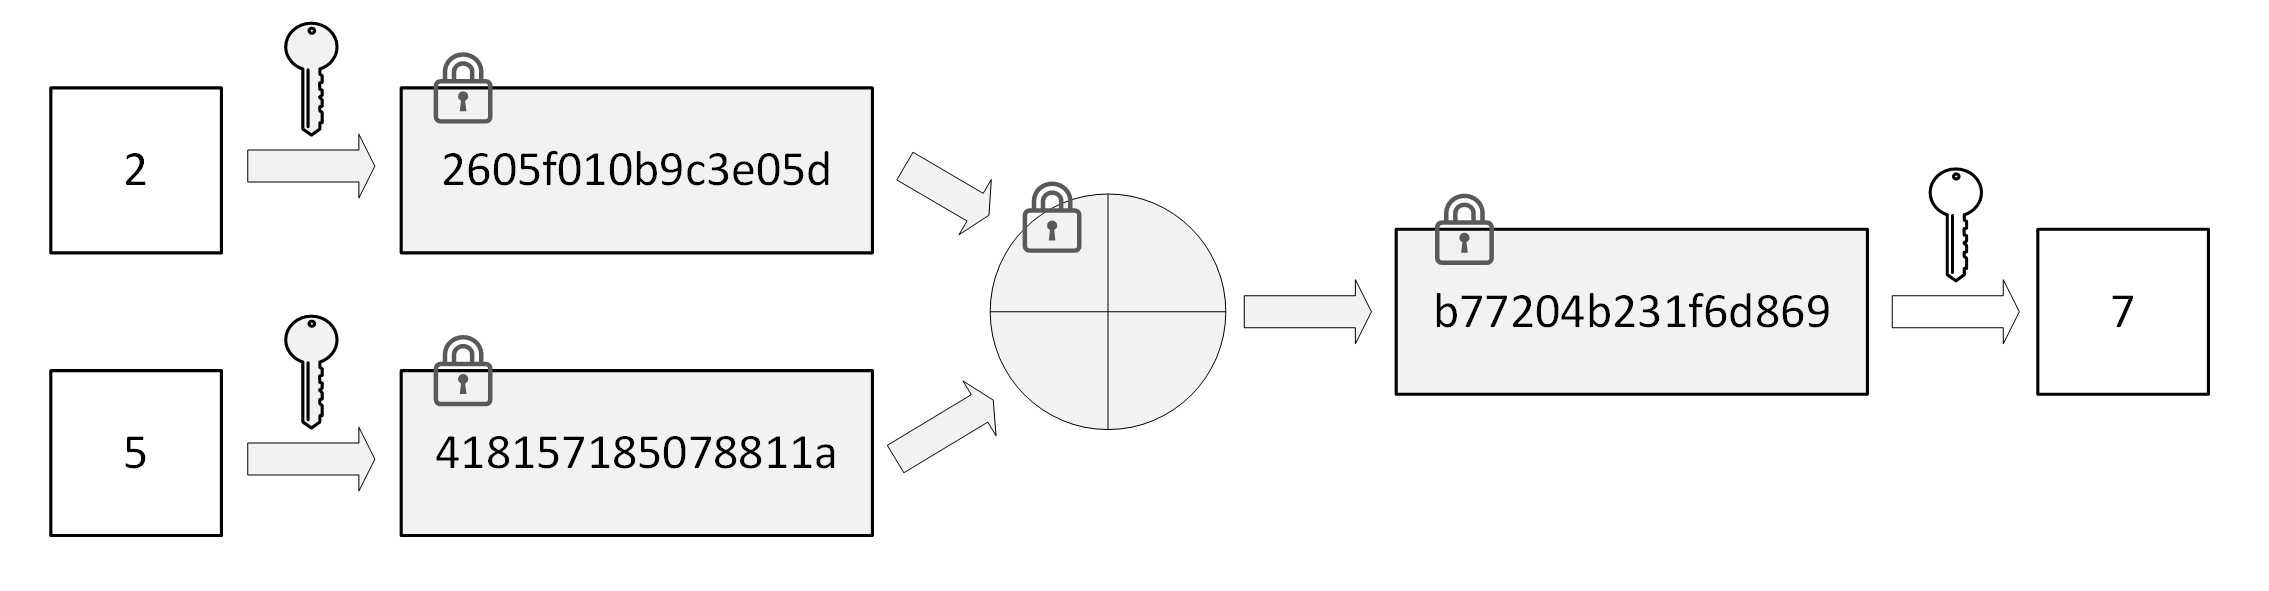
\includegraphics[width=\linewidth]{img/he.png}}
% 	\caption{Example of a homomorphic encryption operation directly on encrypted data. Gray shade indicates public key and encrypted data, while white shade represents plaintexts and secret key.}
% 	\label{fig:he}
% \end{figure}

\subsection{Data-oblivious programming}

{\it Data-oblivious computation} is a type of computation where the input data does not influence the behavior of the program. Under ``behavior'' we imply execution branching or memory access. 
Operations performed on encrypted data have to be in a data-oblivious form since ciphertexts are never decrypted, therefore the program is not capable of making decisions based on their plaintext values. In some fields, this property is also termed as {\it constant-time programming}, and has also been used for protecting against side-channel analysis.

% Consider a simple function calculating Fibonacci numbers in Listing~\ref{list:fibo}

Consider a simple function in Listing~\ref{list:fibo}. The iterations are interrupted once the index {\tt i} reaches the input value \texttt{in}. Assume that computation is now protected so the inputs and outputs must remain encrypted. Since variable {\tt in} cannot participate in any decisions to interrupt iterations, it must be processed in a data-oblivious way. We replace the interrupt condition with a multiplexer accumulator {\tt r} and introduce a fixed number of iterations {\tt max\_iter} not depending on the input, as shown in Listing~\ref{list:fibdo}. The number of iterations should exceed the input index, otherwise the accumulator will not reach the input index and will not get updated. The program shown in Listing~\ref{list:fibdo} works in constant time regardless of the input.

% To do that, we replace the interrupt condition with a multiplexer accumulator
% In this case, the number of iterations should exceed the input index,
\begin{figure}
%\scriptsize
\begin{minipage}{\linewidth}
\begin{lstlisting}[language=C++, caption={Simple Fibonacci function.
% \hspace{1cm} \mbox{}
}, style=mystyle, label=list:fibo, 
% xrightmargin=-0.12\linewidth,
% linewidth=0.96\linewidth
]
int fibonacci(int in)
{
    int i=0, a=0, b=1;
    while( i++ != in )
    {
        std::swap(a,b);
        a += b;
    }
    return a;
}
\end{lstlisting}
\end{minipage}
% \vspace{\lstbspace}
\vspace{-0.1in}
\end{figure}

\begin{figure}
%\scriptsize
\begin{minipage}{\linewidth}
\begin{lstlisting}[language=C++, caption={Data-oblivious Fibonacci function.
% \hspace{-0.05cm} \mbox{}
}, style=mystyle, label=list:fibdo,
% xrightmargin=-0.12\linewidth,
%linewidth=0.96\linewidth
]
int fibonacci(int in)
{
    int i=0, a=0, b=1;
    int r=0;
    int max_iter = 10;
    while( max_iter-- )
    {
        r += (i++ == in) * a;
        std::swap(a,b);
        a += b;
    }
    return r;
}
\end{lstlisting}
\end{minipage}
% \vspace{\lstbspace}
\vspace{-0.2in}
\end{figure}


Changing a program to its data-oblivious form is not trivial. This unavoidable requirement reflects the fundamental property of computation where data is never decrypted, which is the case for all FHE computation. This constraint can affect usability, as existing algorithms may need modifications to be converted to a data-oblivious version.\footnote{Computer-assisted program transformation to data-oblivious variants is an active topic of research, focusing currently on domain-specific languages and compilers \cite{alchemy,fact}.} 
Moreover, it affects practicality too, as fixed iteration upper bounds, introduce performance degradation.

% Moreover, it affects practicality too, as fixed iteration upper bounds, as shown in the example above, introduce performance degradation.

% \subsection{FHE schemes}\label{ss:fheschemes}

% Since the discovery of Fully Homomorphic Encryption~\cite{gentry2009thesis}, various FHE schemes have been released, each focusing on improving different features and functionalities. Popular schemes include BGV (Brakerski-Gentry-Vaikuntanathan) \cite{BGV_ref}, BFV (Brakerski/Fan-Vercauteren) \cite{brakerski2012fully,fan2012somewhatmisc}, CKKS (Cheon-Kim-Kim-Song) \cite{CKKS_ref, cheon2018bootstrapping}, and GSW (Gentry-Sahai-Waters) \cite{GSW_ref}. 

% \noindent {\bf BGV} is an FHE scheme based on the Ring Learning With Errors (RLWE) problem operating over polynomial rings of the form $\mathbb{Z}[X]/(X^{2^n}+1)$. It is
% naturally leveled meaning that without {\it bootstrapping} it allows evaluating a certain number of additions and multiplications on encrypted data, before a predefined {\it noise budget} is consumed.
% BGV encodes plaintext data as coefficients of a polynomial by defining special rules for polynomial addition, as well as multiplication defined as polynomial multiplication modulo a fixed irreducible polynomial. 
% This scheme requires two special operations to support ciphertext multiplication, namely {\it modulus switching} -- a ciphertext rescaling operation, and {\it relinearization} -- restoring the structure of a ciphertext as two sets of coefficients. 
% Given the ability to add and multiply encrypted data, it is possible to define arbitrary computation using either Boolean circuits (arithmetic modulo~2) or more general arithmetic circuits. 
% To address the noise budget limitation, BGV supports Gentry's bootstrapping theorem, which effectively allows resetting the ciphertext noise by homomorphically evaluating a special noise-refreshing circuit \cite{gentry2009fully}. BGV with bootstrapping support has been implemented in the HElib library \cite{githeli_bootstrap}.

% \noindent {\bf BFV} is the next major FHE scheme that introduces two optimizations for relinearization operations that require smaller key sizes and can enable faster performance. 
% BFV, unlike BGV, supports scale-invariant operations; so it does not require any modulus switching throughout the processing of encrypted data. Moreover, BFV is based on modular arithmetic with addition, subtraction, and multiplication support, and the plaintext modulus is usually a large number ($>2^{16}$) \cite{cryptonets, sealpir}. Like BGV, BFV also supports bootstrapping and can perpetually reduce ciphertext noise during computation. BFV without bootstrapping support has been implemented in Microsoft SEAL \cite{seal} and Palisade \cite{palisade} libraries.

% \noindent {\bf CKKS} is the first FHE cryptosystem for approximate arithmetic over complex numbers. CKKS is also based on RLWE. It encodes plaintext data into polynomials, and its modulus switching corresponds to a rounding operation of the encrypted values. Approximate arithmetic is beneficial for encrypted applications that operate on non-integer values, such as neural networks. CKKS has been implemented as part of HElib, Palisade, and SEAL libraries, as well as in the HEANN library, which is specifically developed to support fixed-point FHE arithmetic~\cite{heaan}.

% \noindent {\bf GSW} introduces another approach, called approximate eigenvector method, where the encryption key is an eigenvector of a ciphertext represented as a matrix. This approach enables defining a LWE-based cryptosystem that does not require expensive relinearization operations, and still supports bootstrapping to allow unlimited additions and multiplications of ciphertexts. GSW is the basis for the TFHE scheme \cite{chillotti2016faster} and the FHEW scheme \cite{ducas2015fhew}, both of which define homomorphic Boolean gates with bootstrapping, and allow processing of any Boolean circuit on FHE encryptions of bits (i.e., bit-level arithmetic).

\subsection{FHE Batching}
The FHE batching technique offers the ability to pack several plaintexts into ``slots'' within a single ciphertext. This feature is supported by some FHE schemes, and in practice  enables parallel processing of plaintexts, which are part of the same ciphertext (in a Single Instruction Multiple Data (SIMD) style)~\cite{batching}. Notably, such SIMD processing enables significant performance improvements for algorithms with parallel computation properties.
Each ciphertext variable is effectively a vector of values and any unary or binary operation has the effect of array operations on all elements of these vectors. Using batching, integral data types naturally have arrays of bit values inside each bit of the variable, and gate operations on each separate bit have the effect of the gate operation on all bit values.
BGV, BFV, and CKKS all support batching which enables parallel processing of encrypted vectors of data.

% \vspace{-0.4cm}

% and in practice  enables parallel processing of plaintexts, since they are all part of the same ciphertext
\section{Proposed Bridging Methodology}\label{s:bridging}

We define new data types to abstract the low-level complexity of the encryption scheme and Boolean circuits.
This is possible by extending the  E3 framework \cite{e3eprint}, which is one level of abstraction above FHE libraries and enables portability of code across different libraries.
% \vspace{-0.4cm}
\subsection{Modular and bit-level arithmetic}\label{ss:modcom}

Some FHE schemes define arithmetic addition, subtraction, and multiplication on numeric rings, but not other arithmetic such as division or comparison. While some applications may not require any other operation, a programmer is accustomed to having all programming operations available in their programs.
For example, the C++ statement "{\tt{}if(a<b)c+=a}" and its corresponding data-oblivious form: "{\tt{}c+=(a<b)*a}", cannot be evaluated with an FHE scheme where the comparison operation is not defined.
Notably, addition, subtraction, and multiplication on integers is an incomplete set of arithmetic operations; for instance, the comparison operation cannot be reduced to these three operations. However, when operating on bits, the same set of operations is universal, having addition and subtraction correspond to logical \texttt{XOR} and multiplication to logical \texttt{AND}.

\eee\ solves this problem by allowing the programmer to use data types constructed out of sequences of encrypted bits. Indeed, as the least possible requirement to the computing capacity, an FHE scheme must be able to evaluate the logic \texttt{NAND} (or \texttt{NOR}) gate on ciphertexts, since this elementary function is sufficient for universal computation. 
In this way, the variables in the expression "{\tt{}c+=(a<b)*a}" are defined as \emph{integral types} where all three operations (comparison, multiplication, and addition) are performed using bit-level arithmetic circuits. We call this computation {\it bit-level arithmetic}, as opposed to the natively provided {\it modular arithmetic}, where addition and multiplication are performed directly on ciphertexts.

The transition from modular to bit-level arithmetic is straightforward: Since
the encrypted bit values are limited to 0 and~1, logic gates, such as \texttt{AND}, \texttt{XOR}, \texttt{NOT}, etc, can be expressed via the following expressions:
\vspace{-0.2cm}
\begin{equation*}\label{eq:logic}
\begin{split}
x \ \texttt{AND} \ y = xy,& \qquad x \ \texttt{NAND} \ y = 1-xy \\
x \ \texttt{OR} \ y = x+y-xy,& \qquad x \ \texttt{NOR} \ y = 1-(x \ \texttt{OR} \ y) \\
x \ \texttt{XOR} \ y = x+y-2xy,& \qquad x \ \texttt{XNOR} \ y = 1-(x \ \texttt{XOR} \ y) \\
 \texttt{NOT} \ x = 1-x,& \qquad \texttt{MUX}(x,y,z) = x(y-z)+z, \\
\end{split}
\end{equation*}

\noindent where \texttt{MUX} is the multiplexer operation (as in {$x$?$y$:$z$}). The set of values $\{0,1\}$ is closed under the above set of expressions. 
In this paper, we use the term \emph{homomorphic gates} to describe logic gates operating on encrypted bits. Given these homomorphic gates, higher level operations (comparison, addition, multiplication) can be built using standard combinational arithmetic circuit design, which allows to perform any programming operation, i.e. giving the full spectrum of C++ arithmetic. Gate equations simplify for plaintext modulo $2$; e.g. XOR gate does not require multiplication, as \mbox{$x \ \texttt{XOR} \ y = x+y \bmod 2$}.

\innersection{Data types}
We define three data types for bit-level arithmetic, \secuint, \secint, and \secbool, and one for modular arithmetic, \secmod. 
A \secuint\ or \secint\ variable is an array of ciphertexts, each encrypting either zero or one. \secuint\ is comparable to \texttt{unsigned int}, while \secint\ corresponds to \texttt{int}.
The third type is \secbool, which is a type derived from \secuint\texttt{<1>}. It is the secure equivalent of \texttt{bool}.
For modular arithmetic, there is only the native type, which operates modulo the plaintext modulus. We call this type \secmod.

With bit-level arithmetic, we can express programs with operations not supported by modular arithmetic.
Listing~\ref{list:fibs} demonstrates the transition from plaintext computation to secure computation: Integer variables are declared with the secure type \secuint; the rest of the code remains the same.
%\footnote{\secuint\ is the secure equivalent of \texttt{unsigned int}. We discuss signed integers later.} Note that the type is parameterized with the size. 
In encrypted computation, increasing the number of bits of integral types can lead to a dramatic increase in performance overhead.
For this reason, we define the bit size as a template specialization.
% As experimental results demonstrate, even 1 bit can make significant difference in performance, affecting the practicality dimension. 
Explicit size declaration can be found in functional programming languages, so the programmer may already be familiar with this practice.
In the example of Listing~\ref{list:fibs}, all variables are 8 bits (lines 3, 4).

The postfix {\tt{}\_E} after each constant provides encrypted values used in variable initialization of integral type variables.
% The configuration file with the specifications of the encryption defines the type name and postfix used for constants in the program.
\eee\ automatically encrypts and replaces the plaintext constants with their encrypted representations, so the final binary does not have information about the initial values used in the program. 

\begin{figure}
%\scriptsize
\begin{minipage}{\linewidth}
\begin{lstlisting}[language=C++, caption={Secure version of Fibonacci function. Type \secuint\ behaves as native {\tt unsigned int}.
% \hspace{-1.40cm} \mbox{}
}, style=mystyle, label=list:fibs,
% xrightmargin=-0.12\linewidth,
% linewidth=0.96\linewidth
]
SecureUint<8> fibonacci(SecureUint<8> in)
{
    SecureUint<8> i=_0_E, a=_0_E, b=_1_E;
    SecureUint<8> r=_0_E;
    int max_iter = 10;
    while( max_iter-- )
    {
        r += (i++ == in) * a;
        std::swap(a,b);
        a += b;
    }
    return r;
}
\end{lstlisting}

\vspace{-0.5cm} 

% \vspace{0.2in}

% \begin{lstlisting}[language=C++, caption={An outline example of \secint\ definition.
% % \hspace{-1.40cm} \mbox{}
% }, style=mystyle, label=list:ciro,
% % xrightmargin=-0.12\linewidth,
% % linewidth=0.96\linewidth
% ]
% template <int Size> class SecureUint{ ... };
% constexpr std::string operator""_E
%   (unsigned long long int x){ ... }
% \end{lstlisting}
\end{minipage}
% \vspace{\lstbspace}
% \vspace{-0.8cm}
\end{figure}



\subsection{Bridging modular and bit-level arithmetic}\label{ss:bridging}

Declaring variables with a protected integral type and using solely bit-level arithmetic as in Listing~\ref{list:fibs} has a potential drawback: When an FHE scheme provides fast modular arithmetic operations, the usage of circuits operating on separate bits is slow. This paper brings the  idea of 
\textit{Bridging} - mixing both modular and bit-level arithmetic in one program with the ability to convert variables from one type to the other. %integral type to modular.
Some variables can be declared using a protected type supporting only modular arithmetic, while others with another secure type supporting bit-level arithmetic. In bridging mode, a type of bit-level arithmetic declares a conversion function into a type of modular arithmetic, and vice-versa.
In all cases, the encryption of the two different C++ types must share the same FHE keys, which is ensured by our proposed methodology and framework. 

\subsubsection{\secuint\ to \secmod{}}\label{sss:secuint2secmod}

For performance reasons, it is desirable to execute the entire computation in modular arithmetic, since it is much faster than bit-level. If however, a program requires an operation not supported in modular arithmetic (e.g., comparison), then, without Bridging, the whole program must perform all computations using bit-level arithmetic, severely degrading performance. 
In effect, Bridging enables the isolation of the parts of the computation requiring bit-level arithmetic.
For example, the expression "{\tt{}c+=(a<b)*a}" can use bit-level arithmetic for the comparison only.
The variables required by the comparison (i.e., \texttt{a} and \texttt{b}) must be of integral type. Nevertheless, the operands of the multiplication can be cast to our modular type, allowing multiplication and addition to be executed in modular arithmetic, resulting in a variable {\tt{}c} of modular type.

\input{list/fib_e3_mixed.tex}

Listing~\ref{list:fibm} demonstrates the code of the Fibonacci function of Listing~\ref{list:fibs} with \emph{Bridged} arithmetic: Only the input \texttt{in} and counter \texttt{i} are declared as integral type \secuint{}, while the others are replaced with the faster \secmod\ type. 
Line 8 does implicit conversion from \secuint\ to \secmod;
in this way, bit-level multiplication (which is slow) is not executed. Instead, only the native (much faster) multiplication of ciphertexts is needed.
Specifically, the comparison between {\tt i} and {\tt in} is the slowest operation in the program, and its result is one encrypted bit which can naturally be casted to \secmod, since the set $\{0,1\}$ is a subset of the plaintext range.
The operation for casting an integral type (bit-level) into modular (FHE native) is a summation of the encrypted bits of the integral type. 
In fact, the binary representation of a value $X$ can be reorganized by {\it Horner's scheme} in a set of additions over its $s$ bits $x_i$:
\begin{equation*}
\begin{split}
X & = 2^{s-1}x_{s-1} +2^{s-2}x_{s-2} + ... + 2x_1+x_0 = \\
& =(...((x_{s-1})\cdot 2+x_{s-2})\cdot 2+...+x_1)\cdot 2+x_0
\end{split}
\end{equation*}

Evaluating the right hand side of the above equation yields the value corresponding to the bit sequence. This evaluation is an efficient way to convert a program variable of type \secuint{} into a \secmod{} value.
Listing~\ref{list:secuint2secmod} shows the C++ implementation of such casting.
We emphasize that this conversion requires no ciphertext multiplications, only additions. Specifically, $2 \cdot (s - 1)$ ciphertext additions with a maximum additive depth of $s-1$, where $s$ is the number of encrypted bits.

\input{list/SecureUint_to_SecureMod}
\input{list/SecureInt_to_SecureMod}

Line 8 of Listing~\ref{list:fibm} does implicit conversion of \secbool{} to \secmod{}. Note that \secbool\ is a derived class from \secuint\texttt{<1>}. To observe a more complex scenario, consider the expression "{\tt{}c+=(a==b)*a}" that actually requires conversion of \secuint{}.
Comparison between \texttt{a} and \texttt{b} must be evaluated in bit-level. This implies that types of \texttt{a} and \texttt{b} must be \secuint{}. The comparison is done on a bit-by-bit manner using homomorphic gates following the gate equations described in Section \ref{ss:modcom}.
The gates correspond to normal logic gates, but operating on ciphertexts instead of ordinary bits. The result of the comparison is one encrypted bit represented by type \secbool.
Multiplication between a \secbool\ and a \secuint\ is evaluated as a multiplexer operation with $s$ \texttt{AND} gates, where $s$ is the number of encrypted bits in the \secuint\ variable, resulting in a \secuint{} type.
The type of variable \texttt{c} can be chosen as \secmod{}. The addition in the expression is then performed on variables of \secmod{} and \secuint{} types: "{\tt{}c=c+t}", where "{\tt{}t=(a==b)*a}". Implicit conversion evokes our function of Listing \ref{list:secuint2secmod} from the constructor of \secmod{} type out of \secuint{}.
Then the addition operation follows on two variables, both of the \secmod{} type.

It should be noted that all these conversions and evaluations are done obliviously to the user and do not require special attention; the user writes only "{\tt{}c+=(a==b)*a}".
A more efficient way to perform this computation is to explicitly convert argument \texttt{a}  in this expression to \secmod. In such case, the multiplication is done in modular arithmetic which is around $s$ times faster than a multiplication between \secbool{} and \secuint{} (and many more times faster than multiplying two \secuint{}s).\footnote{The exact speed-up compared to multiplying two \secuint s depends on the variables' bit size.} The corresponding expression becomes \mbox{"{\tt{}c+=(a==b)*\secmod(a)}"}.
Same way as above, the constructor calls the conversion function (Listing~\ref{list:secuint2secmod}), this time one step earlier - before the multiplication - resulting in having a larger portion of the computation in modular arithmetic, hence improving the performance.
It it worth noting that while there is automatic conversion from \secuint\ to \secmod, it is the programmer's task to define each variable's type and, in some cases, call conversion explicitly for better performance.

\subsubsection{\secint\ to \secmod{}}\label{sss:secint2secmod}

So far, we have discussed unsigned numbers. However, bit-level arithmetic also supports signed numbers following the two's complement arithmetic.
On the other hand, modular arithmetic only supports numbers in $\mathbb{Z}_t$, where $t$ is the plaintext modulus.
Nevertheless, it is possible to emulate negative numbers in modular arithmetic in the programmer's domain as in Cryptoleq \cite{cryptoleq}, where lower values are considered positive and large values are interpreted as negative numbers.
In this case, the conversion from a signed bit-level arithmetic type \secint\ to \secmod\ is defined as:
\begin{equation}
  X=\begin{cases}
    t - 2^s + \sum_{i=0}^{s-1}{(2^i \cdot x_i)}, & \text{if $x<0$}.\\
    \sum_{i=0}^{s-1}{(2^i \cdot x_i)}, & \text{otherwise}.
  \end{cases}
\end{equation}
where $s$ is the number of bits and $x_i$ is the bit of $x$ at position $i$. The condition $x < 0$ is determined by the most significant bit of $x$; thus, we can use it as a multiplexer between the two cases.
Listing \ref{list:secint2secmod} presents the algorithm for converting a \secint\ into a \secmod. First, the \secint\ is interpreted as a \secuint\ (line 4). In line 5, this value is converted into a \secmod\ using the algorithm of Listing \ref{list:secuint2secmod}.
Then in line 7, we perform the subtraction of plaintexts $t$ and \texttt{max} (i.e. $2^s$), and then do a ciphertext addition with the \secmod\ variable \texttt{pos}. At this point, we have generated two \secmod\ variables: \texttt{pos}, representing the value in case it is positive, and \texttt{neg} containing the value in case it is a negative number. This totals $2s - 1$ ciphertext additions with a additive depth of $s$.
Finally, we select between \texttt{neg} and \texttt{pos} using the most significant bit of the \secint\ input (lines 8-9). If the bit is one, it means it is a negative number; thus, we select \texttt{neg}; otherwise, we select \texttt{pos}.
For selection we need ciphertext multiplications.
The entire conversion from \secint\ to \secmod\ requires two ciphertext multiplications and $2s + 1$ ciphertext additions with a multiplicative depth equal to one.
By comparing Listings \ref{list:secuint2secmod} and \ref{list:secint2secmod}, we can see that converting signed numbers to \secmod\ is less efficient than converting unsigned numbers to \secmod. Furthermore, $t$ must be large enough ($t \geq 2^s$) to accommodate the converted value.

% \innersection{Why not signed and unsigned \secmod{}} \secmod{} types can only participate in addition, subtraction, and multiplication operations. The values of this type are elements of the corresponding mathematical ring. The programmer can choose to interpret a subset of the number space as negative, but there would be no difference in these computations. For this reason, there is no differentiation between the signed and unsigned versions for \secmod{} type.
\subsubsection{\secmod\ to \secuint{}}\label{sss:secmod2secuint}
\vspace{-0.2cm}
Conversion from \secmod\ to \secuint\ is theoretically possible using the expression:
\vspace{-0.2cm}
\begin{equation}\label{eq:secmod2secuint}
    \vspace{-0.1cm}
    X = \sum_{i=1}^{t-1}(i \cdot \secbool(1 - (x-i)^{t-1}))
\end{equation}
where $x$ is the \secmod\ variable to be converted, $t$ is the plaintext modulus and is prime, $i$ is a \secuint\ counter, and $X$ is the resulting \secuint. Due to the properties of modular arithmetic and the parameters used in homomorphic encryption, the exponentiation to $t-1$ results in zero in case the base is zero, and one otherwise. When $i = x$, the expression in the summation results in $i$, while in all other cases it will result in zero, since $1 - (x-i)^{t-1} = 0 \ \forall \ i \ne x$.
% Breaking down Eq. \ref{eq:secmod2secuint}:
% \begin{enumerate}
%     \item The \secuint\ $i$ is automatically cast to \secmod\ in $x-i$ before the exponentiation, resulting in a subtraction between two \secmod{}s.
%     \item The exponentiation of the \secmod\ $x-i$ to the integer $t-1$ results in a \secmod\ variable containing either the encryption of zero or one.
%     \item The result of the exponentiation is negated by subtracting it from one. At this point, we have the encryption of one in case $x = i$ and zero otherwise stored in a \secmod\ variable. In order to avoid automatically casting $i$ to \secmod\ in the multiplication, we must first reinterpret the partial result as \secbool.
%     \item We multiply the \secuint\ $i$ by the \secbool\ value resulting in a \secuint\ equal to $i$ or zero. We remark that a \secbool-\secuint\ multiplication is evaluated as a multiplexer operation.
%     \item We repeat this process for all $i \in [1,t)$, adding the resulting values. The final result is a \secuint\ equal to $x$ since there is only one $i$ that is equal to $x$.
% \end{enumerate}

An implementation of the fast exponentiation algorithm is presented in Listing \ref{list:pow}. The number of multiplications is given by $\floor{\log_2{e}} + \omega(e) - 1$ and the multiplicative depth is $\ceil{\log_2{e}}$, where $e$ is the exponent and $\omega(\cdot)$ is a function that calculates the Hamming weight. The conversion from \secmod\ to \secuint\ can exploit this property of the exponentiation to $t-1$ resulting in zero or one to create an equality function, where the equality function is given by $1 - (x-i)^{t-1}$. With this information, we can build a linear search to find the \secuint\ $i$ that is equal to the \secmod\ $x$ using the result of the equality as a selector. Listing \ref{list:secmod2secuint} presents the algorithm that performs this conversion.
The number of multiplications is given by $t \cdot (s + \floor{\log_2{(t-1)}} + \omega(t-1) - 1)$, while the multiplicative depth is equal to $\ceil{\log_2{(t-1)}} + 1$.
One can notice that this algorithm is only practical for small plaintext moduli $t$. Once $t$ becomes large, the linear search makes it impractical. Since \secmod\ requires a large $t$ for it to be useful, this conversion should not be used in practice and should be avoided, as later presented and discussed in Section~\ref{ss:conversion}.

\input{list/pow}
\input{list/SecureMod_to_SecureUint}
% \input{table/table_sec3-3}
% \input{table/table_generalization}


\subsubsection{\secmod\ to \secint{}}\label{sss:secmod2secint}

Conversion from \secmod\ to \secint\ is possible by applying Eq. \ref{eq:secmod2secint} to the result of Eq. \ref{eq:secmod2secuint}:
\begin{equation}\label{eq:secmod2secint}
    Y = (1 - X_{s-1}) \cdot X + X_{s-1} \cdot (2^s - t + X)
\end{equation}
$X$ is the result of Eq. \ref{eq:secmod2secuint}, $Y$ is the \secint\ output, $s$ is the number of encrypted bits in $X$ and $Y$, $t$ is the plaintext modulus, and $2^s \geq t$.
Listing \ref{list:secmod2secint} shows the algorithm for this conversion. It leverages the conversion described in Listing \ref{list:secmod2secuint} and adjusts for the sign.
This algorithm requires $2 \cdot t \cdot (s + \floor{\log_2{(t-1)}} + \omega(t-1) - 1)+2$ multiplications with a multiplicative depth of $\ceil{\log_2{(t-1)}} + 2$.

\input{list/SecureMod_to_SecureInt}
% \subsection{Discussion on practical use of bridging}\label{ss:discussion}

In Table \ref{tab:conversion}, we present the conversion cost from \secuint\ and \secint\ to \secmod, and vice-versa, considering several bit sizes ($s \in \{4, 7, 8, 16\}$) and plaintext moduli ($t \in \{2^4+1, 2^7+1, 2^{16}+1\}$)\review{, while Table \ref{tab:general} shows the general terms}.
Converting from \secuint\ to \secmod\ does not use ciphertext multiplications; therefore it is very efficient.
A conversion from \secint\ to \secmod\ needs only two multiplications, the cost of which is amortized since expensive bit-level arithmetic multiplications are avoided.

On the other hand, conversion from \secmod\ to \secuint\ is very costly.
A ciphertext multiplication in Microsoft SEAL BFV with polynomial degree $n = 2^{15}$ takes around 0.41s using the experimental setup described in Section \ref{ss:setup}, and the smallest plaintext modulus for $n = 2^{15}$ that enables batching is $t = 2^{16}+1$.
In this scenario, a conversion from \secmod\ to \secuint\ would take more than a week, while converting from \secmod\ to \secint\ takes nearly double that time.
Practical times for the conversion could be achieved only for very small plaintext moduli, in the order of $2^4+1$. Such small moduli is meaningful only with the BGV encryption scheme, which supports much smaller plaintext moduli with batching.
Considering comparable time for ciphertext multiplication, it would be possible to convert from \secmod\ to \secuint\ under one minute for 4 bits of precision ($s = 4$ and $t = 2^4+1$), and in around 12 minutes for 7 bits of precision ($s = 7$ and $t = 2^7+1$).


\section{Experimental Results}\label{s:results}

\subsection{Overview and setup}\label{ss:setup}

We evaluate bridging using three sets of experiments:
\begin{enumerate}
    \item Conversion from \secuint\ and \secint\ to \secmod, and vice-versa, using different bit sizes.
    \item Performance comparison of bridging and bit-level arithmetic using synthetic benchmarks.
    \item Case study analysis using one real-world FHE application.
\end{enumerate}

% The results presented in Sections \ref{ss:conversion} and \ref{ss:benchmarks} were collected using a single thread of an Intel i7-4790 CPU @ 3.60GHz with 16 GB of RAM, 64 GB of swap area, running Ubuntu 18.04.5, with GCC 9.4.0.\footnote{Due to memory requirements, the setup for the genotype imputation case study differs and is defined locally in the section.} We use the E3 framework (commit \#9fb718f) with SEAL 3.3.2 as underlying FHE library, and BFV as the encryption scheme. We set the encryption parameters as: polynomial degree $n = 2^{15}$, as it provides the largest noise budget for encrypted computation, and plaintext modulus $t = 2^{16}+1$, as this is the smallest $t$ that enables batching for the chosen $n$. While a smaller $t$ would provide less noisy homomorphic operations, virtually all practical FHE applications rely on efficient utilization of batching. Nevertheless, although $t=2$ does not enable batching on BFV, we also test it on the benchmarks (Section \ref{ss:benchmarks}) since some homomorphic gates are simpler in modulo 2. The remaining parameters are automatically defined by SEAL given the required security level of 128 bits.

% As this application has much higher memory requirements compared to the previous experiments, we ran the experiments on an Intel Xeon Silver 4214R CPU @ 2.40GHz with 24 cores and 1 TB of memory running on RHEL 7.9. We use the same version of E3 and Microsoft SEAL as in the other experiments with GCC 7.3.1.
The results presented in Section \ref{s:results} were collected using a single thread (Sections \ref{ss:conversion} and \ref{ss:benchmarks}) and 24 threads (Section \ref{sss:genotype}) of an Intel Xeon Silver 4214R CPU @ 2.40GHz with 24 cores and 1 TB of memory running on RHEL 7.9, with GCC 7.3.1. We use the E3 framework (commit \#9fb718f) with SEAL 3.3.2 \cite{seal} as underlying FHE library, and BFV as the encryption scheme. We set the encryption parameters as: polynomial degree $n = 2^{15}$, as it provides the largest noise budget for encrypted computation, and plaintext modulus $t = 2^{16}+1$, as this is the smallest $t$ that enables batching for the chosen $n$. While a smaller $t$ would provide less noisy homomorphic operations, virtually all practical FHE applications rely on efficient utilization of batching. Nevertheless, although $t=2$ does not enable batching on BFV, we also test it on the benchmarks (Section \ref{ss:benchmarks}) since some homomorphic gates are simpler in modulo 2. The remaining parameters are automatically defined by SEAL given the required security level of 128 bits.
\subsection{Conversion}\label{ss:conversion}

Fig. \ref{fig:tosecmod} presents the conversion latency time from \secuint\ and \secint\ to \secmod\ for different bit sizes following the algorithms of Listings \ref{list:secuint2secmod} and \ref{list:secint2secmod}. The number of multiplications for \secuint\ and \secint\ stays constant at 0 and 2, while the multiplicative depth is 0 and 1, respectively, for all bit sizes. 
\iffalse As discussed in Section \ref{ss:bridging}, converting from \secint\ is slower than converting from \secuint\ because a \secint\ to \secmod\ conversion uses two ciphertext multiplications to account for the sign \fi . As expected, conversion from both \secuint\ and \secint\ becomes slower for larger bit sizes due to the larger number of additions required. The slowdown is the same for both types. It is less noticeable for \secint\ due the log-scale graph and the fact that the multiplications dominate the \secint\ latency time.

\begin{figure}[t]
	\centering
    \frame{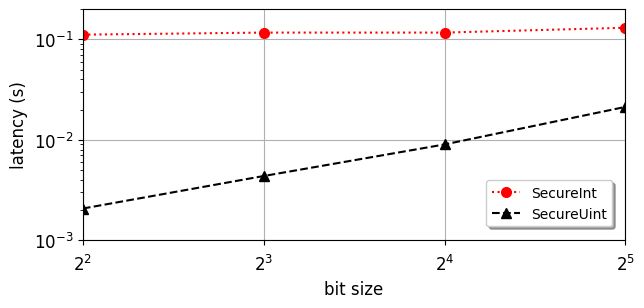
\includegraphics[width=\linewidth]{img/toSecureMod.png}}
	\caption{Conversion latency time from \secuint\ and \secint\ to \secmod\ for different bit sizes. Throughput is up to $n=2^{15}$ times faster since a ciphertext fits $n$ plaintexts.}
	\label{fig:tosecmod}
	\vspace{-0.6cm} 
\end{figure}

We also evaluate the conversion latency time from \secmod\ to \secuint/\secint\ using the algorithms presented in Listings \ref{list:secmod2secuint} and \ref{list:secmod2secint} with different plaintext moduli and bit sizes ($s = \{4, 8, 16, 32\}$). Fig.~\ref{fig:fromsecmod} summarizes the findings.
The results are what we expect from analysing the algorithms in Listings \ref{list:secmod2secuint} and \ref{list:secmod2secint}: When converting from \secmod\ to \secuint, the latency increases linearly to the bit size due to the operation on line 11 of Listing \ref{list:secmod2secuint}. Nevertheless, the dominant factor is the plaintext modulus $t$. A minor logarithmic effect comes from the exponentiation function (line 10) where the number of multiplications increases, while a major linear effect comes from the larger number of iterations in the \texttt{for} loop (line 7).
The conversion from \secmod\ to \secint\ (Listing \ref{list:secmod2secint}) takes roughly twice the time since it consists of two calls to the \secmod\ to \secuint\ conversion (lines 4 and 8) plus two multiplications (line 11).

\begin{figure}[t]
	\centering
    \frame{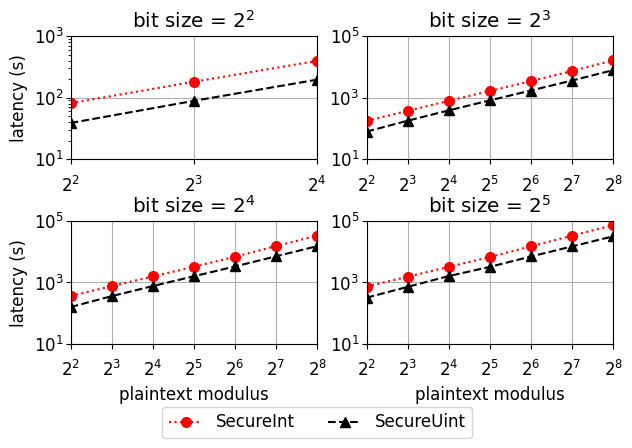
\includegraphics[width=\linewidth]{img/fromSecureMod.png}}
	\caption{Conversion latency time from \secmod\ to \secuint\ and \secint\ for different plaintext moduli and bit sizes.}
	\label{fig:fromsecmod}
	\vspace{-0.5cm}
\end{figure}



% \innersection{Insights}
% The results show that the conversion from bit-level to modular arithmetic is fast and can be used in practice. Meanwhile, converting from modular to bit-level arithmetic has borderline practical times only for very small plaintext moduli. With an small increase in the plaintext modulus, it quickly becomes prohibitive.

\subsection{Benchmarks}\label{ss:benchmarks}

In order to evaluate different execution modes (bit-level arithmetic and bridging), we use six data-oblivious benchmarks, some of which were adapted from the TERMinator Suite \cite{terminator}. \iffalse , while others were included based on their use in FHE applications. \fi These benchmarks are developed to be data-oblivious and manipulate sets of encrypted variables adjusted to $\{4, 8, 16\}$-bit size.
The algorithms are: (FIB) Fibonacci, an additive-intensive algorithm, (LOG) Logistic Regression, where the data must be capped before inference, (MAX) Maximum, commonly used as non-linear function in ML applications, (MUX) Multiplexer, a simple operation similar to the ternary operator that replaces branch conditions on encrypted data, (PKS) Private Keyword Search, which searches privately for an item in a list or database, and (SOR) Sort, a sorting algorithm with low multiplicative depth, designed for FHE.

% The algorithms are: (FIB) Fibonacci, an additive-intensive algorithm that we use as example in this manuscript, (LOG) Logistic Regression, where the data must be capped before inference, (MAX) Maximum, commonly used as non-linear function in machine learning applications, (MUX) Multiplexer, a simple operation similar to the ternary operator that replaces branch conditions on encrypted data, (PKS) Private Keyword Search, which searches privately for an item in a list or database, and (SOR) Sort, a sorting algorithm with low multiplicative depth specifically designed for FHE.
% The source code of all benchmarks with and without bridging is available in the Appendix.

\begin{figure}[t]
    % \vspace{-0.2cm}
	\centering
    \frame{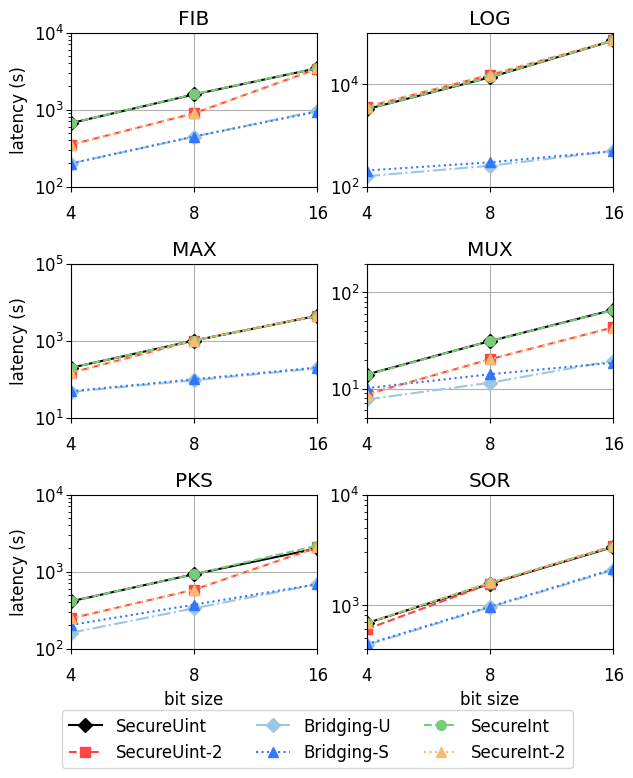
\includegraphics[width=\linewidth]{img/cases_latency.png}}
	\caption{Latency time for six benchmarks\iffalse using \secuint, \secint, unsigned and signed bridging, \texttt{Bridging-U} and \texttt{Bridging-S}, respectively,\fi with $t=2^{16}+1$. \iffalse In addition, we evaluate the benchmarks using \secuint\ and \secint\ with $t=2$ (postfix \texttt{-2}). \fi}
	\label{fig:benchmarks}
	\vspace{-0.4cm} 
\end{figure}

\innersection{Effect of plaintext modulus} Although $t=2$ does not enable batching in BFV, and therefore, it would not be used in practice, we compare it against the smallest plaintext modulus that enables batching ($t=2^{16}+1$) for $n=2^{15}$. The plaintext modulus does not affect the latency time to execute a homomorphic operation, but some homomorphic gates simplify in modulo 2 (e.g. XOR), as we discuss in Section \ref{ss:modcom}. Thus, a Boolean circuit used in bit-level arithmetic should have lower latency for $t=2$ if it contains XOR or XNOR gates. In Fig. \ref{fig:benchmarks}, we can see that in fact some applications are faster in modulo 2 (\texttt{SecureUint-2} and \texttt{SecureInt-2} for unsigned and signed bit-level arithmetic with $t=2$). MUX is the simplest benchmark, containing in bit-level arithmetic one equality, two \secbool-\secuint\ multiplications (or \secbool-\secint\ for signed numbers), one negation, and one addition. A \secbool-\secuint\ multiplication is entirely composed of XOR gates, and around half of the gates in the equality are XOR or XNOR. These operations are mainly responsible for the speed-up. 

% We have a similar situation for FIB and PKS, however here there are relatively fewer \secbool-\secuint\ multiplications and more additions, diminishing the effect of operating in modulo 2. The other benchmarks are much more complex applications and we noticed no difference in latency time between $t=2$ and $t=2^{16}+1$.

\innersection{Bit-level arithmetic vs bridging} Fig. \ref{fig:benchmarks} presents the latency time comparison between bit-level arithmetic and bridging. Regarding unsigned numbers (\secuint\ vs \texttt{Bridging-U}), results show that bridging outperforms bit-level arithmetic for all benchmarks and bit sizes. For some applications, like SOR, the performance improvement is limited (around 60\% speed-up). This happens because this algorithm requires many non-native operations (comparisons) in most stages. Only in the last part of the algorithm bridging can be employed, since using bridging before would require the inefficient conversion from \secmod\ to \secuint\ in order to execute the latter comparisons. Conversely, the logistic regression benefits a lot from using bridging with a speed-up of more than two orders of magnitude. This is possible because the non-native operations required by the filtering function are executed first. Therefore, at the filtering stage it is already possible to employ bridging and perform the remaining computation using the faster modular arithmetic.

\innersection{Signed numbers} Also in Fig. \ref{fig:benchmarks} we compare how bridging behaves with signed numbers. \iffalse In general, the extra conversion time required for signed numbers has little effect in the latency since the application uses significantly more multiplications compared to all the conversions. \fi We can see some degradation in PKS (4 bits) and MUX (4 and 8 bits). In PKS, there is conversion from \secint\ to \secmod\ in every iteration of the loop. The slowest operation in the loop is the comparison. This comparison operation is faster for smaller circuits (4 bits); therefore, the proportional latency of the two ciphertext multiplications required for the \secint\ to \secmod\ conversion is higher. For larger circuits, the comparison becomes more costly, thus, amortizing the conversion cost.

% Regarding MUX, it is a very simple function. It consists only of a comparison followed by a selection of one of two items. The explanation is similar to PKS, but the signed conversion has a higher impact in the latency time because there are two conversions instead of one in this algorithm.

\begin{figure}[t]
    % \vspace{-0.2cm}
	\centering
    \frame{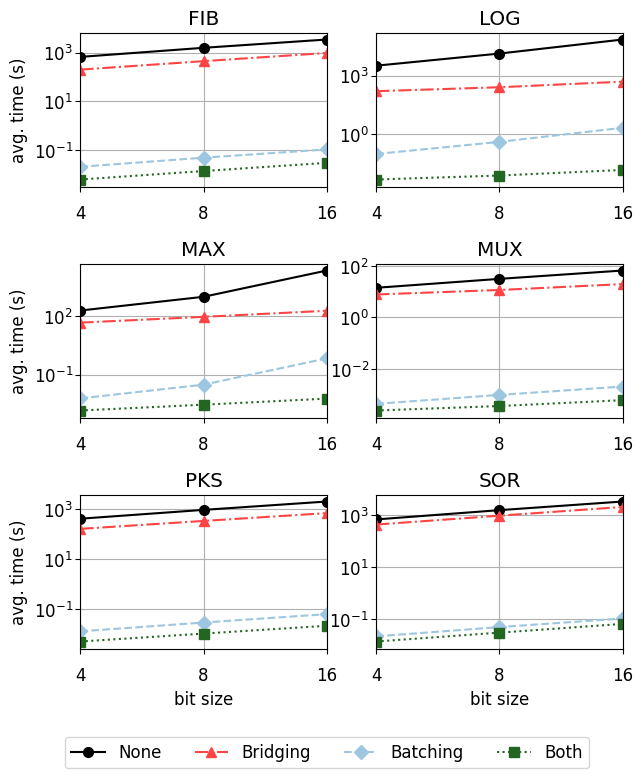
\includegraphics[width=\linewidth]{img/batching.png}}
	\caption{Average execution time for six benchmarks. \iffalse using and four cases: \texttt{None}: without bridging and batching, \texttt{Bridging}: with bridging only, \texttt{Batching}: with batching only, and \texttt{Both}: with both bridging and batching.\fi}
	\label{fig:batching}
	\vspace{-0.4cm} 
\end{figure}



\innersection{Bridging can be used with batching} Batching is a powerful technique used in FHE to pack many plaintexts into a ciphertext. The number of plaintexts that can be packed into a ciphertext is equal to the polynomial degree ($n = 2^{15}$ in our case). Although carefully crafted algorithms using batching and rotations can reduce program latency, the main benefit of batching is increased throughput, since it is possible to process $n$ plaintexts at once. Bridging on the other hand always reduces latency, and consequently improves throughput.
Bridging is a technique independent of batching and both can be used in tandem.
In Fig. \ref{fig:batching} we present the average execution time ($\text{latency} / \text{\# plaintexts packed}$) for six benchmarks and four cases: no batching and no bridging (\texttt{None}), bridging-only (\texttt{Bridging}), batching-only (\texttt{Batching}), and batching and bridging together (\texttt{Both}).
As expected, the throughput improvement provided by batching is impressive. However, for this technique to be used at its fullest, it is necessary to fill all ciphertext slots with plaintexts, which is the case with embarrassingly parallel workload. If the load is less than $n$, the performance will degrade.
Bridging does not suffer from this problem since it focuses on reducing the latency.
Nevertheless, bridging can be used in combination with batching. In this case, the speed-up of both techniques is added, leading to an even faster runtime (acceleration by more than 6 orders of magnitude (LOG)).

\innersection{Insights}
Bridging demonstrates substantial performance improvement for algorithms that allow mixing \secuint{} and \secmod{}, while in the worst case, bridging is equivalent to bit-level arithmetic. \iffalse This would happen if all outputs of a program come out from non-native operations. \fi
The comparison heavy SOR benefits less from bridging since these operations occur throughout the program and near the output, which precludes using the \secmod{} type in an earlier stage. On the contrary the benchmarks containing non-native operations near the beginning exhibit more significant performance improvements (MAX, FIB, PKS).
\iffalse At first glance, the MAX algorithm looks similar to SOR. However, some subtle differences in the \texttt{selection} function allow us to use bridging much earlier in the program; in fact, near the beginning of the application, leading to a much more noticeable performance improvement. 
FIB, and PKS have comparisons in all iterations, but since these comparisons are at the beginning of each iteration, bridging provides substantial performance improvements. \fi
Bridging benefits are maximized when non-native operations (e.g. comparisons) are at the beginning of the computation and the remaining of the computation can be done in modular arithmetic. The non-native operation would require the whole computation to work on bit-level arithmetic, but with bridging it becomes much faster since only the non-native operations are performed with \secuint, while the remaining run using \secmod. This is demonstrated by our logistic regression benchmark, which provides more than two orders of magnitude (precisely 143 times) of performance improvement.

% Finally, it is possible to combine bridging with batching for further performance improvement since both techniques are orthogonal to each other. It should be noted that this performance improvement is tightly connected to the parallelization capabilities of the workload. Nevertheless, results show that some benchmarks, when \emph{both} batching and bridging are combined, can be accelerated by more than 6 orders of magnitude (LOG).

\vspace{-0.1cm}
% \subsection{Case studies}\label{ss:cases}

% \subsubsection{URL denylisting}
\label{ss:url}
\input{list/pmt_sort}

We evaluate the performance improvements provided by bridging using a URL denylisting application as a case study \cite{urldenylist}.
The application implements a Private Membership Test (PMT) protocol, a common cryptographic building block for privacy-preserving applications.
Its main operation is checking if an element is part of a database without revealing information about the element.
In this scenario, the server hosting the database is semi-trusted (honest-but-curious).

URL denylisting is the process where a URL is being checked against a known database of malicious URLs; if there is a match, the access to the website is blocked. URL denylisting can be used in conjunction with URL rewriting to protect against e-mail phishing attacks. In other words, when an email comes to the company server, its URLs are being replaced by a redirection to the service provider site, which checks whether the link is malicious or not. If it is benign, the user is automatically forwarded to the webpage. While this (supposedly) protects against phishing attacks, it introduces a huge privacy problem, since the company hosting the service can clearly see which links the users are visiting, and can potentially sell the data to other parties. 

The PMT protocol we evaluate here is composed of two main phases: setup and query. In the setup phase, the database is converted into a format that enables fast queries. The query phase is simply checking if a particular element is part of the database.
While queries are fast, the setup is expensive since it uses comparison operations. As mentioned in the previous sections, comparisons require bit-level arithmetic, leading to execution times of more than a day for databases with millions of entries. Implementing a faster setup protocol is therefore critical to the practicality of the application. 

The setup protocol is composed of three main stages: 1) The server database containing the list of malicious URLs is converted into a Bloom filter \cite{bloomfilter}. The server then informs the size of this Bloom filter $m$ to the client. 2) In the next step, the client creates a list with random permutations of \mbox{$\ceil{ {m}/({n \cdot \floor{\log_{2}{t}}} ) }$} unique integers, where $m$ is the size of the Bloom filter, $n$ is the polynomial degree, and $t$ is the plaintext modulus. The client encrypts the list with its public key and sends to the server. 3) Finally, the server runs a particular homomorphic algorithm that sorts the Bloom filter into a way only known to the client. This produces an encrypted Bloom filter in this particular order.

Out of the three stages in the setup, only the third one operates homomorphically on encrypted data. Therefore, we implemented the third stage of the setup protocol using bridging and compared its performance against the bit-level arithmetic implementation.
As shown in Fig. \ref{fig:application}, bridging provides approximately one order of magnitude of performance improvement for this application, reducing the setup time for databases with one million entries to less than three hours, instead of more than a day when bit-level arithmetic is exclusively used.

\begin{figure}[t]
	\centering
    \frame{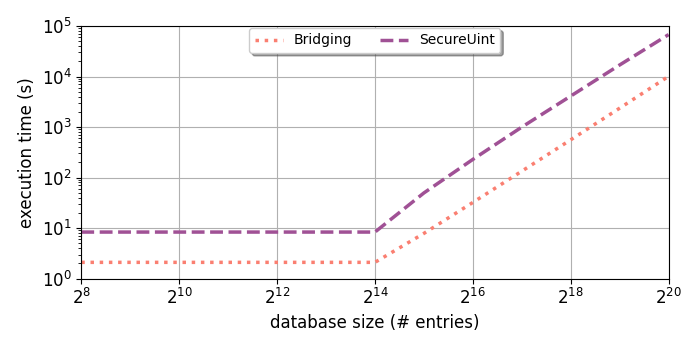
\includegraphics[width=\linewidth]{img/application.png}}
	\caption{Execution time of the setup protocol of a URL denylisting application \cite{urldenylist} implementing the Private Membership Test.}
	\label{fig:application}
\end{figure}

This performance improvement is enabled with just a few tweaks to the sort algorithm.
Consider Listing \ref{list:pmt_sort} presenting this algorithm as an example of modifications required to enable bridged computation.
Function \texttt{sort} reorders the items of a Bloom filter in a sequence known only to the client using encrypted variable \texttt{order}. It creates a list of plaintext indices according to the protocol (lines 10-23), compares homomorphically with the encrypted list of unique permutations sent by the client (variable \texttt{order}), and composes the encrypted Bloom filter \texttt{efilter} with values in this particular order (lines 25-42).

The homomorphic operations start after line 24. There are only a few necessary changes to the algorithm: 1) In lines 1, 26, and 31 we change the return and variable types from \texttt{vector<\secuint<S>{}>} to \texttt{vector<\secmod>}, and 2) in line 35, we cast the \secbool\ type to \secmod, so the subsequent multiplication is done using modular arithmetic.
In bit-level arithmetic it is faster to cast the \texttt{vector<int>} to \secuint\ and multiply by a \secbool, since it results in a \secbool-\secuint\ multiplication instead of a \secuint-\texttt{vector<int>} multiplication. Nevertheless, with bridging it is faster to cast the \secbool\ to \secmod, instead of \texttt{vector<int>}, because \secmod-\texttt{vector<int>} multiplication is faster and less noisy than \secmod-\secmod\ multiplication.
As can be seen in Fig. \ref{fig:application}, Bridging unlocks {\it one order of magnitude} performance improvement, and it only requires minor changes to the source code.

% \subsubsection{Genotype imputation}\label{sss:genotype}
\subsection{Case-study: Genotype imputation}\label{sss:genotype}

Genotype imputation is the process of filling missing information in DNA sequencing with the use of statistical methods. \iffalse Due to the computer-intensive nature of the task, cloud servers are a natural platform for processing the data. Furthermore, privacy requirements of medical information make solutions using homomorphic encryption desirable. \fi P-Impute \cite{GURSOY2021} converts an inefficient statistical model based on correlation of similar individuals %\footnote{The similarity of individuals is determined based on matching single-nucleotide polymorphisms (SNPs) in proximity to the missing SNP.}
into a Private Information Retrieval (PIR) problem, which has efficient solutions in FHE, using the BFV encryption scheme. In this section, we discuss the performance of p-Impute without (\secuint) and with bridging taking into consideration the multiplicative depth for defining more efficient encryption parameters. Batching is used to fit $n$ plaintexts into a ciphertext.

% As this application has much higher memory requirements compared to the previous experiments, we ran the experiments on an Intel Xeon Silver 4214R CPU @ 2.40GHz with 24 cores and 1 TB of memory running on RHEL 7.9. We use the same version of E3 and Microsoft SEAL as in the other experiments with GCC 7.3.1.
We set each run to use 24 threads and report the query time, i.e., the time performing encrypted computation, and the number of ciphertext additions, multiplications, and subtractions in Table \ref{tab:nops}. We use the same plaintext modulus as in the other experiments ($t = 2^{16}+1$), but we vary the polynomial degree ($n \in \{2^{13}, 2^{14}, 2^{15}\}$) in order to evaluate the extra performance improvement provided by bridging for requiring a lower multiplicative depth.
Without bridging, we were only able to run with $n = 2^{15}$, since lower polynomial degrees do not provide enough noise budget to run the application without bootstrapping. %\footnote{Bootstrapping is not supported by Microsoft SEAL library. Accounting for noise growth is commonly tasked to the programmer in FHE applications.}
With bridging, we were able to reduce $n$ to $2^{13}$ without corrupting the result.
As $n$ reduces, the number of batching slots in a ciphertext reduces since it is equal to the polynomial degree. However, the reduction in latency for the homomorphic operation compensates for the reduction in slots. Experimental results show that when $n$ is halved, the latency of the ciphertext multiplication reduces by at least 4 times, and can be amplified depending on the behavior of cache memories. \iffalse This effect can be even greater due to effects related to cache memories.  Therefore, reducing the polynomial degree is always desirable.\fi Consequently, one halving of $n$ increases throughput by at least 2x and reduces latency by 4x.

For the same polynomial degree ($n = 2^{15}$), bridging is around 6.82x faster than bit-level arithmetic. This is due to the reduced number of operations on encrypted data, as one can see in Table \ref{tab:nops}.
Nevertheless, bridging requires less noise budget to operate, which allows us to use smaller polynomial degrees. In the fastest case, bridging has the throughput improved by 62.2x, while the latency reduces by around 249 times.
\vspace{-0.1cm}
\input{table/nops}

\section{Discussion}\label{s:related_work}

\noindent {\bf Polynomial degree:}
We compare bridging with other accelerations of homomorphic computation at the programming level.
% \vspace{-0.5cm}
As we show in Section \ref{sss:genotype}, the polynomial degree affects the performance and noise budget. A smaller polynomial degree makes operations a few times faster. At the same time, it reduces the noise budget, allowing fewer computations before data corruption or bootstrapping. It also reduces the number of plaintexts that can be packed in a ciphertext when batching. Nevertheless, the performance improvement from a smaller polynomial degree outweighs the fewer batching slots in the ciphertexts.
% The best option is to use the smallest polynomial degree that does not corrupt the ciphertext. 

\noindent {\bf Batching} enables SIMD usage of ciphertexts \cite{batching}. It can provide several orders of magnitude performance improvement for SIMD-compatible applications, however not all FHE schemes support it \cite{chillotti2016faster,ducas2015fhew}. Due to its significant computational benefits, batching should always be used where possible. \iffalse if the target application is compatible with it. \fi

% Unfortunately, not all FHE schemes support batching (e.g., TFHE \cite{chillotti2016faster} and FHEW \cite{ducas2015fhew}). The ones that do, such as BGV \cite{BGV_ref} or BFV \cite{fan2012somewhatmisc}, support it only for some specific encryption parameters, which may not be the most noise efficient parameters for the target application.
% In any case, due to its significant performance benefits, batching should always be used if the target application is compatible with it.

\noindent {\bf Bridging} makes possible to use the comprehensive bit-level arithmetic and the fast modular arithmetic in the same program. It increases the expressivity of programs previously limited to modular arithmetic, and improves performance of complex programs implemented using bit-level arithmetic. At the same time, it reduces noise, since the depth of the datapath is shorter due to fewer homomorphic operations being executed, which may enable using a smaller polynomial degree, further improving performance.
Therefore, the performance improvement provided by bridging comes from two factors: 1) Reduced number of homomorphic operations since Boolean circuits performing additions and multiplications in bit-level arithmetic are replaced by a single operation (native addition or multiplication), and 2) reduced multiplicative depth, since when Boolean circuits are replaced by a single instruction, the multiplicative depth reduces. This reduces the noise budget required by the application, enabling the use of a smaller polynomial degree, further improving performance.
In addition, bridging is independent of encryption parameters, apart from the plaintext modulus which should not be too small. This makes bridging perfectly compatible with batching and any polynomial degree.

% \noindent {\bf Class of programs benefiting from bridging}:
% FHE itself is already introducing restrictions on the class of programs that can be practically used with FHE-encrypted data. Within the subset of applications that have demonstrated such potential, the algorithms that benefit the most from bridging should have all non-native operations at the beginning of computation with the remaining computation using only native operations. This applies well to the algorithms involving data selection followed by computation on selected data. Therefore, examples of such classes of programs are 1) membership tests (case study 1 - URL denylist), 2) information retrieval, 3) set intersections, and 4) keyword search (case study 2 - genotype imputation). On the other hand, algorithms having non-native operations throughout the computation or near its output would not benefit from bridging. This is the case for sorting algorithms, which are mostly comparisons, and some block ciphers algorithms that are heavy on bit-wise operations.
\section{Conclusions}\label{s:conclusions}

In this work, we presented a new methodology combining universal bit-level arithmetic and faster modular arithmetic computation, dubbed \emph{bridging}, to accelerate applications using fully homomorphic encryption. Experiments demonstrate significant performance improvements when using both bridging and batching modes. Bridging by itself can offer several orders of magnitude performance improvement, depending on the type of application. \iffalse In the worst case, bridging offers no performance improvement, but also no performance degradation. Applications with complex operations requiring bit-level arithmetic at the beginning of execution followed by long operations on modular arithmetic are the ones that benefit the most from bridging. \fi In the benchmark evaluation, bridging improved performance by more than 2 orders, and 6 orders of magnitude when combined with batching. 
Furthermore, the case-study private genotype imputation became two orders of magnitude faster due to reduced number of homomorphic operations and multiplicative depth, allowing us to use more efficient encryption parameters.

\section*{Resources}

Bridging has been integrated with the E3 framework and is available on github.com/momalab/e3 from commit \#88a323f.

%%
%% The next two lines define the bibliography style to be used, and
%% the bibliography file.
\bibliographystyle{ACM-Reference-Format}
\bibliography{reference}

% \vspace{-0.8cm}
\section*{Appendix}
\vspace{-0.2cm}
We include in this appendix the codes referent to the benchmarks used in \ref{ss:benchmarks}. The codes presented feature \secint, but the code using \secuint\ is similar.

\vspace{-0.1cm}
\begin{figure}[h]

%\scriptsize
% \vbox to 600pt {
\noindent\begin{minipage}{.50\textwidth}
\begin{lstlisting}[language=C++,
caption={Private Keyword Search using bit-level arithmetic.},
style=mystyle, label=list:pks_bit,
%framexrightmargin=-37pt,
% xleftmargin=0.4cm,
% xrightmargin=-0.12\linewidth,
% linewidth=0.88\linewidth
]
template <int S> SecureInt<S>
pks(vector<SecureInt<S>> v, SecureInt<S> k)
{
    vector<SecureInt<S>> r;
    for (size_t i=0; i < v.size(); i++)
    {
        auto eq = i == k;
        auto sel = eq * v[i];
        r.push_back(sel);
    }
    return sum(r);
}
\end{lstlisting}
\end{minipage}
% \vspace{\lstbspace}


% }
\end{figure}

\vspace{-1.3cm}
\begin{figure}[h]
%\scriptsize
\noindent\begin{minipage}{.50\textwidth}
\begin{lstlisting}[language=C++,
caption={Private Keyword Search with bridging.},
style=mystyle, label=list:pks_bridge,
%framexrightmargin=-37pt,
% xleftmargin=0.4cm,
% xrightmargin=-0.12\linewidth,
% linewidth=0.88\linewidth
]
template <int S> SecureMod
pks(vector<SecureInt<S>> v, SecureInt<S> k)
{
    vector<SecureMod> r;
    for (size_t i=0; i < v.size(); i++)
    {
        auto eq = i == k;
        auto sel = eq * SecureMod(v[i]);
        r.push_back(sel);
    }
    return sum(r);
}
\end{lstlisting}
\end{minipage}
% \vspace{\lstbspace}
\end{figure}


% \begin{figure}[t]
% %\scriptsize
% \noindent\begin{minipage}{.45\textwidth}
% \begin{lstlisting}[language=C++,
% caption={Private Keyword Search with bridging.},
% style=mystyle, label=list:pks_bit,
% %framexrightmargin=-37pt,
% % xleftmargin=0.4cm,
% % xrightmargin=-0.12\linewidth,
% % linewidth=0.88\linewidth
% ]
% template <int S> SecureMod
% pks(vector<SecureInt<S>> v, SecureInt<S> k)
% {
%     vector<SecureMod> r;
%     for (size_t i=0; i < v.size(); i++)
%     {
%         auto eq = i == k;
%         auto sel = eq * SecureMod(v[i]);
%         r.push_back(sel);
%     }
%     return sum(r);
% }
% \end{lstlisting}
% \end{minipage}
% % \vspace{\lstbspace}
% \end{figure}




\begin{figure}[t]
%\scriptsize
\begin{minipage}{\linewidth}
\begin{lstlisting}[language=C++,
caption={Logistic regression with data filtering using bit-level arithmetic.},
style=mystyle, label=list:log_bit,
%framexrightmargin=-37pt,
% xleftmargin=0.4cm,
% xrightmargin=-0.12\linewidth,
% linewidth=0.88\linewidth
]
template <class T> vector<vector<T>>
appendCol(vector<vector<T>> m, T value)
{
  for (auto & v : m) v.push_back(value);
  return m;
}

template <int S>
vector<vector<SecureInt<S>>>
filter(vector<vector<SecureInt<S>>> m,
  SecureInt<S> threshold, vector<int> pos)
{
  for (auto & idx : pos)
  {
    for (auto & v : m)
    {
      auto cond = v[idx] > threshold;
      v[idx] = cond * threshold
            + !cond * v[idx];
    }
  }
  return m;
}

template <int S>
vector<vector<SecureInt<S>>>
mm(vector<vector<SecureInt<S>>> a,
  vector<vector<SecureInt<S>>> b)
{
  auto n = a.size();
  auto m = b.size();
  auto p = b[0].size();
  vector<vector<SecureInt<S>>> c(n);
  for (size_t i=0; i<n; i++)
  {
    for (size_t j=0; j<p; j++)
    {
      vector<SecureInt<S>> t;
      for (size_t k=0; k<m; k++)
        t.push_back(a[i][k] * b[k][j]);
      c[i].push_back(sum(t));
    }
  }
  return c;
}

template <int S>
vector<vector<SecureInt<S>>>
logreg(vector<vector<SecureInt<S>>> inputs,
  vector<vector<SecureInt<S>>> weights,
  SecureInt<S> threshold, vector<int> pos)
{
  SecureInt<S> one = _1_E;
  filter(inputs, threshold, pos);
  auto inputsU = convert(inputs, one);
  appendCol(inputsU, one);
  return mm(inputsU, weights);
}
\end{lstlisting}
\end{minipage}
% \vspace{\lstbspace}
\end{figure}

\begin{figure}[b]
%\scriptsize
\begin{minipage}{\linewidth}
\begin{lstlisting}[language=C++,
caption={Logistic regression with data filtering using bridging.},
style=mystyle, label=list:log_bridge,
%framexrightmargin=-37pt,
% xleftmargin=0.4cm,
% xrightmargin=-0.12\linewidth,
% linewidth=0.88\linewidth
]
template <class T> vector<vector<T>>
appendCol(vector<vector<T>> m, T value)
{
  for (auto & v : m) v.push_back(value);
  return m;
}

template <int S>
vector<vector<SecureInt<S>>>
filter(vector<vector<SecureInt<S>>> m,
  SecureInt<S> threshold, vector<int> pos)
{
  for (auto & idx : pos)
  {
    for (auto & v : m)
    {
      auto cond = v[idx] > threshold;
      v[idx] = cond * threshold
            + !cond * v[idx];
    }
  }
  return m;
}


vector<vector<SecureMod>>
mm(vector<vector<SecureMod>> a,
  vector<vector<SecureMod>> b)
{
  auto n = a.size();
  auto m = b.size();
  auto p = b[0].size();
  vector<vector<SecureMod>> c(n);
  for (size_t i=0; i<n; i++)
  {
    for (size_t j=0; j<p; j++)
    {
      vector<SecureMod> t;
      for (size_t k=0; k<m; k++)
        t.push_back(a[i][k] * b[k][j]);
      c[i].push_back(sum(t));
    }
  }
  return c;
}

template <int S>
vector<vector<SecureMod>>
logreg(vector<vector<SecureInt<S>>> inputs,
  vector<vector<SecureMod>> weights,
  SecureInt<S> threshold, vector<int> pos)
{
  SecureMod one = _1_M;
  filter(inputs, threshold, pos);
  auto inputsU = convert(inputs, one);
  appendCol(inputsU, one);
  return mm(inputsU, weights);
}
\end{lstlisting}
\end{minipage}
% \vspace{\lstbspace}
\end{figure}


\begin{figure}[t]
%\scriptsize
\begin{minipage}{\linewidth}
\begin{lstlisting}[language=C++,
caption={Bit-level depth-optimized max function.},
style=mystyle, label=list:max_bit,
%framexrightmargin=-37pt,
% xleftmargin=0.4cm,
% xrightmargin=-0.12\linewidth,
% linewidth=0.88\linewidth
]









template <int S> vector<SecureInt<S>>
indices(vector<SecureInt<S>> v)
{
  int size = v.size();
  vector<SecureInt<S>> idx;
  vector<vector<SecureInt<S>>> m(size);
  for (int i=0; i < size; i++)
  {
    for (int j=i+1; j < size; j++)
    {
      auto cond = v[i] > v[j];
      m[i].push_back(SecureInt<S>(cond));
      m[j].push_back(SecureInt<S>(!cond));
    }
    idx.push_back(product(m[i]));
  }
  return idx;
}

template <int S> SecureInt<S>
select(vector<SecureInt<S>> idx,
  vector<SecureInt<S>> v)
{
  int size = v.size();
  vector<SecureInt<S>> r;
  for (int i=0; i < size; i++)
    r.push_back(idx[i] * v[i]);
  return sum(r);
}

template <int S> SecureInt<S>
max(vector<SecureInt<S>> v)
{
  return select(indices(v), v);
}

\end{lstlisting}
\end{minipage}
% \vspace{\lstbspace}
\end{figure}

\begin{figure}[t]
%\scriptsize
\begin{minipage}{\linewidth}
\begin{lstlisting}[language=C++,
caption={The multiplexer function using bit-level arithmetic.},
style=mystyle, label=list:mux_bit,
%framexrightmargin=-37pt,
% xleftmargin=0.4cm,
% xrightmargin=-0.12\linewidth,
% linewidth=0.88\linewidth
]
template <int S> SecureInt<S>
mux(SecureInt<S> input, SecureInt<S> item,
    SecureInt<S> t, SecureInt<S> f)
{
    auto cond = input == item;
    return cond * t
        + !cond * f;
}
\end{lstlisting}
\end{minipage}
% \vspace{\lstbspace}
\end{figure}

\begin{figure}[t]
%\scriptsize
\begin{minipage}{\linewidth}
\begin{lstlisting}[language=C++,
caption={Depth optimized max function with bridging.},
style=mystyle, label=list:max_bridge,
%framexrightmargin=-37pt,
% xleftmargin=0.4cm,
% xrightmargin=-0.12\linewidth,
% linewidth=0.88\linewidth
]
template <class T> vector<SecureMod>
convert(vector<T> v)
{
    vector<SecureMod> u;
    for (auto & e : v)
        u.push_back(SecureMod(e));
    return u;
}

template <int S> vector<SecureMod>
indices(vector<SecureInt<S>> v)
{
  int size = v.size();
  vector<SecureMod> idx;
  vector<vector<SecureMod>> m(size);
  for (int i=0; i < size; i++)
  {
    for (int j=i+1; j < size; j++)
    {
      auto cond = v[i] > v[j];
      m[i].push_back(SecureMod(cond));
      m[j].push_back(SecureMod(!cond));
    }
    idx.push_back(product(m[i]));
  }
  return idx;
}

SecureMod
select(vector<SecureMod> idx,
    vector<SecureMod> v)
{
  int size = v.size();
  vector<SecureMod> r;
  for (int i=0; i < size; i++)
    r.push_back(idx[i] * v[i]);
  return sum(r);
}

template <int S> SecureMod
max(vector<SecureInt<S>> v)
{
  return select(indices(v), convert(v));
}
\end{lstlisting}
\end{minipage}
% \vspace{\lstbspace}
\end{figure}

\begin{figure}[t]
%\scriptsize
\begin{minipage}{\linewidth}
\begin{lstlisting}[language=C++,
caption={The multiplexer function with bridging.},
style=mystyle, label=list:mux_bridge,
%framexrightmargin=-37pt,
% xleftmargin=0.4cm,
% xrightmargin=-0.12\linewidth,
% linewidth=0.88\linewidth
]
template <int S> SecureMod
mux(SecureInt<S> input, SecureInt<S> item,
    SecureInt<S> t, SecureInt<S> f)
{
    auto cond = input == item;
    return cond * SecureMod(t)
        + !cond * SecureMod(f);
}
\end{lstlisting}
\end{minipage}
% \vspace{\lstbspace}
\end{figure}


\begin{figure}[t]
%\scriptsize
\begin{minipage}{\linewidth}
\begin{lstlisting}[language=C++,
caption={Depth-optimized sorting algorithm using bit-level arithmetic.},
style=mystyle, label=list:sor_bit,
%framexrightmargin=-37pt,
% xleftmargin=0.4cm,
% xrightmargin=-0.12\linewidth,
% linewidth=0.88\linewidth
]









template <int S> vector<SecureInt<S>>
indices(vector<SecureInt<S>> v)
{
  int size = v.size();
  vector<SecureInt<S>> idx;
  vector<vector<SecureInt<S>>> m(size);
  for (int i=0; i < size; i++)
  {
    for (int j=i+1; j < size; j++)
    {
      auto cond = v[i] > v[j];
      m[i].push_back(SecureInt<S>(cond));
      m[j].push_back(SecureInt<S>(!cond));
    }
    idx.push_back(sum(m[i]));
  }
  return idx;
}

template <int S> vector<SecureInt<S>>
select(vector<SecureInt<S>> idx,
  vector<SecureInt<S>> v)
{
  int size = v.size();
  vector<SecureInt<S>> r;
  for (int i=0; i < size; i++)
  {
    vector<SecureInt<S>> t;
    for (int j=0; j < size; j++ )
      t.push_back((i == idx[j]) * v[j]);
    r.push_back(sum(t));
  }
  return r;
}

template <int S> vector<SecureInt<S>>
sort(vector<SecureInt<S>> v)
{
  return select(indices(v), v);
}

\end{lstlisting}
\end{minipage}
% \vspace{\lstbspace}
\end{figure}

\begin{figure}[t]
%\scriptsize
\begin{minipage}{\linewidth}
\begin{lstlisting}[language=C++,
caption={Depth-optimized sorting algorithm using bridging.},
style=mystyle, label=list:sor_bridge,
%framexrightmargin=-37pt,
% xleftmargin=0.4cm,
% xrightmargin=-0.12\linewidth,
% linewidth=0.88\linewidth
]
template <class T> vector<SecureMod>
convert(vector<T> v)
{
    vector<SecureMod> u;
    for (auto & e : v)
        u.push_back(SecureMod(e));
    return u;
}

template <int S> vector<SecureInt<S>>
indices(vector<SecureInt<S>> v)
{
  int size = v.size();
  vector<SecureInt<S>> idx;
  vector<vector<SecureInt<S>>> m(size);
  for (int i=0; i < size; i++)
  {
    for (int j=i+1; j < size; j++)
    {
      auto cond = v[i] > v[j];
      m[i].push_back(SecureInt<S>(cond));
      m[j].push_back(SecureInt<S>(!cond));
    }
    idx.push_back(sum(m[i]));
  }
  return idx;
}

template <int S> vector<SecureMod>
select(vector<SecureInt<S>> idx,
  vector<SecureMod> v)
{
  int size = v.size();
  vector<SecureMod> r;
  for (int i=0; i < size; i++)
  {
    vector<SecureMod> t;
    for (int j=0; j < size; j++ )
      t.push_back((i == idx[j]) * v[j]);
    r.push_back(sum(t));
  }
  return r;
}

template <int S> vector<SecureMod>
sort(vector<SecureInt<S>> & v)
{
  return select(indices(v), convert(v));
}


\end{lstlisting}
\end{minipage}
% \vspace{\lstbspace}
\end{figure}



\end{document}
\endinput
%%
%% End of file `sample-sigconf.tex'.

%%
%% The abstract is a short summary of the work to be presented in the
%% article.
\begin{abstract}
The dramatic increase of data breaches in modern computing platforms has emphasized that access control is not sufficient to protect sensitive user data. Recent advances in cryptography allow end-to-end processing of encrypted data without the need for decryption using Fully Homomorphic Encryption (FHE).
Such computation however, is still orders of magnitude slower than direct (unencrypted) computation. Depending on the underlying cryptographic scheme, FHE schemes can work natively either at bit-level using Boolean circuits, or over integers using modular arithmetic. Operations on integers are limited to addition/subtraction and multiplication. On the other hand, bit-level arithmetic is much more comprehensive allowing more operations, such as comparison and division. While modular arithmetic can emulate bit-level computation, there is a significant cost in performance.
In this work, we propose a novel method, dubbed \emph{bridging}, that blends faster and restricted modular computation with slower and comprehensive bit-level computation, making them both usable within the same application and with the same cryptographic scheme instantiation. We introduce and open source C++ types representing the two distinct arithmetic modes, offering the possibility to convert from one to the other.
Experimental results show that bridging modular and bit-level arithmetic computation can lead to 1-2 orders of magnitude performance improvement for tested synthetic benchmarks, as well as  one real-world FHE application: a genotype imputation case study.
\end{abstract}

% Bridging performance enhancement comes from two factors: 1) Reduced number of operations (especially ciphertext multiplications), and 2) Arithmetic circuits with smaller multiplicative depth, allowing more efficient encryption parameters with smaller polynomial degrees.

% % old abstract
% \begin{abstract}
% The dramatic increase of data breaches in modern computing platforms has emphasized that access control is not sufficient to protect sensitive user data. Recent advances in cryptography allow end-to-end processing of encrypted data without the need for decryption using Fully Homomorphic Encryption (FHE).
% Such computation however, is still orders of magnitude slower than direct (unencrypted) computation. Depending on the underlying cryptographic scheme, FHE schemes can work natively either at bit-level using Boolean circuits, or over integers using modular arithmetic. Operations on integers are limited to addition/subtraction and multiplication. On the other hand, bit-level arithmetic is much more comprehensive allowing more operations, such as comparison and division. While modular arithmetic can emulate bit-level computation, there is a significant cost in performance.
% In this work, we propose a novel method, dubbed \emph{bridging}, that blends faster and restricted modular computation with slower and comprehensive bit-level computation, making them both usable within the same application and with the same cryptographic scheme instantiation. We introduce and open source C++ types representing the two distinct arithmetic modes, offering the possibility to convert from one to the other.
% Experimental results show that bridging modular and bit-level arithmetic computation can lead to 1-2 orders of magnitude performance improvement for tested synthetic benchmarks, as well as  one real-world FHE application: a genotype imputation case study. Bridging performance enhancement comes from two factors: 1) Reduced number of operations (especially ciphertext multiplications), and 2) Arithmetic circuits with smaller multiplicative depth, allowing more efficient encryption parameters with smaller polynomial degrees.
% \end{abstract}


%%
%% The code below is generated by the tool at http://dl.acm.org/ccs.cfm.
%% Please copy and paste the code instead of the example below.
%%
\begin{CCSXML}
<ccs2012>
   <concept>
       <concept_id>10002978.10003022.10003028</concept_id>
       <concept_desc>Security and privacy~Domain-specific security and privacy architectures</concept_desc>
       <concept_significance>500</concept_significance>
       </concept>
 </ccs2012>
\end{CCSXML}

\ccsdesc[500]{Security and privacy~Domain-specific security and privacy architectures}

%%
%% Keywords. The author(s) should pick words that accurately describe
%% the work being presented. Separate the keywords with commas.
% \keywords{fully homomorphic encryption, privacy-preserving computation, modular arithmetic}
\keywords{fully homomorphic encryption, privacy-preserving computation}
\section{Preliminaries}\label{s:preliminaries}

\subsection{Homomorphic Encryption}

Homomorphic encryption is a special type of encryption that allows meaningful operations in the encrypted domain. Within homomorphic encryption, there are several types of encryption schemes. Partially Homomorphic Encryption (PHE) schemes support only one homomorphic operation over ciphertexts, usually either addition or multiplication. FHE schemes support two orthogonal operations, usually addition and multiplication, theoretically allowing Turing complete computation.

Operations on ciphertexts without decryption are possible using homomorphic functions. Suppose the homomorphic function F over ciphertexts $c_x$ and $c_y$ corresponds to plaintext operation $f$.
Let $f(m_x,m_y)$ denote a two-argument function on plaintexts $m_x$ and $m_y$; $\text{E}_k(m,r)$ denotes a probabilistic encryption function generated by a random sequence $k$ (key) that maps a plaintext $m$ to a set of ciphertexts $c$ depending on a probabilistic parameter $r$, and $\text{D}_k(c)$ denotes a deterministic decryption function corresponding to $\text{E}_k$ that maps ciphertext $c$ to the corresponding plaintext $m$. Then,
F is defined by the homomorphism of surjective
$\text{D}_k$:
\begin{equation*}
\text{D}_k\big(\text{F}(c_x,c_y)\big) = 
f\big(\text{D}_k(c_x), \text{D}_k(c_y)\big),
\end{equation*}
which converts into the
explicit composition over ciphertexts:
% which can be converted into the
% explicit composition over ciphertexts:
\begin{equation*}\label{e:chop}
\text{F}(c_x,c_y) = 
\text{E}_k\Big(f\big(\text{D}_k(c_x), \text{D}_k(c_y)\big),\text{H}(c_x,c_y)\Big)
\end{equation*}
where H is an arbitrary function generating the randomness value $r$ from the input ciphertexts. This expression establishes a functional requirement for F, which does not decrypt nor re-encrypt the data.

% for F; though F does not decrypt nor re-encrypt the data.

% Fig. \ref{fig:he} depicts an example of a homomorphic addition operation. Plaintexts $2$ and $5$ are encrypted with a public key, generating their respective ciphertexts. These ciphertexts are inputs to a function that operates directly on encrypted data and produces an encrypted output, which, when decrypted with the secret key, results in a plaintext equivalent to the addition of the input plaintexts.

% \begin{figure}[t]
% 	\centering
%     \frame{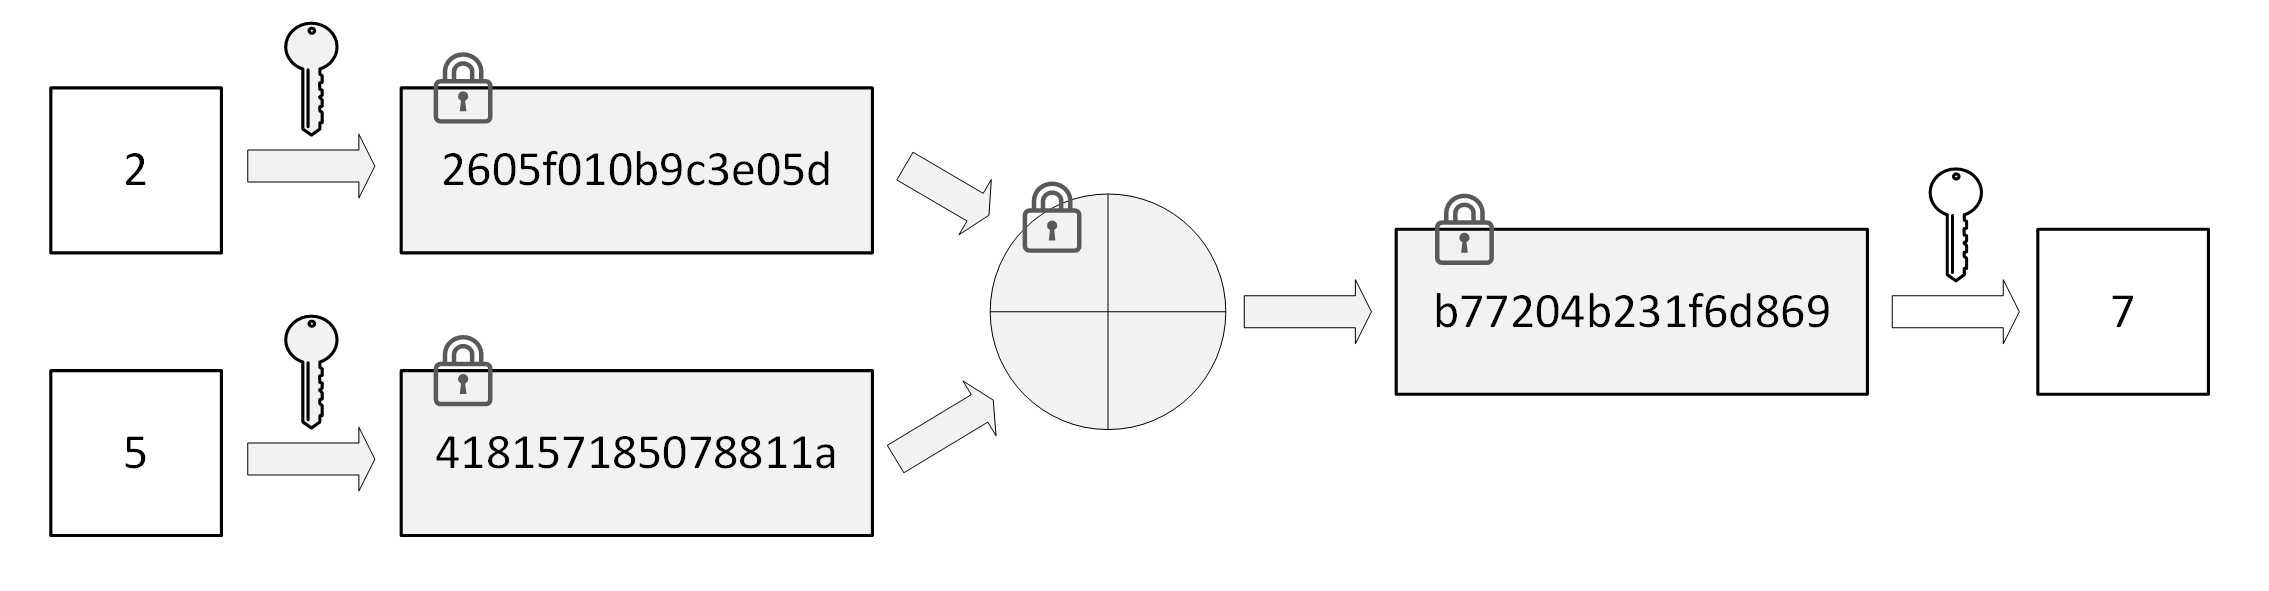
\includegraphics[width=\linewidth]{img/he.png}}
% 	\caption{Example of a homomorphic encryption operation directly on encrypted data. Gray shade indicates public key and encrypted data, while white shade represents plaintexts and secret key.}
% 	\label{fig:he}
% \end{figure}

\subsection{Data-oblivious programming}

{\it Data-oblivious computation} is a type of computation where the input data does not influence the behavior of the program. Under ``behavior'' we imply execution branching or memory access. 
Operations performed on encrypted data have to be in a data-oblivious form since ciphertexts are never decrypted, therefore the program is not capable of making decisions based on their plaintext values. In some fields, this property is also termed as {\it constant-time programming}, and has also been used for protecting against side-channel analysis.

% Consider a simple function calculating Fibonacci numbers in Listing~\ref{list:fibo}

Consider a simple function in Listing~\ref{list:fibo}. The iterations are interrupted once the index {\tt i} reaches the input value \texttt{in}. Assume that computation is now protected so the inputs and outputs must remain encrypted. Since variable {\tt in} cannot participate in any decisions to interrupt iterations, it must be processed in a data-oblivious way. We replace the interrupt condition with a multiplexer accumulator {\tt r} and introduce a fixed number of iterations {\tt max\_iter} not depending on the input, as shown in Listing~\ref{list:fibdo}. The number of iterations should exceed the input index, otherwise the accumulator will not reach the input index and will not get updated. The program shown in Listing~\ref{list:fibdo} works in constant time regardless of the input.

% To do that, we replace the interrupt condition with a multiplexer accumulator
% In this case, the number of iterations should exceed the input index,
\begin{figure}
%\scriptsize
\begin{minipage}{\linewidth}
\begin{lstlisting}[language=C++, caption={Simple Fibonacci function.
% \hspace{1cm} \mbox{}
}, style=mystyle, label=list:fibo, 
% xrightmargin=-0.12\linewidth,
% linewidth=0.96\linewidth
]
int fibonacci(int in)
{
    int i=0, a=0, b=1;
    while( i++ != in )
    {
        std::swap(a,b);
        a += b;
    }
    return a;
}
\end{lstlisting}
\end{minipage}
% \vspace{\lstbspace}
\vspace{-0.1in}
\end{figure}

\begin{figure}
%\scriptsize
\begin{minipage}{\linewidth}
\begin{lstlisting}[language=C++, caption={Data-oblivious Fibonacci function.
% \hspace{-0.05cm} \mbox{}
}, style=mystyle, label=list:fibdo,
% xrightmargin=-0.12\linewidth,
%linewidth=0.96\linewidth
]
int fibonacci(int in)
{
    int i=0, a=0, b=1;
    int r=0;
    int max_iter = 10;
    while( max_iter-- )
    {
        r += (i++ == in) * a;
        std::swap(a,b);
        a += b;
    }
    return r;
}
\end{lstlisting}
\end{minipage}
% \vspace{\lstbspace}
\vspace{-0.2in}
\end{figure}


Changing a program to its data-oblivious form is not trivial. This unavoidable requirement reflects the fundamental property of computation where data is never decrypted, which is the case for all FHE computation. This constraint can affect usability, as existing algorithms may need modifications to be converted to a data-oblivious version.\footnote{Computer-assisted program transformation to data-oblivious variants is an active topic of research, focusing currently on domain-specific languages and compilers \cite{alchemy,fact}.} 
Moreover, it affects practicality too, as fixed iteration upper bounds, introduce performance degradation.

% Moreover, it affects practicality too, as fixed iteration upper bounds, as shown in the example above, introduce performance degradation.

% \subsection{FHE schemes}\label{ss:fheschemes}

% Since the discovery of Fully Homomorphic Encryption~\cite{gentry2009thesis}, various FHE schemes have been released, each focusing on improving different features and functionalities. Popular schemes include BGV (Brakerski-Gentry-Vaikuntanathan) \cite{BGV_ref}, BFV (Brakerski/Fan-Vercauteren) \cite{brakerski2012fully,fan2012somewhatmisc}, CKKS (Cheon-Kim-Kim-Song) \cite{CKKS_ref, cheon2018bootstrapping}, and GSW (Gentry-Sahai-Waters) \cite{GSW_ref}. 

% \noindent {\bf BGV} is an FHE scheme based on the Ring Learning With Errors (RLWE) problem operating over polynomial rings of the form $\mathbb{Z}[X]/(X^{2^n}+1)$. It is
% naturally leveled meaning that without {\it bootstrapping} it allows evaluating a certain number of additions and multiplications on encrypted data, before a predefined {\it noise budget} is consumed.
% BGV encodes plaintext data as coefficients of a polynomial by defining special rules for polynomial addition, as well as multiplication defined as polynomial multiplication modulo a fixed irreducible polynomial. 
% This scheme requires two special operations to support ciphertext multiplication, namely {\it modulus switching} -- a ciphertext rescaling operation, and {\it relinearization} -- restoring the structure of a ciphertext as two sets of coefficients. 
% Given the ability to add and multiply encrypted data, it is possible to define arbitrary computation using either Boolean circuits (arithmetic modulo~2) or more general arithmetic circuits. 
% To address the noise budget limitation, BGV supports Gentry's bootstrapping theorem, which effectively allows resetting the ciphertext noise by homomorphically evaluating a special noise-refreshing circuit \cite{gentry2009fully}. BGV with bootstrapping support has been implemented in the HElib library \cite{githeli_bootstrap}.

% \noindent {\bf BFV} is the next major FHE scheme that introduces two optimizations for relinearization operations that require smaller key sizes and can enable faster performance. 
% BFV, unlike BGV, supports scale-invariant operations; so it does not require any modulus switching throughout the processing of encrypted data. Moreover, BFV is based on modular arithmetic with addition, subtraction, and multiplication support, and the plaintext modulus is usually a large number ($>2^{16}$) \cite{cryptonets, sealpir}. Like BGV, BFV also supports bootstrapping and can perpetually reduce ciphertext noise during computation. BFV without bootstrapping support has been implemented in Microsoft SEAL \cite{seal} and Palisade \cite{palisade} libraries.

% \noindent {\bf CKKS} is the first FHE cryptosystem for approximate arithmetic over complex numbers. CKKS is also based on RLWE. It encodes plaintext data into polynomials, and its modulus switching corresponds to a rounding operation of the encrypted values. Approximate arithmetic is beneficial for encrypted applications that operate on non-integer values, such as neural networks. CKKS has been implemented as part of HElib, Palisade, and SEAL libraries, as well as in the HEANN library, which is specifically developed to support fixed-point FHE arithmetic~\cite{heaan}.

% \noindent {\bf GSW} introduces another approach, called approximate eigenvector method, where the encryption key is an eigenvector of a ciphertext represented as a matrix. This approach enables defining a LWE-based cryptosystem that does not require expensive relinearization operations, and still supports bootstrapping to allow unlimited additions and multiplications of ciphertexts. GSW is the basis for the TFHE scheme \cite{chillotti2016faster} and the FHEW scheme \cite{ducas2015fhew}, both of which define homomorphic Boolean gates with bootstrapping, and allow processing of any Boolean circuit on FHE encryptions of bits (i.e., bit-level arithmetic).

\subsection{FHE Batching}
The FHE batching technique offers the ability to pack several plaintexts into ``slots'' within a single ciphertext. This feature is supported by some FHE schemes, and in practice  enables parallel processing of plaintexts, which are part of the same ciphertext (in a Single Instruction Multiple Data (SIMD) style)~\cite{batching}. Notably, such SIMD processing enables significant performance improvements for algorithms with parallel computation properties.
Each ciphertext variable is effectively a vector of values and any unary or binary operation has the effect of array operations on all elements of these vectors. Using batching, integral data types naturally have arrays of bit values inside each bit of the variable, and gate operations on each separate bit have the effect of the gate operation on all bit values.
BGV, BFV, and CKKS all support batching which enables parallel processing of encrypted vectors of data.

% \vspace{-0.4cm}

% and in practice  enables parallel processing of plaintexts, since they are all part of the same ciphertext
\subsubsection{\secuint\ to \secmod{}}\label{sss:secuint2secmod}

For performance reasons, it is desirable to execute the entire computation in modular arithmetic, since it is much faster than bit-level. If however, a program requires an operation not supported in modular arithmetic (e.g., comparison), then, without Bridging, the whole program must perform all computations using bit-level arithmetic, severely degrading performance. 
In effect, Bridging enables the isolation of the parts of the computation requiring bit-level arithmetic.
For example, the expression "{\tt{}c+=(a<b)*a}" can use bit-level arithmetic for the comparison only.
The variables required by the comparison (i.e., \texttt{a} and \texttt{b}) must be of integral type. Nevertheless, the operands of the multiplication can be cast to our modular type, allowing multiplication and addition to be executed in modular arithmetic, resulting in a variable {\tt{}c} of modular type.

\begin{figure}
%\scriptsize
\begin{minipage}{\linewidth}
\begin{lstlisting}[language=C++, caption={
Bridging (i.e.,~mixing \secmod{} and \secuint\ types) enables performance improvement. The postfix \texttt{\_M} denotes encrypted variable for the \secmod\ type.
},
style=mystyle, 
label=list:fibm,
xleftmargin=0.45cm,
% xrightmargin=-0.12\linewidth,
% linewidth=0.88\linewidth
]
SecureMod fibonacci(SecureUint<8> in)
{
    SecureUint<8> i=_0_E;
    SecureMod a=_0_M, b=_1_M, r=_0_M;
    int max_iter = 10;
    while( max_iter-- )
    {
        r += (i++ == in) * a;
        std::swap(a,b);
        a += b;
    }
    return r;
}
\end{lstlisting}
\end{minipage}
% \vspace{\lstbspace}
\vspace{-0.8cm}

\end{figure}
% \vspace{-1cm} 

Listing~\ref{list:fibm} demonstrates the code of the Fibonacci function of Listing~\ref{list:fibs} with \emph{Bridged} arithmetic: Only the input \texttt{in} and counter \texttt{i} are declared as integral type \secuint{}, while the others are replaced with the faster \secmod\ type. 
Line 8 does implicit conversion from \secuint\ to \secmod;
in this way, bit-level multiplication (which is slow) is not executed. Instead, only the native (much faster) multiplication of ciphertexts is needed.
Specifically, the comparison between {\tt i} and {\tt in} is the slowest operation in the program, and its result is one encrypted bit which can naturally be casted to \secmod, since the set $\{0,1\}$ is a subset of the plaintext range.
The operation for casting an integral type (bit-level) into modular (FHE native) is a summation of the encrypted bits of the integral type. 
In fact, the binary representation of a value $X$ can be reorganized by {\it Horner's scheme} in a set of additions over its $s$ bits $x_i$:
\begin{equation*}
\begin{split}
X & = 2^{s-1}x_{s-1} +2^{s-2}x_{s-2} + ... + 2x_1+x_0 = \\
& =(...((x_{s-1})\cdot 2+x_{s-2})\cdot 2+...+x_1)\cdot 2+x_0
\end{split}
\end{equation*}

Evaluating the right hand side of the above equation yields the value corresponding to the bit sequence. This evaluation is an efficient way to convert a program variable of type \secuint{} into a \secmod{} value.
Listing~\ref{list:secuint2secmod} shows the C++ implementation of such casting.
We emphasize that this conversion requires no ciphertext multiplications, only additions. Specifically, $2 \cdot (s - 1)$ ciphertext additions with a maximum additive depth of $s-1$, where $s$ is the number of encrypted bits.

\begin{figure}[t]
%\scriptsize
\begin{minipage}{\linewidth}
\begin{lstlisting}[language=C++, caption={
Casting from \secuint\ to \secmod. Since the former is a set of ciphertexts representing encrypted bits, it is possible to access each bit individually.}, style=mystyleb, label=list:secuint2secmod,
%framexrightmargin=-37pt,
% xleftmargin=0.4cm,
% xrightmargin=-0.12\linewidth,
% linewidth=0.88\linewidth
]
template <int Size>
SecureMod to_SecureMod(SecureUint<Size> v)
{
    auto i = Size;
    SecureMod r = v[--i];
    while ( i-- ) r += r + v[i];
    return r;
}
\end{lstlisting}
\end{minipage}
% \vspace{\lstbspace}
\vspace{-0.5cm} 
\end{figure}

\begin{figure}[t]
%\scriptsize
\begin{minipage}{\linewidth}
\begin{lstlisting}[language=C++, caption={
Casting from \secint\ to \secmod. The \secint\ variable is converted to \secuint, which is then converted to \secmod.}, style=mystyleb, label=list:secint2secmod,
%framexrightmargin=-37pt,
% xleftmargin=0.4cm,
% xrightmargin=-0.12\linewidth,
% linewidth=0.88\linewidth
]
template <int Size>
SecureMod to_SecureMod(SecureInt<Size> v)
{
    SecureUint<Size> u(v);
    auto pos = to_SecureMod(u);
    int max = 1 << Size;
    auto neg = SecureMod::t - max + pos;
    SecureMod isNeg = v[Size-1];
    return isNeg * neg + (1-isNeg) * pos;
}
\end{lstlisting}
\end{minipage}
% \vspace{\lstbspace}
\vspace{-0.7cm} 
\end{figure}


% \iffalse Then, we use the most significant bit of the \secint\ variable to define whether the value is negative. \if 

Line 8 of Listing~\ref{list:fibm} does implicit conversion of \secbool{} to \secmod{}. Note that \secbool\ is a derived class from \secuint\texttt{<1>}. To observe a more complex scenario, consider the expression "{\tt{}c+=(a==b)*a}" that actually requires conversion of \secuint{}.
Comparison between \texttt{a} and \texttt{b} must be evaluated in bit-level. This implies that types of \texttt{a} and \texttt{b} must be \secuint{}. The comparison is done on a bit-by-bit manner using homomorphic gates following the gate equations described in Section \ref{ss:modcom}.
The gates correspond to normal logic gates, but operating on ciphertexts instead of ordinary bits. The result of the comparison is one encrypted bit represented by type \secbool.
Multiplication between a \secbool\ and a \secuint\ is evaluated as a multiplexer operation with $s$ \texttt{AND} gates, where $s$ is the number of encrypted bits in the \secuint\ variable, resulting in a \secuint{} type.
The type of variable \texttt{c} can be chosen as \secmod{}. The addition in the expression is then performed on variables of \secmod{} and \secuint{} types: "{\tt{}c=c+t}", where "{\tt{}t=(a==b)*a}". Implicit conversion evokes our function of Listing \ref{list:secuint2secmod} from the constructor of \secmod{} type out of \secuint{}.
Then the addition operation follows on two variables, both of the \secmod{} type.

It should be noted that all these conversions and evaluations are done obliviously to the user and do not require special attention; the user writes only "{\tt{}c+=(a==b)*a}".
A more efficient way to perform this computation is to explicitly convert argument \texttt{a}  in this expression to \secmod. In such case, the multiplication is done in modular arithmetic which is around $s$ times faster than a multiplication between \secbool{} and \secuint{} (and many more times faster than multiplying two \secuint{}s).\footnote{The exact speed-up compared to multiplying two \secuint s depends on the variables' bit size.} The corresponding expression becomes \mbox{"{\tt{}c+=(a==b)*\secmod(a)}"}.
Same way as above, the constructor calls the conversion function (Listing~\ref{list:secuint2secmod}), this time one step earlier - before the multiplication - resulting in having a larger portion of the computation in modular arithmetic, hence improving the performance.
It it worth noting that while there is automatic conversion from \secuint\ to \secmod, it is the programmer's task to define each variable's type and, in some cases, call conversion explicitly for better performance.

\subsection{Benchmarks}\label{ss:benchmarks}

In order to evaluate different execution modes (bit-level arithmetic and bridging), we use six data-oblivious benchmarks, some of which were adapted from the TERMinator Suite \cite{terminator}. \iffalse , while others were included based on their use in FHE applications. \fi These benchmarks are developed to be data-oblivious and manipulate sets of encrypted variables adjusted to $\{4, 8, 16\}$-bit size.
The algorithms are: (FIB) Fibonacci, an additive-intensive algorithm, (LOG) Logistic Regression, where the data must be capped before inference, (MAX) Maximum, commonly used as non-linear function in ML applications, (MUX) Multiplexer, a simple operation similar to the ternary operator that replaces branch conditions on encrypted data, (PKS) Private Keyword Search, which searches privately for an item in a list or database, and (SOR) Sort, a sorting algorithm with low multiplicative depth, designed for FHE.

% The algorithms are: (FIB) Fibonacci, an additive-intensive algorithm that we use as example in this manuscript, (LOG) Logistic Regression, where the data must be capped before inference, (MAX) Maximum, commonly used as non-linear function in machine learning applications, (MUX) Multiplexer, a simple operation similar to the ternary operator that replaces branch conditions on encrypted data, (PKS) Private Keyword Search, which searches privately for an item in a list or database, and (SOR) Sort, a sorting algorithm with low multiplicative depth specifically designed for FHE.
% The source code of all benchmarks with and without bridging is available in the Appendix.

\begin{figure}[t]
    % \vspace{-0.2cm}
	\centering
    \frame{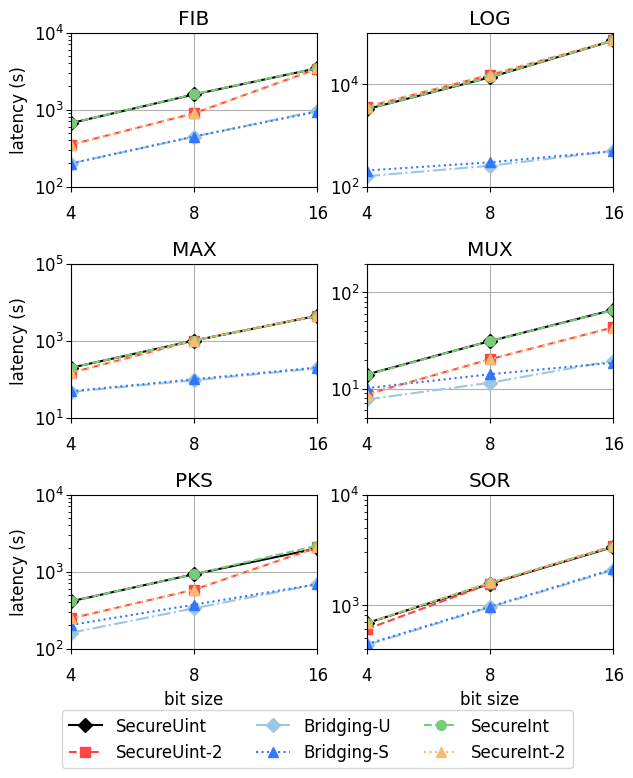
\includegraphics[width=\linewidth]{img/cases_latency.png}}
	\caption{Latency time for six benchmarks\iffalse using \secuint, \secint, unsigned and signed bridging, \texttt{Bridging-U} and \texttt{Bridging-S}, respectively,\fi with $t=2^{16}+1$. \iffalse In addition, we evaluate the benchmarks using \secuint\ and \secint\ with $t=2$ (postfix \texttt{-2}). \fi}
	\label{fig:benchmarks}
	\vspace{-0.4cm} 
\end{figure}

\innersection{Effect of plaintext modulus} Although $t=2$ does not enable batching in BFV, and therefore, it would not be used in practice, we compare it against the smallest plaintext modulus that enables batching ($t=2^{16}+1$) for $n=2^{15}$. The plaintext modulus does not affect the latency time to execute a homomorphic operation, but some homomorphic gates simplify in modulo 2 (e.g. XOR), as we discuss in Section \ref{ss:modcom}. Thus, a Boolean circuit used in bit-level arithmetic should have lower latency for $t=2$ if it contains XOR or XNOR gates. In Fig. \ref{fig:benchmarks}, we can see that in fact some applications are faster in modulo 2 (\texttt{SecureUint-2} and \texttt{SecureInt-2} for unsigned and signed bit-level arithmetic with $t=2$). MUX is the simplest benchmark, containing in bit-level arithmetic one equality, two \secbool-\secuint\ multiplications (or \secbool-\secint\ for signed numbers), one negation, and one addition. A \secbool-\secuint\ multiplication is entirely composed of XOR gates, and around half of the gates in the equality are XOR or XNOR. These operations are mainly responsible for the speed-up. 

% We have a similar situation for FIB and PKS, however here there are relatively fewer \secbool-\secuint\ multiplications and more additions, diminishing the effect of operating in modulo 2. The other benchmarks are much more complex applications and we noticed no difference in latency time between $t=2$ and $t=2^{16}+1$.

\innersection{Bit-level arithmetic vs bridging} Fig. \ref{fig:benchmarks} presents the latency time comparison between bit-level arithmetic and bridging. Regarding unsigned numbers (\secuint\ vs \texttt{Bridging-U}), results show that bridging outperforms bit-level arithmetic for all benchmarks and bit sizes. For some applications, like SOR, the performance improvement is limited (around 60\% speed-up). This happens because this algorithm requires many non-native operations (comparisons) in most stages. Only in the last part of the algorithm bridging can be employed, since using bridging before would require the inefficient conversion from \secmod\ to \secuint\ in order to execute the latter comparisons. Conversely, the logistic regression benefits a lot from using bridging with a speed-up of more than two orders of magnitude. This is possible because the non-native operations required by the filtering function are executed first. Therefore, at the filtering stage it is already possible to employ bridging and perform the remaining computation using the faster modular arithmetic.

\innersection{Signed numbers} Also in Fig. \ref{fig:benchmarks} we compare how bridging behaves with signed numbers. \iffalse In general, the extra conversion time required for signed numbers has little effect in the latency since the application uses significantly more multiplications compared to all the conversions. \fi We can see some degradation in PKS (4 bits) and MUX (4 and 8 bits). In PKS, there is conversion from \secint\ to \secmod\ in every iteration of the loop. The slowest operation in the loop is the comparison. This comparison operation is faster for smaller circuits (4 bits); therefore, the proportional latency of the two ciphertext multiplications required for the \secint\ to \secmod\ conversion is higher. For larger circuits, the comparison becomes more costly, thus, amortizing the conversion cost.

% Regarding MUX, it is a very simple function. It consists only of a comparison followed by a selection of one of two items. The explanation is similar to PKS, but the signed conversion has a higher impact in the latency time because there are two conversions instead of one in this algorithm.

\begin{figure}[t]
    % \vspace{-0.2cm}
	\centering
    \frame{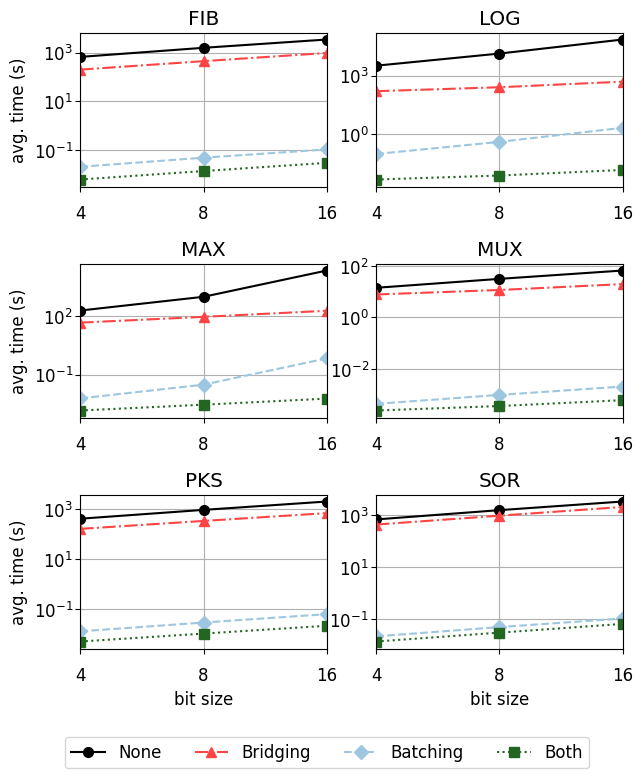
\includegraphics[width=\linewidth]{img/batching.png}}
	\caption{Average execution time for six benchmarks. \iffalse using and four cases: \texttt{None}: without bridging and batching, \texttt{Bridging}: with bridging only, \texttt{Batching}: with batching only, and \texttt{Both}: with both bridging and batching.\fi}
	\label{fig:batching}
	\vspace{-0.4cm} 
\end{figure}



\innersection{Bridging can be used with batching} Batching is a powerful technique used in FHE to pack many plaintexts into a ciphertext. The number of plaintexts that can be packed into a ciphertext is equal to the polynomial degree ($n = 2^{15}$ in our case). Although carefully crafted algorithms using batching and rotations can reduce program latency, the main benefit of batching is increased throughput, since it is possible to process $n$ plaintexts at once. Bridging on the other hand always reduces latency, and consequently improves throughput.
Bridging is a technique independent of batching and both can be used in tandem.
In Fig. \ref{fig:batching} we present the average execution time ($\text{latency} / \text{\# plaintexts packed}$) for six benchmarks and four cases: no batching and no bridging (\texttt{None}), bridging-only (\texttt{Bridging}), batching-only (\texttt{Batching}), and batching and bridging together (\texttt{Both}).
As expected, the throughput improvement provided by batching is impressive. However, for this technique to be used at its fullest, it is necessary to fill all ciphertext slots with plaintexts, which is the case with embarrassingly parallel workload. If the load is less than $n$, the performance will degrade.
Bridging does not suffer from this problem since it focuses on reducing the latency.
Nevertheless, bridging can be used in combination with batching. In this case, the speed-up of both techniques is added, leading to an even faster runtime (acceleration by more than 6 orders of magnitude (LOG)).

\innersection{Insights}
Bridging demonstrates substantial performance improvement for algorithms that allow mixing \secuint{} and \secmod{}, while in the worst case, bridging is equivalent to bit-level arithmetic. \iffalse This would happen if all outputs of a program come out from non-native operations. \fi
The comparison heavy SOR benefits less from bridging since these operations occur throughout the program and near the output, which precludes using the \secmod{} type in an earlier stage. On the contrary the benchmarks containing non-native operations near the beginning exhibit more significant performance improvements (MAX, FIB, PKS).
\iffalse At first glance, the MAX algorithm looks similar to SOR. However, some subtle differences in the \texttt{selection} function allow us to use bridging much earlier in the program; in fact, near the beginning of the application, leading to a much more noticeable performance improvement. 
FIB, and PKS have comparisons in all iterations, but since these comparisons are at the beginning of each iteration, bridging provides substantial performance improvements. \fi
Bridging benefits are maximized when non-native operations (e.g. comparisons) are at the beginning of the computation and the remaining of the computation can be done in modular arithmetic. The non-native operation would require the whole computation to work on bit-level arithmetic, but with bridging it becomes much faster since only the non-native operations are performed with \secuint, while the remaining run using \secmod. This is demonstrated by our logistic regression benchmark, which provides more than two orders of magnitude (precisely 143 times) of performance improvement.

% Finally, it is possible to combine bridging with batching for further performance improvement since both techniques are orthogonal to each other. It should be noted that this performance improvement is tightly connected to the parallelization capabilities of the workload. Nevertheless, results show that some benchmarks, when \emph{both} batching and bridging are combined, can be accelerated by more than 6 orders of magnitude (LOG).

\vspace{-0.1cm}
\section*{Resources}

Bridging has been integrated with the E3 framework and is available on github.com/momalab/e3 from commit \#88a323f.
\subsection{Discussion on practical use of bridging}\label{ss:discussion}

In Table \ref{tab:conversion}, we present the conversion cost from \secuint\ and \secint\ to \secmod, and vice-versa, considering several bit sizes ($s \in \{4, 7, 8, 16\}$) and plaintext moduli ($t \in \{2^4+1, 2^7+1, 2^{16}+1\}$)\review{, while Table \ref{tab:general} shows the general terms}.
Converting from \secuint\ to \secmod\ does not use ciphertext multiplications; therefore it is very efficient.
A conversion from \secint\ to \secmod\ needs only two multiplications, the cost of which is amortized since expensive bit-level arithmetic multiplications are avoided.

On the other hand, conversion from \secmod\ to \secuint\ is very costly.
A ciphertext multiplication in Microsoft SEAL BFV with polynomial degree $n = 2^{15}$ takes around 0.41s using the experimental setup described in Section \ref{ss:setup}, and the smallest plaintext modulus for $n = 2^{15}$ that enables batching is $t = 2^{16}+1$.
In this scenario, a conversion from \secmod\ to \secuint\ would take more than a week, while converting from \secmod\ to \secint\ takes nearly double that time.
Practical times for the conversion could be achieved only for very small plaintext moduli, in the order of $2^4+1$. Such small moduli is meaningful only with the BGV encryption scheme, which supports much smaller plaintext moduli with batching.
Considering comparable time for ciphertext multiplication, it would be possible to convert from \secmod\ to \secuint\ under one minute for 4 bits of precision ($s = 4$ and $t = 2^4+1$), and in around 12 minutes for 7 bits of precision ($s = 7$ and $t = 2^7+1$).


\vspace{-0.8cm}
\section*{Appendix}
\vspace{-0.2cm}
We include in this appendix the codes referent to the benchmarks used in \ref{ss:benchmarks}. The codes presented feature \secint, but the code using \secuint\ is similar.

\vspace{-0.1cm}
\begin{figure}[h]

%\scriptsize
% \vbox to 600pt {
\noindent\begin{minipage}{.50\textwidth}
\begin{lstlisting}[language=C++,
caption={Private Keyword Search using bit-level arithmetic.},
style=mystyle, label=list:pks_bit,
%framexrightmargin=-37pt,
% xleftmargin=0.4cm,
% xrightmargin=-0.12\linewidth,
% linewidth=0.88\linewidth
]
template <int S> SecureInt<S>
pks(vector<SecureInt<S>> v, SecureInt<S> k)
{
    vector<SecureInt<S>> r;
    for (size_t i=0; i < v.size(); i++)
    {
        auto eq = i == k;
        auto sel = eq * v[i];
        r.push_back(sel);
    }
    return sum(r);
}
\end{lstlisting}
\end{minipage}
% \vspace{\lstbspace}


% }
\end{figure}

\vspace{-1.3cm}
\begin{figure}[h]
%\scriptsize
\noindent\begin{minipage}{.50\textwidth}
\begin{lstlisting}[language=C++,
caption={Private Keyword Search with bridging.},
style=mystyle, label=list:pks_bridge,
%framexrightmargin=-37pt,
% xleftmargin=0.4cm,
% xrightmargin=-0.12\linewidth,
% linewidth=0.88\linewidth
]
template <int S> SecureMod
pks(vector<SecureInt<S>> v, SecureInt<S> k)
{
    vector<SecureMod> r;
    for (size_t i=0; i < v.size(); i++)
    {
        auto eq = i == k;
        auto sel = eq * SecureMod(v[i]);
        r.push_back(sel);
    }
    return sum(r);
}
\end{lstlisting}
\end{minipage}
% \vspace{\lstbspace}
\end{figure}


% \begin{figure}[t]
% %\scriptsize
% \noindent\begin{minipage}{.45\textwidth}
% \begin{lstlisting}[language=C++,
% caption={Private Keyword Search with bridging.},
% style=mystyle, label=list:pks_bit,
% %framexrightmargin=-37pt,
% % xleftmargin=0.4cm,
% % xrightmargin=-0.12\linewidth,
% % linewidth=0.88\linewidth
% ]
% template <int S> SecureMod
% pks(vector<SecureInt<S>> v, SecureInt<S> k)
% {
%     vector<SecureMod> r;
%     for (size_t i=0; i < v.size(); i++)
%     {
%         auto eq = i == k;
%         auto sel = eq * SecureMod(v[i]);
%         r.push_back(sel);
%     }
%     return sum(r);
% }
% \end{lstlisting}
% \end{minipage}
% % \vspace{\lstbspace}
% \end{figure}




\begin{figure}[t]
%\scriptsize
\begin{minipage}{\linewidth}
\begin{lstlisting}[language=C++,
caption={Logistic regression with data filtering using bit-level arithmetic.},
style=mystyle, label=list:log_bit,
%framexrightmargin=-37pt,
% xleftmargin=0.4cm,
% xrightmargin=-0.12\linewidth,
% linewidth=0.88\linewidth
]
template <class T> vector<vector<T>>
appendCol(vector<vector<T>> m, T value)
{
  for (auto & v : m) v.push_back(value);
  return m;
}

template <int S>
vector<vector<SecureInt<S>>>
filter(vector<vector<SecureInt<S>>> m,
  SecureInt<S> threshold, vector<int> pos)
{
  for (auto & idx : pos)
  {
    for (auto & v : m)
    {
      auto cond = v[idx] > threshold;
      v[idx] = cond * threshold
            + !cond * v[idx];
    }
  }
  return m;
}

template <int S>
vector<vector<SecureInt<S>>>
mm(vector<vector<SecureInt<S>>> a,
  vector<vector<SecureInt<S>>> b)
{
  auto n = a.size();
  auto m = b.size();
  auto p = b[0].size();
  vector<vector<SecureInt<S>>> c(n);
  for (size_t i=0; i<n; i++)
  {
    for (size_t j=0; j<p; j++)
    {
      vector<SecureInt<S>> t;
      for (size_t k=0; k<m; k++)
        t.push_back(a[i][k] * b[k][j]);
      c[i].push_back(sum(t));
    }
  }
  return c;
}

template <int S>
vector<vector<SecureInt<S>>>
logreg(vector<vector<SecureInt<S>>> inputs,
  vector<vector<SecureInt<S>>> weights,
  SecureInt<S> threshold, vector<int> pos)
{
  SecureInt<S> one = _1_E;
  filter(inputs, threshold, pos);
  auto inputsU = convert(inputs, one);
  appendCol(inputsU, one);
  return mm(inputsU, weights);
}
\end{lstlisting}
\end{minipage}
% \vspace{\lstbspace}
\end{figure}

\begin{figure}[b]
%\scriptsize
\begin{minipage}{\linewidth}
\begin{lstlisting}[language=C++,
caption={Logistic regression with data filtering using bridging.},
style=mystyle, label=list:log_bridge,
%framexrightmargin=-37pt,
% xleftmargin=0.4cm,
% xrightmargin=-0.12\linewidth,
% linewidth=0.88\linewidth
]
template <class T> vector<vector<T>>
appendCol(vector<vector<T>> m, T value)
{
  for (auto & v : m) v.push_back(value);
  return m;
}

template <int S>
vector<vector<SecureInt<S>>>
filter(vector<vector<SecureInt<S>>> m,
  SecureInt<S> threshold, vector<int> pos)
{
  for (auto & idx : pos)
  {
    for (auto & v : m)
    {
      auto cond = v[idx] > threshold;
      v[idx] = cond * threshold
            + !cond * v[idx];
    }
  }
  return m;
}


vector<vector<SecureMod>>
mm(vector<vector<SecureMod>> a,
  vector<vector<SecureMod>> b)
{
  auto n = a.size();
  auto m = b.size();
  auto p = b[0].size();
  vector<vector<SecureMod>> c(n);
  for (size_t i=0; i<n; i++)
  {
    for (size_t j=0; j<p; j++)
    {
      vector<SecureMod> t;
      for (size_t k=0; k<m; k++)
        t.push_back(a[i][k] * b[k][j]);
      c[i].push_back(sum(t));
    }
  }
  return c;
}

template <int S>
vector<vector<SecureMod>>
logreg(vector<vector<SecureInt<S>>> inputs,
  vector<vector<SecureMod>> weights,
  SecureInt<S> threshold, vector<int> pos)
{
  SecureMod one = _1_M;
  filter(inputs, threshold, pos);
  auto inputsU = convert(inputs, one);
  appendCol(inputsU, one);
  return mm(inputsU, weights);
}
\end{lstlisting}
\end{minipage}
% \vspace{\lstbspace}
\end{figure}


\begin{figure}[t]
%\scriptsize
\begin{minipage}{\linewidth}
\begin{lstlisting}[language=C++,
caption={Bit-level depth-optimized max function.},
style=mystyle, label=list:max_bit,
%framexrightmargin=-37pt,
% xleftmargin=0.4cm,
% xrightmargin=-0.12\linewidth,
% linewidth=0.88\linewidth
]









template <int S> vector<SecureInt<S>>
indices(vector<SecureInt<S>> v)
{
  int size = v.size();
  vector<SecureInt<S>> idx;
  vector<vector<SecureInt<S>>> m(size);
  for (int i=0; i < size; i++)
  {
    for (int j=i+1; j < size; j++)
    {
      auto cond = v[i] > v[j];
      m[i].push_back(SecureInt<S>(cond));
      m[j].push_back(SecureInt<S>(!cond));
    }
    idx.push_back(product(m[i]));
  }
  return idx;
}

template <int S> SecureInt<S>
select(vector<SecureInt<S>> idx,
  vector<SecureInt<S>> v)
{
  int size = v.size();
  vector<SecureInt<S>> r;
  for (int i=0; i < size; i++)
    r.push_back(idx[i] * v[i]);
  return sum(r);
}

template <int S> SecureInt<S>
max(vector<SecureInt<S>> v)
{
  return select(indices(v), v);
}

\end{lstlisting}
\end{minipage}
% \vspace{\lstbspace}
\end{figure}

\begin{figure}[t]
%\scriptsize
\begin{minipage}{\linewidth}
\begin{lstlisting}[language=C++,
caption={The multiplexer function using bit-level arithmetic.},
style=mystyle, label=list:mux_bit,
%framexrightmargin=-37pt,
% xleftmargin=0.4cm,
% xrightmargin=-0.12\linewidth,
% linewidth=0.88\linewidth
]
template <int S> SecureInt<S>
mux(SecureInt<S> input, SecureInt<S> item,
    SecureInt<S> t, SecureInt<S> f)
{
    auto cond = input == item;
    return cond * t
        + !cond * f;
}
\end{lstlisting}
\end{minipage}
% \vspace{\lstbspace}
\end{figure}

\begin{figure}[t]
%\scriptsize
\begin{minipage}{\linewidth}
\begin{lstlisting}[language=C++,
caption={Depth optimized max function with bridging.},
style=mystyle, label=list:max_bridge,
%framexrightmargin=-37pt,
% xleftmargin=0.4cm,
% xrightmargin=-0.12\linewidth,
% linewidth=0.88\linewidth
]
template <class T> vector<SecureMod>
convert(vector<T> v)
{
    vector<SecureMod> u;
    for (auto & e : v)
        u.push_back(SecureMod(e));
    return u;
}

template <int S> vector<SecureMod>
indices(vector<SecureInt<S>> v)
{
  int size = v.size();
  vector<SecureMod> idx;
  vector<vector<SecureMod>> m(size);
  for (int i=0; i < size; i++)
  {
    for (int j=i+1; j < size; j++)
    {
      auto cond = v[i] > v[j];
      m[i].push_back(SecureMod(cond));
      m[j].push_back(SecureMod(!cond));
    }
    idx.push_back(product(m[i]));
  }
  return idx;
}

SecureMod
select(vector<SecureMod> idx,
    vector<SecureMod> v)
{
  int size = v.size();
  vector<SecureMod> r;
  for (int i=0; i < size; i++)
    r.push_back(idx[i] * v[i]);
  return sum(r);
}

template <int S> SecureMod
max(vector<SecureInt<S>> v)
{
  return select(indices(v), convert(v));
}
\end{lstlisting}
\end{minipage}
% \vspace{\lstbspace}
\end{figure}

\begin{figure}[t]
%\scriptsize
\begin{minipage}{\linewidth}
\begin{lstlisting}[language=C++,
caption={The multiplexer function with bridging.},
style=mystyle, label=list:mux_bridge,
%framexrightmargin=-37pt,
% xleftmargin=0.4cm,
% xrightmargin=-0.12\linewidth,
% linewidth=0.88\linewidth
]
template <int S> SecureMod
mux(SecureInt<S> input, SecureInt<S> item,
    SecureInt<S> t, SecureInt<S> f)
{
    auto cond = input == item;
    return cond * SecureMod(t)
        + !cond * SecureMod(f);
}
\end{lstlisting}
\end{minipage}
% \vspace{\lstbspace}
\end{figure}


\begin{figure}[t]
%\scriptsize
\begin{minipage}{\linewidth}
\begin{lstlisting}[language=C++,
caption={Depth-optimized sorting algorithm using bit-level arithmetic.},
style=mystyle, label=list:sor_bit,
%framexrightmargin=-37pt,
% xleftmargin=0.4cm,
% xrightmargin=-0.12\linewidth,
% linewidth=0.88\linewidth
]









template <int S> vector<SecureInt<S>>
indices(vector<SecureInt<S>> v)
{
  int size = v.size();
  vector<SecureInt<S>> idx;
  vector<vector<SecureInt<S>>> m(size);
  for (int i=0; i < size; i++)
  {
    for (int j=i+1; j < size; j++)
    {
      auto cond = v[i] > v[j];
      m[i].push_back(SecureInt<S>(cond));
      m[j].push_back(SecureInt<S>(!cond));
    }
    idx.push_back(sum(m[i]));
  }
  return idx;
}

template <int S> vector<SecureInt<S>>
select(vector<SecureInt<S>> idx,
  vector<SecureInt<S>> v)
{
  int size = v.size();
  vector<SecureInt<S>> r;
  for (int i=0; i < size; i++)
  {
    vector<SecureInt<S>> t;
    for (int j=0; j < size; j++ )
      t.push_back((i == idx[j]) * v[j]);
    r.push_back(sum(t));
  }
  return r;
}

template <int S> vector<SecureInt<S>>
sort(vector<SecureInt<S>> v)
{
  return select(indices(v), v);
}

\end{lstlisting}
\end{minipage}
% \vspace{\lstbspace}
\end{figure}

\begin{figure}[t]
%\scriptsize
\begin{minipage}{\linewidth}
\begin{lstlisting}[language=C++,
caption={Depth-optimized sorting algorithm using bridging.},
style=mystyle, label=list:sor_bridge,
%framexrightmargin=-37pt,
% xleftmargin=0.4cm,
% xrightmargin=-0.12\linewidth,
% linewidth=0.88\linewidth
]
template <class T> vector<SecureMod>
convert(vector<T> v)
{
    vector<SecureMod> u;
    for (auto & e : v)
        u.push_back(SecureMod(e));
    return u;
}

template <int S> vector<SecureInt<S>>
indices(vector<SecureInt<S>> v)
{
  int size = v.size();
  vector<SecureInt<S>> idx;
  vector<vector<SecureInt<S>>> m(size);
  for (int i=0; i < size; i++)
  {
    for (int j=i+1; j < size; j++)
    {
      auto cond = v[i] > v[j];
      m[i].push_back(SecureInt<S>(cond));
      m[j].push_back(SecureInt<S>(!cond));
    }
    idx.push_back(sum(m[i]));
  }
  return idx;
}

template <int S> vector<SecureMod>
select(vector<SecureInt<S>> idx,
  vector<SecureMod> v)
{
  int size = v.size();
  vector<SecureMod> r;
  for (int i=0; i < size; i++)
  {
    vector<SecureMod> t;
    for (int j=0; j < size; j++ )
      t.push_back((i == idx[j]) * v[j]);
    r.push_back(sum(t));
  }
  return r;
}

template <int S> vector<SecureMod>
sort(vector<SecureInt<S>> & v)
{
  return select(indices(v), convert(v));
}


\end{lstlisting}
\end{minipage}
% \vspace{\lstbspace}
\end{figure}


\subsection{Modular and bit-level arithmetic}\label{ss:modcom}

Some FHE schemes define arithmetic addition, subtraction, and multiplication on numeric rings, but not other arithmetic such as division or comparison. While some applications may not require any other operation, a programmer is accustomed to having all programming operations available in their programs.
For example, the C++ statement "{\tt{}if(a<b)c+=a}" and its corresponding data-oblivious form: "{\tt{}c+=(a<b)*a}", cannot be evaluated with an FHE scheme where the comparison operation is not defined.
Notably, addition, subtraction, and multiplication on integers is an incomplete set of arithmetic operations; for instance, the comparison operation cannot be reduced to these three operations. However, when operating on bits, the same set of operations is universal, having addition and subtraction correspond to logical \texttt{XOR} and multiplication to logical \texttt{AND}.

\eee\ solves this problem by allowing the programmer to use data types constructed out of sequences of encrypted bits. Indeed, as the least possible requirement to the computing capacity, an FHE scheme must be able to evaluate the logic \texttt{NAND} (or \texttt{NOR}) gate on ciphertexts, since this elementary function is sufficient for universal computation. 
In this way, the variables in the expression "{\tt{}c+=(a<b)*a}" are defined as \emph{integral types} where all three operations (comparison, multiplication, and addition) are performed using bit-level arithmetic circuits. We call this computation {\it bit-level arithmetic}, as opposed to the natively provided {\it modular arithmetic}, where addition and multiplication are performed directly on ciphertexts.

The transition from modular to bit-level arithmetic is straightforward: Since
the encrypted bit values are limited to 0 and~1, logic gates, such as \texttt{AND}, \texttt{XOR}, \texttt{NOT}, etc, can be expressed via the following expressions:
\vspace{-0.2cm}
\begin{equation*}\label{eq:logic}
\begin{split}
x \ \texttt{AND} \ y = xy,& \qquad x \ \texttt{NAND} \ y = 1-xy \\
x \ \texttt{OR} \ y = x+y-xy,& \qquad x \ \texttt{NOR} \ y = 1-(x \ \texttt{OR} \ y) \\
x \ \texttt{XOR} \ y = x+y-2xy,& \qquad x \ \texttt{XNOR} \ y = 1-(x \ \texttt{XOR} \ y) \\
 \texttt{NOT} \ x = 1-x,& \qquad \texttt{MUX}(x,y,z) = x(y-z)+z, \\
\end{split}
\end{equation*}

\noindent where \texttt{MUX} is the multiplexer operation (as in {$x$?$y$:$z$}). The set of values $\{0,1\}$ is closed under the above set of expressions. 
In this paper, we use the term \emph{homomorphic gates} to describe logic gates operating on encrypted bits. Given these homomorphic gates, higher level operations (comparison, addition, multiplication) can be built using standard combinational arithmetic circuit design, which allows to perform any programming operation, i.e. giving the full spectrum of C++ arithmetic. Gate equations simplify for plaintext modulo $2$; e.g. XOR gate does not require multiplication, as \mbox{$x \ \texttt{XOR} \ y = x+y \bmod 2$}.

\innersection{Data types}
We define three data types for bit-level arithmetic, \secuint, \secint, and \secbool, and one for modular arithmetic, \secmod. 
A \secuint\ or \secint\ variable is an array of ciphertexts, each encrypting either zero or one. \secuint\ is comparable to \texttt{unsigned int}, while \secint\ corresponds to \texttt{int}.
The third type is \secbool, which is a type derived from \secuint\texttt{<1>}. It is the secure equivalent of \texttt{bool}.
For modular arithmetic, there is only the native type, which operates modulo the plaintext modulus. We call this type \secmod.

With bit-level arithmetic, we can express programs with operations not supported by modular arithmetic.
Listing~\ref{list:fibs} demonstrates the transition from plaintext computation to secure computation: Integer variables are declared with the secure type \secuint; the rest of the code remains the same.
%\footnote{\secuint\ is the secure equivalent of \texttt{unsigned int}. We discuss signed integers later.} Note that the type is parameterized with the size. 
In encrypted computation, increasing the number of bits of integral types can lead to a dramatic increase in performance overhead.
For this reason, we define the bit size as a template specialization.
% As experimental results demonstrate, even 1 bit can make significant difference in performance, affecting the practicality dimension. 
Explicit size declaration can be found in functional programming languages, so the programmer may already be familiar with this practice.
In the example of Listing~\ref{list:fibs}, all variables are 8 bits (lines 3, 4).

The postfix {\tt{}\_E} after each constant provides encrypted values used in variable initialization of integral type variables.
% The configuration file with the specifications of the encryption defines the type name and postfix used for constants in the program.
\eee\ automatically encrypts and replaces the plaintext constants with their encrypted representations, so the final binary does not have information about the initial values used in the program. 

\begin{figure}
%\scriptsize
\begin{minipage}{\linewidth}
\begin{lstlisting}[language=C++, caption={Secure version of Fibonacci function. Type \secuint\ behaves as native {\tt unsigned int}.
% \hspace{-1.40cm} \mbox{}
}, style=mystyle, label=list:fibs,
% xrightmargin=-0.12\linewidth,
% linewidth=0.96\linewidth
]
SecureUint<8> fibonacci(SecureUint<8> in)
{
    SecureUint<8> i=_0_E, a=_0_E, b=_1_E;
    SecureUint<8> r=_0_E;
    int max_iter = 10;
    while( max_iter-- )
    {
        r += (i++ == in) * a;
        std::swap(a,b);
        a += b;
    }
    return r;
}
\end{lstlisting}

\vspace{-0.5cm} 

% \vspace{0.2in}

% \begin{lstlisting}[language=C++, caption={An outline example of \secint\ definition.
% % \hspace{-1.40cm} \mbox{}
% }, style=mystyle, label=list:ciro,
% % xrightmargin=-0.12\linewidth,
% % linewidth=0.96\linewidth
% ]
% template <int Size> class SecureUint{ ... };
% constexpr std::string operator""_E
%   (unsigned long long int x){ ... }
% \end{lstlisting}
\end{minipage}
% \vspace{\lstbspace}
% \vspace{-0.8cm}
\end{figure}



\subsection{Bridging modular and bit-level arithmetic}\label{ss:bridging}

Declaring variables with a protected integral type and using solely bit-level arithmetic as in Listing~\ref{list:fibs} has a potential drawback: When an FHE scheme provides fast modular arithmetic operations, the usage of circuits operating on separate bits is slow. This paper brings the  idea of 
\textit{Bridging} - mixing both modular and bit-level arithmetic in one program with the ability to convert variables from one type to the other. %integral type to modular.
Some variables can be declared using a protected type supporting only modular arithmetic, while others with another secure type supporting bit-level arithmetic. In bridging mode, a type of bit-level arithmetic declares a conversion function into a type of modular arithmetic, and vice-versa.
In all cases, the encryption of the two different C++ types must share the same FHE keys, which is ensured by our proposed methodology and framework. 

\subsubsection{\secuint\ to \secmod{}}\label{sss:secuint2secmod}

For performance reasons, it is desirable to execute the entire computation in modular arithmetic, since it is much faster than bit-level. If however, a program requires an operation not supported in modular arithmetic (e.g., comparison), then, without Bridging, the whole program must perform all computations using bit-level arithmetic, severely degrading performance. 
In effect, Bridging enables the isolation of the parts of the computation requiring bit-level arithmetic.
For example, the expression "{\tt{}c+=(a<b)*a}" can use bit-level arithmetic for the comparison only.
The variables required by the comparison (i.e., \texttt{a} and \texttt{b}) must be of integral type. Nevertheless, the operands of the multiplication can be cast to our modular type, allowing multiplication and addition to be executed in modular arithmetic, resulting in a variable {\tt{}c} of modular type.

\begin{figure}
%\scriptsize
\begin{minipage}{\linewidth}
\begin{lstlisting}[language=C++, caption={
Bridging (i.e.,~mixing \secmod{} and \secuint\ types) enables performance improvement. The postfix \texttt{\_M} denotes encrypted variable for the \secmod\ type.
},
style=mystyle, 
label=list:fibm,
xleftmargin=0.45cm,
% xrightmargin=-0.12\linewidth,
% linewidth=0.88\linewidth
]
SecureMod fibonacci(SecureUint<8> in)
{
    SecureUint<8> i=_0_E;
    SecureMod a=_0_M, b=_1_M, r=_0_M;
    int max_iter = 10;
    while( max_iter-- )
    {
        r += (i++ == in) * a;
        std::swap(a,b);
        a += b;
    }
    return r;
}
\end{lstlisting}
\end{minipage}
% \vspace{\lstbspace}
\vspace{-0.8cm}

\end{figure}
% \vspace{-1cm} 

Listing~\ref{list:fibm} demonstrates the code of the Fibonacci function of Listing~\ref{list:fibs} with \emph{Bridged} arithmetic: Only the input \texttt{in} and counter \texttt{i} are declared as integral type \secuint{}, while the others are replaced with the faster \secmod\ type. 
Line 8 does implicit conversion from \secuint\ to \secmod;
in this way, bit-level multiplication (which is slow) is not executed. Instead, only the native (much faster) multiplication of ciphertexts is needed.
Specifically, the comparison between {\tt i} and {\tt in} is the slowest operation in the program, and its result is one encrypted bit which can naturally be casted to \secmod, since the set $\{0,1\}$ is a subset of the plaintext range.
The operation for casting an integral type (bit-level) into modular (FHE native) is a summation of the encrypted bits of the integral type. 
In fact, the binary representation of a value $X$ can be reorganized by {\it Horner's scheme} in a set of additions over its $s$ bits $x_i$:
\begin{equation*}
\begin{split}
X & = 2^{s-1}x_{s-1} +2^{s-2}x_{s-2} + ... + 2x_1+x_0 = \\
& =(...((x_{s-1})\cdot 2+x_{s-2})\cdot 2+...+x_1)\cdot 2+x_0
\end{split}
\end{equation*}

Evaluating the right hand side of the above equation yields the value corresponding to the bit sequence. This evaluation is an efficient way to convert a program variable of type \secuint{} into a \secmod{} value.
Listing~\ref{list:secuint2secmod} shows the C++ implementation of such casting.
We emphasize that this conversion requires no ciphertext multiplications, only additions. Specifically, $2 \cdot (s - 1)$ ciphertext additions with a maximum additive depth of $s-1$, where $s$ is the number of encrypted bits.

\begin{figure}[t]
%\scriptsize
\begin{minipage}{\linewidth}
\begin{lstlisting}[language=C++, caption={
Casting from \secuint\ to \secmod. Since the former is a set of ciphertexts representing encrypted bits, it is possible to access each bit individually.}, style=mystyleb, label=list:secuint2secmod,
%framexrightmargin=-37pt,
% xleftmargin=0.4cm,
% xrightmargin=-0.12\linewidth,
% linewidth=0.88\linewidth
]
template <int Size>
SecureMod to_SecureMod(SecureUint<Size> v)
{
    auto i = Size;
    SecureMod r = v[--i];
    while ( i-- ) r += r + v[i];
    return r;
}
\end{lstlisting}
\end{minipage}
% \vspace{\lstbspace}
\vspace{-0.5cm} 
\end{figure}

\begin{figure}[t]
%\scriptsize
\begin{minipage}{\linewidth}
\begin{lstlisting}[language=C++, caption={
Casting from \secint\ to \secmod. The \secint\ variable is converted to \secuint, which is then converted to \secmod.}, style=mystyleb, label=list:secint2secmod,
%framexrightmargin=-37pt,
% xleftmargin=0.4cm,
% xrightmargin=-0.12\linewidth,
% linewidth=0.88\linewidth
]
template <int Size>
SecureMod to_SecureMod(SecureInt<Size> v)
{
    SecureUint<Size> u(v);
    auto pos = to_SecureMod(u);
    int max = 1 << Size;
    auto neg = SecureMod::t - max + pos;
    SecureMod isNeg = v[Size-1];
    return isNeg * neg + (1-isNeg) * pos;
}
\end{lstlisting}
\end{minipage}
% \vspace{\lstbspace}
\vspace{-0.7cm} 
\end{figure}


% \iffalse Then, we use the most significant bit of the \secint\ variable to define whether the value is negative. \if 

Line 8 of Listing~\ref{list:fibm} does implicit conversion of \secbool{} to \secmod{}. Note that \secbool\ is a derived class from \secuint\texttt{<1>}. To observe a more complex scenario, consider the expression "{\tt{}c+=(a==b)*a}" that actually requires conversion of \secuint{}.
Comparison between \texttt{a} and \texttt{b} must be evaluated in bit-level. This implies that types of \texttt{a} and \texttt{b} must be \secuint{}. The comparison is done on a bit-by-bit manner using homomorphic gates following the gate equations described in Section \ref{ss:modcom}.
The gates correspond to normal logic gates, but operating on ciphertexts instead of ordinary bits. The result of the comparison is one encrypted bit represented by type \secbool.
Multiplication between a \secbool\ and a \secuint\ is evaluated as a multiplexer operation with $s$ \texttt{AND} gates, where $s$ is the number of encrypted bits in the \secuint\ variable, resulting in a \secuint{} type.
The type of variable \texttt{c} can be chosen as \secmod{}. The addition in the expression is then performed on variables of \secmod{} and \secuint{} types: "{\tt{}c=c+t}", where "{\tt{}t=(a==b)*a}". Implicit conversion evokes our function of Listing \ref{list:secuint2secmod} from the constructor of \secmod{} type out of \secuint{}.
Then the addition operation follows on two variables, both of the \secmod{} type.

It should be noted that all these conversions and evaluations are done obliviously to the user and do not require special attention; the user writes only "{\tt{}c+=(a==b)*a}".
A more efficient way to perform this computation is to explicitly convert argument \texttt{a}  in this expression to \secmod. In such case, the multiplication is done in modular arithmetic which is around $s$ times faster than a multiplication between \secbool{} and \secuint{} (and many more times faster than multiplying two \secuint{}s).\footnote{The exact speed-up compared to multiplying two \secuint s depends on the variables' bit size.} The corresponding expression becomes \mbox{"{\tt{}c+=(a==b)*\secmod(a)}"}.
Same way as above, the constructor calls the conversion function (Listing~\ref{list:secuint2secmod}), this time one step earlier - before the multiplication - resulting in having a larger portion of the computation in modular arithmetic, hence improving the performance.
It it worth noting that while there is automatic conversion from \secuint\ to \secmod, it is the programmer's task to define each variable's type and, in some cases, call conversion explicitly for better performance.

\subsubsection{\secint\ to \secmod{}}\label{sss:secint2secmod}

So far, we have discussed unsigned numbers. However, bit-level arithmetic also supports signed numbers following the two's complement arithmetic.
On the other hand, modular arithmetic only supports numbers in $\mathbb{Z}_t$, where $t$ is the plaintext modulus.
Nevertheless, it is possible to emulate negative numbers in modular arithmetic in the programmer's domain as in Cryptoleq \cite{cryptoleq}, where lower values are considered positive and large values are interpreted as negative numbers.
In this case, the conversion from a signed bit-level arithmetic type \secint\ to \secmod\ is defined as:
\begin{equation}
  X=\begin{cases}
    t - 2^s + \sum_{i=0}^{s-1}{(2^i \cdot x_i)}, & \text{if $x<0$}.\\
    \sum_{i=0}^{s-1}{(2^i \cdot x_i)}, & \text{otherwise}.
  \end{cases}
\end{equation}
where $s$ is the number of bits and $x_i$ is the bit of $x$ at position $i$. The condition $x < 0$ is determined by the most significant bit of $x$; thus, we can use it as a multiplexer between the two cases.
Listing \ref{list:secint2secmod} presents the algorithm for converting a \secint\ into a \secmod. First, the \secint\ is interpreted as a \secuint\ (line 4). In line 5, this value is converted into a \secmod\ using the algorithm of Listing \ref{list:secuint2secmod}.
Then in line 7, we perform the subtraction of plaintexts $t$ and \texttt{max} (i.e. $2^s$), and then do a ciphertext addition with the \secmod\ variable \texttt{pos}. At this point, we have generated two \secmod\ variables: \texttt{pos}, representing the value in case it is positive, and \texttt{neg} containing the value in case it is a negative number. This totals $2s - 1$ ciphertext additions with a additive depth of $s$.
Finally, we select between \texttt{neg} and \texttt{pos} using the most significant bit of the \secint\ input (lines 8-9). If the bit is one, it means it is a negative number; thus, we select \texttt{neg}; otherwise, we select \texttt{pos}.
For selection we need ciphertext multiplications.
The entire conversion from \secint\ to \secmod\ requires two ciphertext multiplications and $2s + 1$ ciphertext additions with a multiplicative depth equal to one.
By comparing Listings \ref{list:secuint2secmod} and \ref{list:secint2secmod}, we can see that converting signed numbers to \secmod\ is less efficient than converting unsigned numbers to \secmod. Furthermore, $t$ must be large enough ($t \geq 2^s$) to accommodate the converted value.

% \innersection{Why not signed and unsigned \secmod{}} \secmod{} types can only participate in addition, subtraction, and multiplication operations. The values of this type are elements of the corresponding mathematical ring. The programmer can choose to interpret a subset of the number space as negative, but there would be no difference in these computations. For this reason, there is no differentiation between the signed and unsigned versions for \secmod{} type.
\subsubsection{\secmod\ to \secuint{}}\label{sss:secmod2secuint}
\vspace{-0.2cm}
Conversion from \secmod\ to \secuint\ is theoretically possible using the expression:
\vspace{-0.2cm}
\begin{equation}\label{eq:secmod2secuint}
    \vspace{-0.1cm}
    X = \sum_{i=1}^{t-1}(i \cdot \secbool(1 - (x-i)^{t-1}))
\end{equation}
where $x$ is the \secmod\ variable to be converted, $t$ is the plaintext modulus and is prime, $i$ is a \secuint\ counter, and $X$ is the resulting \secuint. Due to the properties of modular arithmetic and the parameters used in homomorphic encryption, the exponentiation to $t-1$ results in zero in case the base is zero, and one otherwise. When $i = x$, the expression in the summation results in $i$, while in all other cases it will result in zero, since $1 - (x-i)^{t-1} = 0 \ \forall \ i \ne x$.
% Breaking down Eq. \ref{eq:secmod2secuint}:
% \begin{enumerate}
%     \item The \secuint\ $i$ is automatically cast to \secmod\ in $x-i$ before the exponentiation, resulting in a subtraction between two \secmod{}s.
%     \item The exponentiation of the \secmod\ $x-i$ to the integer $t-1$ results in a \secmod\ variable containing either the encryption of zero or one.
%     \item The result of the exponentiation is negated by subtracting it from one. At this point, we have the encryption of one in case $x = i$ and zero otherwise stored in a \secmod\ variable. In order to avoid automatically casting $i$ to \secmod\ in the multiplication, we must first reinterpret the partial result as \secbool.
%     \item We multiply the \secuint\ $i$ by the \secbool\ value resulting in a \secuint\ equal to $i$ or zero. We remark that a \secbool-\secuint\ multiplication is evaluated as a multiplexer operation.
%     \item We repeat this process for all $i \in [1,t)$, adding the resulting values. The final result is a \secuint\ equal to $x$ since there is only one $i$ that is equal to $x$.
% \end{enumerate}

An implementation of the fast exponentiation algorithm is presented in Listing \ref{list:pow}. The number of multiplications is given by $\floor{\log_2{e}} + \omega(e) - 1$ and the multiplicative depth is $\ceil{\log_2{e}}$, where $e$ is the exponent and $\omega(\cdot)$ is a function that calculates the Hamming weight. The conversion from \secmod\ to \secuint\ can exploit this property of the exponentiation to $t-1$ resulting in zero or one to create an equality function, where the equality function is given by $1 - (x-i)^{t-1}$. With this information, we can build a linear search to find the \secuint\ $i$ that is equal to the \secmod\ $x$ using the result of the equality as a selector. Listing \ref{list:secmod2secuint} presents the algorithm that performs this conversion.
The number of multiplications is given by $t \cdot (s + \floor{\log_2{(t-1)}} + \omega(t-1) - 1)$, while the multiplicative depth is equal to $\ceil{\log_2{(t-1)}} + 1$.
One can notice that this algorithm is only practical for small plaintext moduli $t$. Once $t$ becomes large, the linear search makes it impractical. Since \secmod\ requires a large $t$ for it to be useful, this conversion should not be used in practice and should be avoided, as later presented and discussed in Section~\ref{ss:conversion}.

\begin{figure}[t]
%\scriptsize
\begin{minipage}{\linewidth}
\begin{lstlisting}[language=C++, caption={
Homomorphic exponentiation function.}, style=mystyleb, label=list:pow,
%framexrightmargin=-37pt,
% xleftmargin=0.4cm,
% xrightmargin=-0.12\linewidth,
% linewidth=0.88\linewidth
]
SecureMod pow(SecureMod b, int e)
{
    if (e == 0) return SecureMod(1);
    if (e == 1) return b;
    auto r = pow(b * b, e >> 1);
    if (e & 1) r *= b;
    return r;
}
\end{lstlisting}
\end{minipage}
% \vspace{\lstbspace}
\vspace{-0.5cm} 
\end{figure}

\begin{figure}[!t]
%\scriptsize
\begin{minipage}{\linewidth}
\begin{lstlisting}[language=C++, caption={
Casting from \secmod\ to \secuint.}, style=mystyleb, label=list:secmod2secuint,
%framexrightmargin=-37pt,
% xleftmargin=0.4cm,
% xrightmargin=-0.12\linewidth,
% linewidth=0.88\linewidth
]
template <int Size>
SecureUint to_SecureUint<Size>(SecureMod x)
{
SecureMod one(1);
    auto & t = SecureMod::t;
    vector<SecureUint<Size>> v;
    for (int i = 1; i < t; i++)
    {
        auto si = SecureUint<Size>(i);
        auto eq = one - pow(x-i, t-1);
        v.push_back(si * SecureBool(eq));
    }
    return sum(v);
}
\end{lstlisting}
\end{minipage}
% \vspace{\lstbspace}
\vspace{-0.5cm} 
\end{figure}

% \begin{table*}[!th]
\centering
\begin{tabular}{cc|ccc|ccc|cc|cc}
  &   & \multicolumn{3}{c|}{\secuint\ \texttt{to} } & \multicolumn{3}{c|}{\secint\ \texttt{to} } & \multicolumn{2}{c|}{\secmod\ \texttt{to} } & \multicolumn{2}{l}{\secmod\ \texttt{to} } \\ 
  \multicolumn{1}{c}{} & \multicolumn{1}{c|}{} & \multicolumn{3}{c|}{\secmod{}}        & \multicolumn{3}{c|}{\secmod{}}      & \multicolumn{2}{c|}{\secuint{}}     & \multicolumn{2}{c}{\secint{}}     \\ \hline
s  & t & mul     & add     & depth    & mul     & add    & depth    & mul            & depth         & mul           & depth        \\ \hline
\normalfont{4}  & \unboldmath \( 2^{4} +1 \)  & \normalfont{0}         & \normalfont{6}         & \normalfont{0}       & \normalfont{2}         & \normalfont{9}        & \normalfont{1}       & \normalfont{136}              & \normalfont{5}            & \normalfont{274}             & \normalfont{6}           \\ \hline
\normalfont{7}  & \unboldmath \( 2^{7} +1 \)  & \normalfont{0}         & \normalfont{12}        & \normalfont{0}       & \normalfont{2}         & \normalfont{15}       & \normalfont{1}       & \normalfont{1778}             & \normalfont{8}            & \normalfont{3558}            & \normalfont{9}           \\ \hline
\normalfont{8}  & \unboldmath \( 2^{16} +1 \)  & \normalfont{0}         & \normalfont{14}        & \normalfont{0}       & \normalfont{2}         & \normalfont{17}       & \normalfont{1}       & \normalfont{1572888}          & \normalfont{17}           & \normalfont{3145778}         & \normalfont{18}          \\ \hline
\normalfont{16} & \unboldmath \( 2^{16} +1 \)  & \normalfont{0}         & \normalfont{30}        & \normalfont{0}       & \normalfont{2}         & \normalfont{33}       & \normalfont{1}       & \normalfont{2097184}          & \normalfont{17}           & \normalfont{4194370}         & \normalfont{18}         \\
\end{tabular}
\caption{Number of ciphertext additions and multiplications, and multiplicative depth for converting from \secuint\ and \secint\ to \secmod, and vice-versa. The results show that \secmod{} to \secuint\ and \secint\ conversion is impractical. The overhead from ciphertext additions for converting from \secmod\ to \secuint\ and \secint\ is negligible and not included.}
\label{tab:conversion}
\end{table*}



% \begin{table}[t]
    \centering
    \begin{tabular}{c|c|c}
         \review{\secuint{}}                & \review{mul}   & \review{\normalfont{0}}                                                           \\
         \review{\normalfont{to}}           & \review{add}   & \review{\normalfont{$2 \cdot (s - 1)$}}                                           \\
         \review{\secmod{}}                 & \review{depth} & \review{\normalfont{0}}                                                           \\ \hline
         \review{\secint{}}                 & \review{mul}   & \review{\normalfont{2}}                                                           \\
         \review{\normalfont{to}}           & \review{add}   & \review{\normalfont{$2s + 1$}}                                                    \\
         \review{\secmod{}}                 & \review{depth} & \review{\normalfont{1}}                                                           \\ \hline
         \review{\secmod{} \normalfont{to}} & \review{mul}   & \review{\tiny{$t \cdot (s + \floor{\log_2{(t-1)}} + \omega(t-1) - 1)$}}           \\
         \review{\secuint{}}                & \review{depth} & \review{\scriptsize{$\ceil{\log_2{(t-1)}} + 1$}}                                  \\ \hline
         \review{\secmod{} \normalfont{to}} & \review{mul}   & \review{\tiny{$2 \cdot t \cdot (s + \floor{\log_2{(t-1)}} + \omega(t-1) - 1)+2$}} \\
         \review{\secint{}}                 & \review{depth} & \review{\scriptsize{$\ceil{\log_2{(t-1)}} + 2$}}                                  \\
    \end{tabular}
    \caption{\review{General terms for the number of multiplications (mul), number of additions (add), and multiplicative depth (depth) for converting from \secuint\ and \secint\ to \secmod\ and vice-versa, where $s$ is the number of encrypted bits in the \secuint/\secint\ variable, $t$ is the plaintext modulus, and $\omega(\cdot)$ is the Hamming weight.}}
    \label{tab:general}
\end{table}


\subsubsection{\secmod\ to \secint{}}\label{sss:secmod2secint}

Conversion from \secmod\ to \secint\ is possible by applying Eq. \ref{eq:secmod2secint} to the result of Eq. \ref{eq:secmod2secuint}:
\begin{equation}\label{eq:secmod2secint}
    Y = (1 - X_{s-1}) \cdot X + X_{s-1} \cdot (2^s - t + X)
\end{equation}
$X$ is the result of Eq. \ref{eq:secmod2secuint}, $Y$ is the \secint\ output, $s$ is the number of encrypted bits in $X$ and $Y$, $t$ is the plaintext modulus, and $2^s \geq t$.
Listing \ref{list:secmod2secint} shows the algorithm for this conversion. It leverages the conversion described in Listing \ref{list:secmod2secuint} and adjusts for the sign.
This algorithm requires $2 \cdot t \cdot (s + \floor{\log_2{(t-1)}} + \omega(t-1) - 1)+2$ multiplications with a multiplicative depth of $\ceil{\log_2{(t-1)}} + 2$.

\begin{figure}[!t]
%\scriptsize
\begin{minipage}{\linewidth}
\begin{lstlisting}[language=C++, caption={
Casting from \secmod\ to \secint.}, style=mystyleb, label=list:secmod2secint,
%framexrightmargin=-37pt,
% xleftmargin=0.4cm,
% xrightmargin=-0.12\linewidth,
% linewidth=0.88\linewidth
]
template <int Size>
SecureInt to_SecureInt<Size>(SecureMod x)
{
    auto u = to_SecureUint<Size>(x);
    SecureInt<Size> pos(u);
    auto max = 1 << s;
    auto diff = max - SecureMod::t;
    u = to_SecureUint<Size>(diff + x);
    SecureInt<Size> neg(u);
    auto & isNeg = pos[s-1];
    return isNeg * neg + (1-isNeg) * pos;
}
\end{lstlisting}
\end{minipage}
% \vspace{\lstbspace}
\vspace{-0.5cm} 

\end{figure}

\section{Experimental Results}\label{s:results}

\subsection{Overview and setup}\label{ss:setup}

We evaluate bridging using three sets of experiments:
\begin{enumerate}
    \item Conversion from \secuint\ and \secint\ to \secmod, and vice-versa, using different bit sizes.
    \item Performance comparison of bridging and bit-level arithmetic using synthetic benchmarks.
    \item Case study analysis using one real-world FHE application.
\end{enumerate}

% The results presented in Sections \ref{ss:conversion} and \ref{ss:benchmarks} were collected using a single thread of an Intel i7-4790 CPU @ 3.60GHz with 16 GB of RAM, 64 GB of swap area, running Ubuntu 18.04.5, with GCC 9.4.0.\footnote{Due to memory requirements, the setup for the genotype imputation case study differs and is defined locally in the section.} We use the E3 framework (commit \#9fb718f) with SEAL 3.3.2 as underlying FHE library, and BFV as the encryption scheme. We set the encryption parameters as: polynomial degree $n = 2^{15}$, as it provides the largest noise budget for encrypted computation, and plaintext modulus $t = 2^{16}+1$, as this is the smallest $t$ that enables batching for the chosen $n$. While a smaller $t$ would provide less noisy homomorphic operations, virtually all practical FHE applications rely on efficient utilization of batching. Nevertheless, although $t=2$ does not enable batching on BFV, we also test it on the benchmarks (Section \ref{ss:benchmarks}) since some homomorphic gates are simpler in modulo 2. The remaining parameters are automatically defined by SEAL given the required security level of 128 bits.

% As this application has much higher memory requirements compared to the previous experiments, we ran the experiments on an Intel Xeon Silver 4214R CPU @ 2.40GHz with 24 cores and 1 TB of memory running on RHEL 7.9. We use the same version of E3 and Microsoft SEAL as in the other experiments with GCC 7.3.1.
The results presented in Section \ref{s:results} were collected using a single thread (Sections \ref{ss:conversion} and \ref{ss:benchmarks}) and 24 threads (Section \ref{sss:genotype}) of an Intel Xeon Silver 4214R CPU @ 2.40GHz with 24 cores and 1 TB of memory running on RHEL 7.9, with GCC 7.3.1. We use the E3 framework (commit \#9fb718f) with SEAL 3.3.2 \cite{seal} as underlying FHE library, and BFV as the encryption scheme. We set the encryption parameters as: polynomial degree $n = 2^{15}$, as it provides the largest noise budget for encrypted computation, and plaintext modulus $t = 2^{16}+1$, as this is the smallest $t$ that enables batching for the chosen $n$. While a smaller $t$ would provide less noisy homomorphic operations, virtually all practical FHE applications rely on efficient utilization of batching. Nevertheless, although $t=2$ does not enable batching on BFV, we also test it on the benchmarks (Section \ref{ss:benchmarks}) since some homomorphic gates are simpler in modulo 2. The remaining parameters are automatically defined by SEAL given the required security level of 128 bits.
\subsection{Conversion}\label{ss:conversion}

Fig. \ref{fig:tosecmod} presents the conversion latency time from \secuint\ and \secint\ to \secmod\ for different bit sizes following the algorithms of Listings \ref{list:secuint2secmod} and \ref{list:secint2secmod}. The number of multiplications for \secuint\ and \secint\ stays constant at 0 and 2, while the multiplicative depth is 0 and 1, respectively, for all bit sizes. 
\iffalse As discussed in Section \ref{ss:bridging}, converting from \secint\ is slower than converting from \secuint\ because a \secint\ to \secmod\ conversion uses two ciphertext multiplications to account for the sign \fi . As expected, conversion from both \secuint\ and \secint\ becomes slower for larger bit sizes due to the larger number of additions required. The slowdown is the same for both types. It is less noticeable for \secint\ due the log-scale graph and the fact that the multiplications dominate the \secint\ latency time.

\begin{figure}[t]
	\centering
    \frame{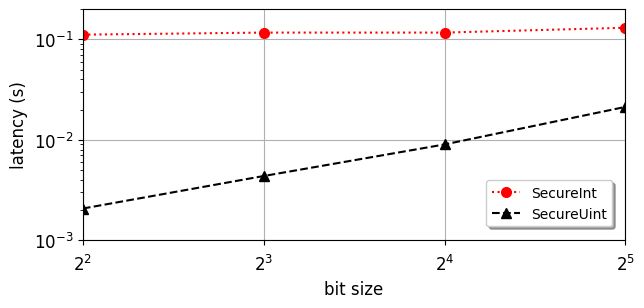
\includegraphics[width=\linewidth]{img/toSecureMod.png}}
	\caption{Conversion latency time from \secuint\ and \secint\ to \secmod\ for different bit sizes. Throughput is up to $n=2^{15}$ times faster since a ciphertext fits $n$ plaintexts.}
	\label{fig:tosecmod}
	\vspace{-0.6cm} 
\end{figure}

We also evaluate the conversion latency time from \secmod\ to \secuint/\secint\ using the algorithms presented in Listings \ref{list:secmod2secuint} and \ref{list:secmod2secint} with different plaintext moduli and bit sizes ($s = \{4, 8, 16, 32\}$). Fig.~\ref{fig:fromsecmod} summarizes the findings.
The results are what we expect from analysing the algorithms in Listings \ref{list:secmod2secuint} and \ref{list:secmod2secint}: When converting from \secmod\ to \secuint, the latency increases linearly to the bit size due to the operation on line 11 of Listing \ref{list:secmod2secuint}. Nevertheless, the dominant factor is the plaintext modulus $t$. A minor logarithmic effect comes from the exponentiation function (line 10) where the number of multiplications increases, while a major linear effect comes from the larger number of iterations in the \texttt{for} loop (line 7).
The conversion from \secmod\ to \secint\ (Listing \ref{list:secmod2secint}) takes roughly twice the time since it consists of two calls to the \secmod\ to \secuint\ conversion (lines 4 and 8) plus two multiplications (line 11).

\begin{figure}[t]
	\centering
    \frame{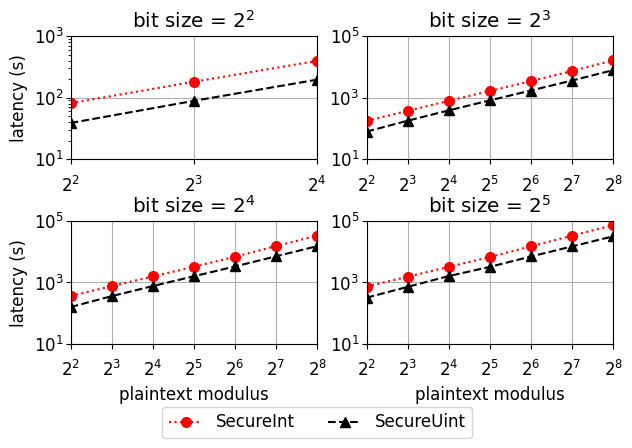
\includegraphics[width=\linewidth]{img/fromSecureMod.png}}
	\caption{Conversion latency time from \secmod\ to \secuint\ and \secint\ for different plaintext moduli and bit sizes.}
	\label{fig:fromsecmod}
	\vspace{-0.5cm}
\end{figure}



% \innersection{Insights}
% The results show that the conversion from bit-level to modular arithmetic is fast and can be used in practice. Meanwhile, converting from modular to bit-level arithmetic has borderline practical times only for very small plaintext moduli. With an small increase in the plaintext modulus, it quickly becomes prohibitive.

\subsection{Benchmarks}\label{ss:benchmarks}

In order to evaluate different execution modes (bit-level arithmetic and bridging), we use six data-oblivious benchmarks, some of which were adapted from the TERMinator Suite \cite{terminator}. \iffalse , while others were included based on their use in FHE applications. \fi These benchmarks are developed to be data-oblivious and manipulate sets of encrypted variables adjusted to $\{4, 8, 16\}$-bit size.
The algorithms are: (FIB) Fibonacci, an additive-intensive algorithm, (LOG) Logistic Regression, where the data must be capped before inference, (MAX) Maximum, commonly used as non-linear function in ML applications, (MUX) Multiplexer, a simple operation similar to the ternary operator that replaces branch conditions on encrypted data, (PKS) Private Keyword Search, which searches privately for an item in a list or database, and (SOR) Sort, a sorting algorithm with low multiplicative depth, designed for FHE.

% The algorithms are: (FIB) Fibonacci, an additive-intensive algorithm that we use as example in this manuscript, (LOG) Logistic Regression, where the data must be capped before inference, (MAX) Maximum, commonly used as non-linear function in machine learning applications, (MUX) Multiplexer, a simple operation similar to the ternary operator that replaces branch conditions on encrypted data, (PKS) Private Keyword Search, which searches privately for an item in a list or database, and (SOR) Sort, a sorting algorithm with low multiplicative depth specifically designed for FHE.
% The source code of all benchmarks with and without bridging is available in the Appendix.

\begin{figure}[t]
    % \vspace{-0.2cm}
	\centering
    \frame{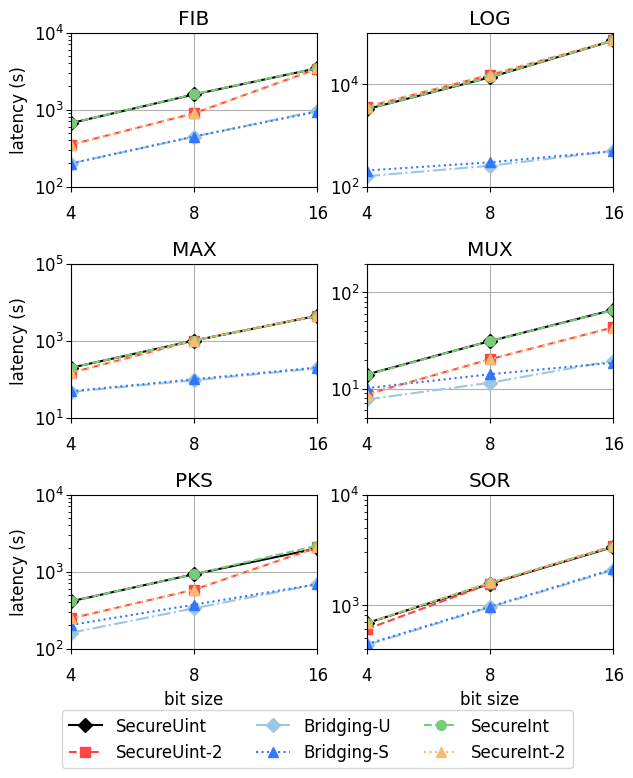
\includegraphics[width=\linewidth]{img/cases_latency.png}}
	\caption{Latency time for six benchmarks\iffalse using \secuint, \secint, unsigned and signed bridging, \texttt{Bridging-U} and \texttt{Bridging-S}, respectively,\fi with $t=2^{16}+1$. \iffalse In addition, we evaluate the benchmarks using \secuint\ and \secint\ with $t=2$ (postfix \texttt{-2}). \fi}
	\label{fig:benchmarks}
	\vspace{-0.4cm} 
\end{figure}

\innersection{Effect of plaintext modulus} Although $t=2$ does not enable batching in BFV, and therefore, it would not be used in practice, we compare it against the smallest plaintext modulus that enables batching ($t=2^{16}+1$) for $n=2^{15}$. The plaintext modulus does not affect the latency time to execute a homomorphic operation, but some homomorphic gates simplify in modulo 2 (e.g. XOR), as we discuss in Section \ref{ss:modcom}. Thus, a Boolean circuit used in bit-level arithmetic should have lower latency for $t=2$ if it contains XOR or XNOR gates. In Fig. \ref{fig:benchmarks}, we can see that in fact some applications are faster in modulo 2 (\texttt{SecureUint-2} and \texttt{SecureInt-2} for unsigned and signed bit-level arithmetic with $t=2$). MUX is the simplest benchmark, containing in bit-level arithmetic one equality, two \secbool-\secuint\ multiplications (or \secbool-\secint\ for signed numbers), one negation, and one addition. A \secbool-\secuint\ multiplication is entirely composed of XOR gates, and around half of the gates in the equality are XOR or XNOR. These operations are mainly responsible for the speed-up. 

% We have a similar situation for FIB and PKS, however here there are relatively fewer \secbool-\secuint\ multiplications and more additions, diminishing the effect of operating in modulo 2. The other benchmarks are much more complex applications and we noticed no difference in latency time between $t=2$ and $t=2^{16}+1$.

\innersection{Bit-level arithmetic vs bridging} Fig. \ref{fig:benchmarks} presents the latency time comparison between bit-level arithmetic and bridging. Regarding unsigned numbers (\secuint\ vs \texttt{Bridging-U}), results show that bridging outperforms bit-level arithmetic for all benchmarks and bit sizes. For some applications, like SOR, the performance improvement is limited (around 60\% speed-up). This happens because this algorithm requires many non-native operations (comparisons) in most stages. Only in the last part of the algorithm bridging can be employed, since using bridging before would require the inefficient conversion from \secmod\ to \secuint\ in order to execute the latter comparisons. Conversely, the logistic regression benefits a lot from using bridging with a speed-up of more than two orders of magnitude. This is possible because the non-native operations required by the filtering function are executed first. Therefore, at the filtering stage it is already possible to employ bridging and perform the remaining computation using the faster modular arithmetic.

\innersection{Signed numbers} Also in Fig. \ref{fig:benchmarks} we compare how bridging behaves with signed numbers. \iffalse In general, the extra conversion time required for signed numbers has little effect in the latency since the application uses significantly more multiplications compared to all the conversions. \fi We can see some degradation in PKS (4 bits) and MUX (4 and 8 bits). In PKS, there is conversion from \secint\ to \secmod\ in every iteration of the loop. The slowest operation in the loop is the comparison. This comparison operation is faster for smaller circuits (4 bits); therefore, the proportional latency of the two ciphertext multiplications required for the \secint\ to \secmod\ conversion is higher. For larger circuits, the comparison becomes more costly, thus, amortizing the conversion cost.

% Regarding MUX, it is a very simple function. It consists only of a comparison followed by a selection of one of two items. The explanation is similar to PKS, but the signed conversion has a higher impact in the latency time because there are two conversions instead of one in this algorithm.

\begin{figure}[t]
    % \vspace{-0.2cm}
	\centering
    \frame{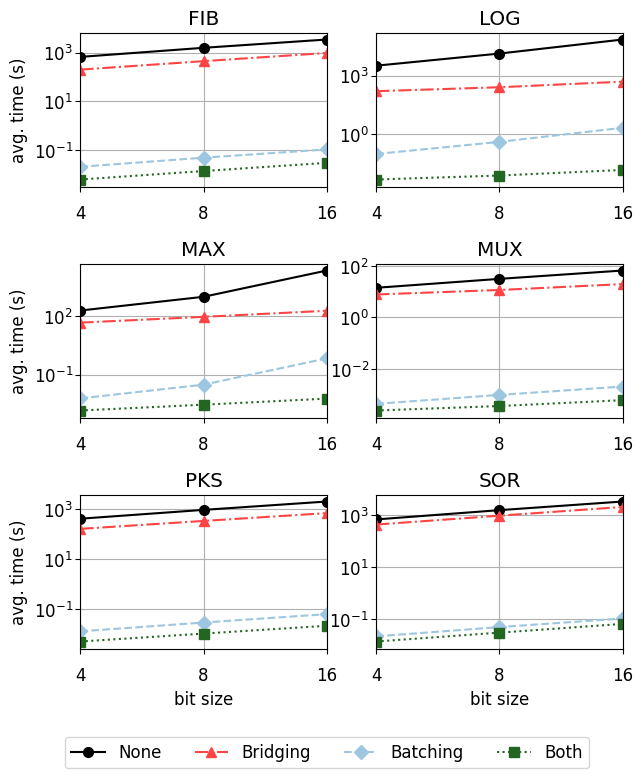
\includegraphics[width=\linewidth]{img/batching.png}}
	\caption{Average execution time for six benchmarks. \iffalse using and four cases: \texttt{None}: without bridging and batching, \texttt{Bridging}: with bridging only, \texttt{Batching}: with batching only, and \texttt{Both}: with both bridging and batching.\fi}
	\label{fig:batching}
	\vspace{-0.4cm} 
\end{figure}



\innersection{Bridging can be used with batching} Batching is a powerful technique used in FHE to pack many plaintexts into a ciphertext. The number of plaintexts that can be packed into a ciphertext is equal to the polynomial degree ($n = 2^{15}$ in our case). Although carefully crafted algorithms using batching and rotations can reduce program latency, the main benefit of batching is increased throughput, since it is possible to process $n$ plaintexts at once. Bridging on the other hand always reduces latency, and consequently improves throughput.
Bridging is a technique independent of batching and both can be used in tandem.
In Fig. \ref{fig:batching} we present the average execution time ($\text{latency} / \text{\# plaintexts packed}$) for six benchmarks and four cases: no batching and no bridging (\texttt{None}), bridging-only (\texttt{Bridging}), batching-only (\texttt{Batching}), and batching and bridging together (\texttt{Both}).
As expected, the throughput improvement provided by batching is impressive. However, for this technique to be used at its fullest, it is necessary to fill all ciphertext slots with plaintexts, which is the case with embarrassingly parallel workload. If the load is less than $n$, the performance will degrade.
Bridging does not suffer from this problem since it focuses on reducing the latency.
Nevertheless, bridging can be used in combination with batching. In this case, the speed-up of both techniques is added, leading to an even faster runtime (acceleration by more than 6 orders of magnitude (LOG)).

\innersection{Insights}
Bridging demonstrates substantial performance improvement for algorithms that allow mixing \secuint{} and \secmod{}, while in the worst case, bridging is equivalent to bit-level arithmetic. \iffalse This would happen if all outputs of a program come out from non-native operations. \fi
The comparison heavy SOR benefits less from bridging since these operations occur throughout the program and near the output, which precludes using the \secmod{} type in an earlier stage. On the contrary the benchmarks containing non-native operations near the beginning exhibit more significant performance improvements (MAX, FIB, PKS).
\iffalse At first glance, the MAX algorithm looks similar to SOR. However, some subtle differences in the \texttt{selection} function allow us to use bridging much earlier in the program; in fact, near the beginning of the application, leading to a much more noticeable performance improvement. 
FIB, and PKS have comparisons in all iterations, but since these comparisons are at the beginning of each iteration, bridging provides substantial performance improvements. \fi
Bridging benefits are maximized when non-native operations (e.g. comparisons) are at the beginning of the computation and the remaining of the computation can be done in modular arithmetic. The non-native operation would require the whole computation to work on bit-level arithmetic, but with bridging it becomes much faster since only the non-native operations are performed with \secuint, while the remaining run using \secmod. This is demonstrated by our logistic regression benchmark, which provides more than two orders of magnitude (precisely 143 times) of performance improvement.

% Finally, it is possible to combine bridging with batching for further performance improvement since both techniques are orthogonal to each other. It should be noted that this performance improvement is tightly connected to the parallelization capabilities of the workload. Nevertheless, results show that some benchmarks, when \emph{both} batching and bridging are combined, can be accelerated by more than 6 orders of magnitude (LOG).

\vspace{-0.1cm}
% \subsection{Case studies}\label{ss:cases}

% \subsubsection{URL denylisting}
\label{ss:url}
\begin{figure}[h!]
% \vspace{-0.2 cm}
\begin{minipage}{\linewidth}
\begin{lstlisting}[language=C++, caption={
Relevant function of the setup protocol of the URL denylisting application with bridging.
},
style=mystyle, 
label=list:pmt_sort,
xleftmargin=0.45cm,
% xrightmargin=-0.12\linewidth,
% linewidth=0.88\linewidth
]
template <int S> vector<SecureMod>
sort (int logt, vector<int> filter,
  const vector<SecureUint<S>> & order)
{
  using SecUint = SecureUint<S>;
  auto s = order.size();
  auto n = SecureMod::slots();
  auto nsp = n*s*logt;
  filter.resize(nsp, 0);
  vector<vector<unsigned>> f;
  for (int i=0; i<s; i++)
  {
    vector<unsigned> poly;
    for (int j=0; j<n; j++)
    {
      unsigned plain = 0;
      for (int k=0; k<logt; k++)
        plain = (plain<<1) +
          bool( filter[i+(j*logt+k)*s] );
      poly.push_back(plain);
    }
    f.push_back(poly);
  }
  
  $//$vector<SecUint> efilter;
  vector<SecureMod> efilter;
  for ( int i=0; i<s; i++ )
  {
    const auto & c = order[i];
    $//$vector<SecUint> partial_res;
    vector<SecureMod> partial_res;
    for (int j=0; j<s; j++)
    {
      $//$auto tmp = (c==j) * SecUint(f[j]);
      auto tmp = SecureMod(c==j) * f[j];
      partial_res.push_back(tmp);
    }
    $//$ low depth array summation  
    auto r = sum(partial_res);
    efilter.push_back(r);
  }
  return efilter;
}
\end{lstlisting}
\end{minipage}
\vspace{-0.6 cm}
% \vspace{-0.1 cm}
\end{figure}

We evaluate the performance improvements provided by bridging using a URL denylisting application as a case study \cite{urldenylist}.
The application implements a Private Membership Test (PMT) protocol, a common cryptographic building block for privacy-preserving applications.
Its main operation is checking if an element is part of a database without revealing information about the element.
In this scenario, the server hosting the database is semi-trusted (honest-but-curious).

URL denylisting is the process where a URL is being checked against a known database of malicious URLs; if there is a match, the access to the website is blocked. URL denylisting can be used in conjunction with URL rewriting to protect against e-mail phishing attacks. In other words, when an email comes to the company server, its URLs are being replaced by a redirection to the service provider site, which checks whether the link is malicious or not. If it is benign, the user is automatically forwarded to the webpage. While this (supposedly) protects against phishing attacks, it introduces a huge privacy problem, since the company hosting the service can clearly see which links the users are visiting, and can potentially sell the data to other parties. 

The PMT protocol we evaluate here is composed of two main phases: setup and query. In the setup phase, the database is converted into a format that enables fast queries. The query phase is simply checking if a particular element is part of the database.
While queries are fast, the setup is expensive since it uses comparison operations. As mentioned in the previous sections, comparisons require bit-level arithmetic, leading to execution times of more than a day for databases with millions of entries. Implementing a faster setup protocol is therefore critical to the practicality of the application. 

The setup protocol is composed of three main stages: 1) The server database containing the list of malicious URLs is converted into a Bloom filter \cite{bloomfilter}. The server then informs the size of this Bloom filter $m$ to the client. 2) In the next step, the client creates a list with random permutations of \mbox{$\ceil{ {m}/({n \cdot \floor{\log_{2}{t}}} ) }$} unique integers, where $m$ is the size of the Bloom filter, $n$ is the polynomial degree, and $t$ is the plaintext modulus. The client encrypts the list with its public key and sends to the server. 3) Finally, the server runs a particular homomorphic algorithm that sorts the Bloom filter into a way only known to the client. This produces an encrypted Bloom filter in this particular order.

Out of the three stages in the setup, only the third one operates homomorphically on encrypted data. Therefore, we implemented the third stage of the setup protocol using bridging and compared its performance against the bit-level arithmetic implementation.
As shown in Fig. \ref{fig:application}, bridging provides approximately one order of magnitude of performance improvement for this application, reducing the setup time for databases with one million entries to less than three hours, instead of more than a day when bit-level arithmetic is exclusively used.

\begin{figure}[t]
	\centering
    \frame{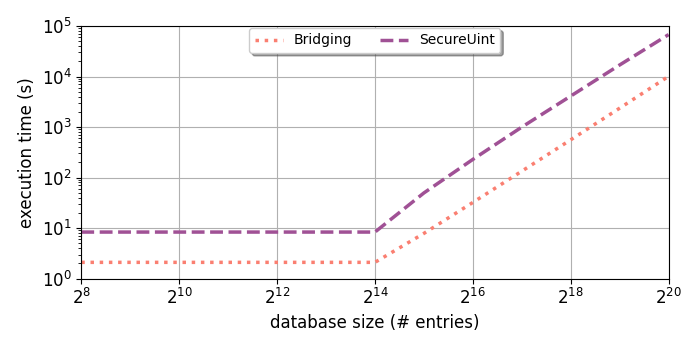
\includegraphics[width=\linewidth]{img/application.png}}
	\caption{Execution time of the setup protocol of a URL denylisting application \cite{urldenylist} implementing the Private Membership Test.}
	\label{fig:application}
\end{figure}

This performance improvement is enabled with just a few tweaks to the sort algorithm.
Consider Listing \ref{list:pmt_sort} presenting this algorithm as an example of modifications required to enable bridged computation.
Function \texttt{sort} reorders the items of a Bloom filter in a sequence known only to the client using encrypted variable \texttt{order}. It creates a list of plaintext indices according to the protocol (lines 10-23), compares homomorphically with the encrypted list of unique permutations sent by the client (variable \texttt{order}), and composes the encrypted Bloom filter \texttt{efilter} with values in this particular order (lines 25-42).

The homomorphic operations start after line 24. There are only a few necessary changes to the algorithm: 1) In lines 1, 26, and 31 we change the return and variable types from \texttt{vector<\secuint<S>{}>} to \texttt{vector<\secmod>}, and 2) in line 35, we cast the \secbool\ type to \secmod, so the subsequent multiplication is done using modular arithmetic.
In bit-level arithmetic it is faster to cast the \texttt{vector<int>} to \secuint\ and multiply by a \secbool, since it results in a \secbool-\secuint\ multiplication instead of a \secuint-\texttt{vector<int>} multiplication. Nevertheless, with bridging it is faster to cast the \secbool\ to \secmod, instead of \texttt{vector<int>}, because \secmod-\texttt{vector<int>} multiplication is faster and less noisy than \secmod-\secmod\ multiplication.
As can be seen in Fig. \ref{fig:application}, Bridging unlocks {\it one order of magnitude} performance improvement, and it only requires minor changes to the source code.

% \subsubsection{Genotype imputation}\label{sss:genotype}
\subsection{Case-study: Genotype imputation}\label{sss:genotype}

Genotype imputation is the process of filling missing information in DNA sequencing with the use of statistical methods. \iffalse Due to the computer-intensive nature of the task, cloud servers are a natural platform for processing the data. Furthermore, privacy requirements of medical information make solutions using homomorphic encryption desirable. \fi P-Impute \cite{GURSOY2021} converts an inefficient statistical model based on correlation of similar individuals %\footnote{The similarity of individuals is determined based on matching single-nucleotide polymorphisms (SNPs) in proximity to the missing SNP.}
into a Private Information Retrieval (PIR) problem, which has efficient solutions in FHE, using the BFV encryption scheme. In this section, we discuss the performance of p-Impute without (\secuint) and with bridging taking into consideration the multiplicative depth for defining more efficient encryption parameters. Batching is used to fit $n$ plaintexts into a ciphertext.

% As this application has much higher memory requirements compared to the previous experiments, we ran the experiments on an Intel Xeon Silver 4214R CPU @ 2.40GHz with 24 cores and 1 TB of memory running on RHEL 7.9. We use the same version of E3 and Microsoft SEAL as in the other experiments with GCC 7.3.1.
We set each run to use 24 threads and report the query time, i.e., the time performing encrypted computation, and the number of ciphertext additions, multiplications, and subtractions in Table \ref{tab:nops}. We use the same plaintext modulus as in the other experiments ($t = 2^{16}+1$), but we vary the polynomial degree ($n \in \{2^{13}, 2^{14}, 2^{15}\}$) in order to evaluate the extra performance improvement provided by bridging for requiring a lower multiplicative depth.
Without bridging, we were only able to run with $n = 2^{15}$, since lower polynomial degrees do not provide enough noise budget to run the application without bootstrapping. %\footnote{Bootstrapping is not supported by Microsoft SEAL library. Accounting for noise growth is commonly tasked to the programmer in FHE applications.}
With bridging, we were able to reduce $n$ to $2^{13}$ without corrupting the result.
As $n$ reduces, the number of batching slots in a ciphertext reduces since it is equal to the polynomial degree. However, the reduction in latency for the homomorphic operation compensates for the reduction in slots. Experimental results show that when $n$ is halved, the latency of the ciphertext multiplication reduces by at least 4 times, and can be amplified depending on the behavior of cache memories. \iffalse This effect can be even greater due to effects related to cache memories.  Therefore, reducing the polynomial degree is always desirable.\fi Consequently, one halving of $n$ increases throughput by at least 2x and reduces latency by 4x.

For the same polynomial degree ($n = 2^{15}$), bridging is around 6.82x faster than bit-level arithmetic. This is due to the reduced number of operations on encrypted data, as one can see in Table \ref{tab:nops}.
Nevertheless, bridging requires less noise budget to operate, which allows us to use smaller polynomial degrees. In the fastest case, bridging has the throughput improved by 62.2x, while the latency reduces by around 249 times.
\vspace{-0.1cm}
\begin{table}[t]
    \centering
    \caption{Number of ciphertext \iffalse additions, multiplications, and subtractions, \fi operations and execution time for p-Impute \cite{GURSOY2021}. \iffalse with and without bridging \replace[and]{using} different polynomial degrees (n).  Without bridging, only $n = 2^{15}$ has enough noise budget for the computation. \fi}
    \vspace{-0.4cm}
    \begin{tabular}{crrrrr}
        Bridging & n &  add  &  mul  &  sub  & time (s) \\ \hline
        \normalfont{no}  & \unboldmath \( 2^{15} \) & \normalfont{53288} & \normalfont{66152} & \normalfont{51256} & \normalfont{5026} \\ \hline
        \normalfont{yes} & \unboldmath \( 2^{15} \) & \normalfont{14248} & \normalfont{ 9072} & \normalfont{ 4536} & \normalfont{ 737} \\ \hline
        \normalfont{no} & \unboldmath \( 2^{14} \) & \normalfont{ NA} & \normalfont{ NA} & \normalfont{ NA} & \normalfont{ NA} \\ 
        \hline
        \normalfont{yes} & \unboldmath \( 2^{14} \) & \normalfont{28496} & \normalfont{18144} & \normalfont{ 9072} & \normalfont{ 196} \\ 
        \hline  
        \normalfont{no} & \unboldmath \( 2^{13} \) & \normalfont{ NA} & \normalfont{ NA} & \normalfont{ NA} & \normalfont{ NA} \\ 
        \hline
        \normalfont{yes} & \unboldmath \( 2^{13} \) & \normalfont{56992} & \normalfont{36288} & \normalfont{18144} & \normalfont{  80} \\ 
             
    \end{tabular}
    \label{tab:nops}
    \vspace{-0.5cm}
\end{table}


% \begin{table*}[!th]
\centering
\begin{tabular}{cc|ccc|ccc|cc|cc}
  &   & \multicolumn{3}{c|}{\secuint\ \texttt{to} } & \multicolumn{3}{c|}{\secint\ \texttt{to} } & \multicolumn{2}{c|}{\secmod\ \texttt{to} } & \multicolumn{2}{l}{\secmod\ \texttt{to} } \\ 
  \multicolumn{1}{c}{} & \multicolumn{1}{c|}{} & \multicolumn{3}{c|}{\secmod{}}        & \multicolumn{3}{c|}{\secmod{}}      & \multicolumn{2}{c|}{\secuint{}}     & \multicolumn{2}{c}{\secint{}}     \\ \hline
s  & t & mul     & add     & depth    & mul     & add    & depth    & mul            & depth         & mul           & depth        \\ \hline
\normalfont{4}  & \unboldmath \( 2^{4} +1 \)  & \normalfont{0}         & \normalfont{6}         & \normalfont{0}       & \normalfont{2}         & \normalfont{9}        & \normalfont{1}       & \normalfont{136}              & \normalfont{5}            & \normalfont{274}             & \normalfont{6}           \\ \hline
\normalfont{7}  & \unboldmath \( 2^{7} +1 \)  & \normalfont{0}         & \normalfont{12}        & \normalfont{0}       & \normalfont{2}         & \normalfont{15}       & \normalfont{1}       & \normalfont{1778}             & \normalfont{8}            & \normalfont{3558}            & \normalfont{9}           \\ \hline
\normalfont{8}  & \unboldmath \( 2^{16} +1 \)  & \normalfont{0}         & \normalfont{14}        & \normalfont{0}       & \normalfont{2}         & \normalfont{17}       & \normalfont{1}       & \normalfont{1572888}          & \normalfont{17}           & \normalfont{3145778}         & \normalfont{18}          \\ \hline
\normalfont{16} & \unboldmath \( 2^{16} +1 \)  & \normalfont{0}         & \normalfont{30}        & \normalfont{0}       & \normalfont{2}         & \normalfont{33}       & \normalfont{1}       & \normalfont{2097184}          & \normalfont{17}           & \normalfont{4194370}         & \normalfont{18}         \\
\end{tabular}
\caption{Number of ciphertext additions and multiplications, and multiplicative depth for converting from \secuint\ and \secint\ to \secmod, and vice-versa. The results show that \secmod{} to \secuint\ and \secint\ conversion is impractical. The overhead from ciphertext additions for converting from \secmod\ to \secuint\ and \secint\ is negligible and not included.}
\label{tab:conversion}
\end{table*}



% \begin{table}[t]
    \centering
    \begin{tabular}{c|c|c}
         \review{\secuint{}}                & \review{mul}   & \review{\normalfont{0}}                                                           \\
         \review{\normalfont{to}}           & \review{add}   & \review{\normalfont{$2 \cdot (s - 1)$}}                                           \\
         \review{\secmod{}}                 & \review{depth} & \review{\normalfont{0}}                                                           \\ \hline
         \review{\secint{}}                 & \review{mul}   & \review{\normalfont{2}}                                                           \\
         \review{\normalfont{to}}           & \review{add}   & \review{\normalfont{$2s + 1$}}                                                    \\
         \review{\secmod{}}                 & \review{depth} & \review{\normalfont{1}}                                                           \\ \hline
         \review{\secmod{} \normalfont{to}} & \review{mul}   & \review{\tiny{$t \cdot (s + \floor{\log_2{(t-1)}} + \omega(t-1) - 1)$}}           \\
         \review{\secuint{}}                & \review{depth} & \review{\scriptsize{$\ceil{\log_2{(t-1)}} + 1$}}                                  \\ \hline
         \review{\secmod{} \normalfont{to}} & \review{mul}   & \review{\tiny{$2 \cdot t \cdot (s + \floor{\log_2{(t-1)}} + \omega(t-1) - 1)+2$}} \\
         \review{\secint{}}                 & \review{depth} & \review{\scriptsize{$\ceil{\log_2{(t-1)}} + 2$}}                                  \\
    \end{tabular}
    \caption{\review{General terms for the number of multiplications (mul), number of additions (add), and multiplicative depth (depth) for converting from \secuint\ and \secint\ to \secmod\ and vice-versa, where $s$ is the number of encrypted bits in the \secuint/\secint\ variable, $t$ is the plaintext modulus, and $\omega(\cdot)$ is the Hamming weight.}}
    \label{tab:general}
\end{table}


\subsubsection{\secmod\ to \secint{}}\label{sss:secmod2secint}

Conversion from \secmod\ to \secint\ is possible by applying Eq. \ref{eq:secmod2secint} to the result of Eq. \ref{eq:secmod2secuint}:
\begin{equation}\label{eq:secmod2secint}
    Y = (1 - X_{s-1}) \cdot X + X_{s-1} \cdot (2^s - t + X)
\end{equation}
$X$ is the result of Eq. \ref{eq:secmod2secuint}, $Y$ is the \secint\ output, $s$ is the number of encrypted bits in $X$ and $Y$, $t$ is the plaintext modulus, and $2^s \geq t$.
Listing \ref{list:secmod2secint} shows the algorithm for this conversion. It leverages the conversion described in Listing \ref{list:secmod2secuint} and adjusts for the sign.
This algorithm requires $2 \cdot t \cdot (s + \floor{\log_2{(t-1)}} + \omega(t-1) - 1)+2$ multiplications with a multiplicative depth of $\ceil{\log_2{(t-1)}} + 2$.

\begin{figure}[!t]
%\scriptsize
\begin{minipage}{\linewidth}
\begin{lstlisting}[language=C++, caption={
Casting from \secmod\ to \secint.}, style=mystyleb, label=list:secmod2secint,
%framexrightmargin=-37pt,
% xleftmargin=0.4cm,
% xrightmargin=-0.12\linewidth,
% linewidth=0.88\linewidth
]
template <int Size>
SecureInt to_SecureInt<Size>(SecureMod x)
{
    auto u = to_SecureUint<Size>(x);
    SecureInt<Size> pos(u);
    auto max = 1 << s;
    auto diff = max - SecureMod::t;
    u = to_SecureUint<Size>(diff + x);
    SecureInt<Size> neg(u);
    auto & isNeg = pos[s-1];
    return isNeg * neg + (1-isNeg) * pos;
}
\end{lstlisting}
\end{minipage}
% \vspace{\lstbspace}
\vspace{-0.5cm} 

\end{figure}

\section{Proposed Bridging Methodology}\label{s:bridging}

We define new data types to abstract the low-level complexity of the encryption scheme and Boolean circuits.
This is possible by extending the  E3 framework \cite{e3eprint}, which is one level of abstraction above FHE libraries and enables portability of code across different libraries.
% \vspace{-0.4cm}
\subsection{Modular and bit-level arithmetic}\label{ss:modcom}

Some FHE schemes define arithmetic addition, subtraction, and multiplication on numeric rings, but not other arithmetic such as division or comparison. While some applications may not require any other operation, a programmer is accustomed to having all programming operations available in their programs.
For example, the C++ statement "{\tt{}if(a<b)c+=a}" and its corresponding data-oblivious form: "{\tt{}c+=(a<b)*a}", cannot be evaluated with an FHE scheme where the comparison operation is not defined.
Notably, addition, subtraction, and multiplication on integers is an incomplete set of arithmetic operations; for instance, the comparison operation cannot be reduced to these three operations. However, when operating on bits, the same set of operations is universal, having addition and subtraction correspond to logical \texttt{XOR} and multiplication to logical \texttt{AND}.

\eee\ solves this problem by allowing the programmer to use data types constructed out of sequences of encrypted bits. Indeed, as the least possible requirement to the computing capacity, an FHE scheme must be able to evaluate the logic \texttt{NAND} (or \texttt{NOR}) gate on ciphertexts, since this elementary function is sufficient for universal computation. 
In this way, the variables in the expression "{\tt{}c+=(a<b)*a}" are defined as \emph{integral types} where all three operations (comparison, multiplication, and addition) are performed using bit-level arithmetic circuits. We call this computation {\it bit-level arithmetic}, as opposed to the natively provided {\it modular arithmetic}, where addition and multiplication are performed directly on ciphertexts.

The transition from modular to bit-level arithmetic is straightforward: Since
the encrypted bit values are limited to 0 and~1, logic gates, such as \texttt{AND}, \texttt{XOR}, \texttt{NOT}, etc, can be expressed via the following expressions:
\vspace{-0.2cm}
\begin{equation*}\label{eq:logic}
\begin{split}
x \ \texttt{AND} \ y = xy,& \qquad x \ \texttt{NAND} \ y = 1-xy \\
x \ \texttt{OR} \ y = x+y-xy,& \qquad x \ \texttt{NOR} \ y = 1-(x \ \texttt{OR} \ y) \\
x \ \texttt{XOR} \ y = x+y-2xy,& \qquad x \ \texttt{XNOR} \ y = 1-(x \ \texttt{XOR} \ y) \\
 \texttt{NOT} \ x = 1-x,& \qquad \texttt{MUX}(x,y,z) = x(y-z)+z, \\
\end{split}
\end{equation*}

\noindent where \texttt{MUX} is the multiplexer operation (as in {$x$?$y$:$z$}). The set of values $\{0,1\}$ is closed under the above set of expressions. 
In this paper, we use the term \emph{homomorphic gates} to describe logic gates operating on encrypted bits. Given these homomorphic gates, higher level operations (comparison, addition, multiplication) can be built using standard combinational arithmetic circuit design, which allows to perform any programming operation, i.e. giving the full spectrum of C++ arithmetic. Gate equations simplify for plaintext modulo $2$; e.g. XOR gate does not require multiplication, as \mbox{$x \ \texttt{XOR} \ y = x+y \bmod 2$}.

\innersection{Data types}
We define three data types for bit-level arithmetic, \secuint, \secint, and \secbool, and one for modular arithmetic, \secmod. 
A \secuint\ or \secint\ variable is an array of ciphertexts, each encrypting either zero or one. \secuint\ is comparable to \texttt{unsigned int}, while \secint\ corresponds to \texttt{int}.
The third type is \secbool, which is a type derived from \secuint\texttt{<1>}. It is the secure equivalent of \texttt{bool}.
For modular arithmetic, there is only the native type, which operates modulo the plaintext modulus. We call this type \secmod.

With bit-level arithmetic, we can express programs with operations not supported by modular arithmetic.
Listing~\ref{list:fibs} demonstrates the transition from plaintext computation to secure computation: Integer variables are declared with the secure type \secuint; the rest of the code remains the same.
%\footnote{\secuint\ is the secure equivalent of \texttt{unsigned int}. We discuss signed integers later.} Note that the type is parameterized with the size. 
In encrypted computation, increasing the number of bits of integral types can lead to a dramatic increase in performance overhead.
For this reason, we define the bit size as a template specialization.
% As experimental results demonstrate, even 1 bit can make significant difference in performance, affecting the practicality dimension. 
Explicit size declaration can be found in functional programming languages, so the programmer may already be familiar with this practice.
In the example of Listing~\ref{list:fibs}, all variables are 8 bits (lines 3, 4).

The postfix {\tt{}\_E} after each constant provides encrypted values used in variable initialization of integral type variables.
% The configuration file with the specifications of the encryption defines the type name and postfix used for constants in the program.
\eee\ automatically encrypts and replaces the plaintext constants with their encrypted representations, so the final binary does not have information about the initial values used in the program. 

\begin{figure}
%\scriptsize
\begin{minipage}{\linewidth}
\begin{lstlisting}[language=C++, caption={Secure version of Fibonacci function. Type \secuint\ behaves as native {\tt unsigned int}.
% \hspace{-1.40cm} \mbox{}
}, style=mystyle, label=list:fibs,
% xrightmargin=-0.12\linewidth,
% linewidth=0.96\linewidth
]
SecureUint<8> fibonacci(SecureUint<8> in)
{
    SecureUint<8> i=_0_E, a=_0_E, b=_1_E;
    SecureUint<8> r=_0_E;
    int max_iter = 10;
    while( max_iter-- )
    {
        r += (i++ == in) * a;
        std::swap(a,b);
        a += b;
    }
    return r;
}
\end{lstlisting}

\vspace{-0.5cm} 

% \vspace{0.2in}

% \begin{lstlisting}[language=C++, caption={An outline example of \secint\ definition.
% % \hspace{-1.40cm} \mbox{}
% }, style=mystyle, label=list:ciro,
% % xrightmargin=-0.12\linewidth,
% % linewidth=0.96\linewidth
% ]
% template <int Size> class SecureUint{ ... };
% constexpr std::string operator""_E
%   (unsigned long long int x){ ... }
% \end{lstlisting}
\end{minipage}
% \vspace{\lstbspace}
% \vspace{-0.8cm}
\end{figure}



\subsection{Bridging modular and bit-level arithmetic}\label{ss:bridging}

Declaring variables with a protected integral type and using solely bit-level arithmetic as in Listing~\ref{list:fibs} has a potential drawback: When an FHE scheme provides fast modular arithmetic operations, the usage of circuits operating on separate bits is slow. This paper brings the  idea of 
\textit{Bridging} - mixing both modular and bit-level arithmetic in one program with the ability to convert variables from one type to the other. %integral type to modular.
Some variables can be declared using a protected type supporting only modular arithmetic, while others with another secure type supporting bit-level arithmetic. In bridging mode, a type of bit-level arithmetic declares a conversion function into a type of modular arithmetic, and vice-versa.
In all cases, the encryption of the two different C++ types must share the same FHE keys, which is ensured by our proposed methodology and framework. 

\subsubsection{\secuint\ to \secmod{}}\label{sss:secuint2secmod}

For performance reasons, it is desirable to execute the entire computation in modular arithmetic, since it is much faster than bit-level. If however, a program requires an operation not supported in modular arithmetic (e.g., comparison), then, without Bridging, the whole program must perform all computations using bit-level arithmetic, severely degrading performance. 
In effect, Bridging enables the isolation of the parts of the computation requiring bit-level arithmetic.
For example, the expression "{\tt{}c+=(a<b)*a}" can use bit-level arithmetic for the comparison only.
The variables required by the comparison (i.e., \texttt{a} and \texttt{b}) must be of integral type. Nevertheless, the operands of the multiplication can be cast to our modular type, allowing multiplication and addition to be executed in modular arithmetic, resulting in a variable {\tt{}c} of modular type.

\begin{figure}
%\scriptsize
\begin{minipage}{\linewidth}
\begin{lstlisting}[language=C++, caption={
Bridging (i.e.,~mixing \secmod{} and \secuint\ types) enables performance improvement. The postfix \texttt{\_M} denotes encrypted variable for the \secmod\ type.
},
style=mystyle, 
label=list:fibm,
xleftmargin=0.45cm,
% xrightmargin=-0.12\linewidth,
% linewidth=0.88\linewidth
]
SecureMod fibonacci(SecureUint<8> in)
{
    SecureUint<8> i=_0_E;
    SecureMod a=_0_M, b=_1_M, r=_0_M;
    int max_iter = 10;
    while( max_iter-- )
    {
        r += (i++ == in) * a;
        std::swap(a,b);
        a += b;
    }
    return r;
}
\end{lstlisting}
\end{minipage}
% \vspace{\lstbspace}
\vspace{-0.8cm}

\end{figure}
% \vspace{-1cm} 

Listing~\ref{list:fibm} demonstrates the code of the Fibonacci function of Listing~\ref{list:fibs} with \emph{Bridged} arithmetic: Only the input \texttt{in} and counter \texttt{i} are declared as integral type \secuint{}, while the others are replaced with the faster \secmod\ type. 
Line 8 does implicit conversion from \secuint\ to \secmod;
in this way, bit-level multiplication (which is slow) is not executed. Instead, only the native (much faster) multiplication of ciphertexts is needed.
Specifically, the comparison between {\tt i} and {\tt in} is the slowest operation in the program, and its result is one encrypted bit which can naturally be casted to \secmod, since the set $\{0,1\}$ is a subset of the plaintext range.
The operation for casting an integral type (bit-level) into modular (FHE native) is a summation of the encrypted bits of the integral type. 
In fact, the binary representation of a value $X$ can be reorganized by {\it Horner's scheme} in a set of additions over its $s$ bits $x_i$:
\begin{equation*}
\begin{split}
X & = 2^{s-1}x_{s-1} +2^{s-2}x_{s-2} + ... + 2x_1+x_0 = \\
& =(...((x_{s-1})\cdot 2+x_{s-2})\cdot 2+...+x_1)\cdot 2+x_0
\end{split}
\end{equation*}

Evaluating the right hand side of the above equation yields the value corresponding to the bit sequence. This evaluation is an efficient way to convert a program variable of type \secuint{} into a \secmod{} value.
Listing~\ref{list:secuint2secmod} shows the C++ implementation of such casting.
We emphasize that this conversion requires no ciphertext multiplications, only additions. Specifically, $2 \cdot (s - 1)$ ciphertext additions with a maximum additive depth of $s-1$, where $s$ is the number of encrypted bits.

\begin{figure}[t]
%\scriptsize
\begin{minipage}{\linewidth}
\begin{lstlisting}[language=C++, caption={
Casting from \secuint\ to \secmod. Since the former is a set of ciphertexts representing encrypted bits, it is possible to access each bit individually.}, style=mystyleb, label=list:secuint2secmod,
%framexrightmargin=-37pt,
% xleftmargin=0.4cm,
% xrightmargin=-0.12\linewidth,
% linewidth=0.88\linewidth
]
template <int Size>
SecureMod to_SecureMod(SecureUint<Size> v)
{
    auto i = Size;
    SecureMod r = v[--i];
    while ( i-- ) r += r + v[i];
    return r;
}
\end{lstlisting}
\end{minipage}
% \vspace{\lstbspace}
\vspace{-0.5cm} 
\end{figure}

\begin{figure}[t]
%\scriptsize
\begin{minipage}{\linewidth}
\begin{lstlisting}[language=C++, caption={
Casting from \secint\ to \secmod. The \secint\ variable is converted to \secuint, which is then converted to \secmod.}, style=mystyleb, label=list:secint2secmod,
%framexrightmargin=-37pt,
% xleftmargin=0.4cm,
% xrightmargin=-0.12\linewidth,
% linewidth=0.88\linewidth
]
template <int Size>
SecureMod to_SecureMod(SecureInt<Size> v)
{
    SecureUint<Size> u(v);
    auto pos = to_SecureMod(u);
    int max = 1 << Size;
    auto neg = SecureMod::t - max + pos;
    SecureMod isNeg = v[Size-1];
    return isNeg * neg + (1-isNeg) * pos;
}
\end{lstlisting}
\end{minipage}
% \vspace{\lstbspace}
\vspace{-0.7cm} 
\end{figure}


% \iffalse Then, we use the most significant bit of the \secint\ variable to define whether the value is negative. \if 

Line 8 of Listing~\ref{list:fibm} does implicit conversion of \secbool{} to \secmod{}. Note that \secbool\ is a derived class from \secuint\texttt{<1>}. To observe a more complex scenario, consider the expression "{\tt{}c+=(a==b)*a}" that actually requires conversion of \secuint{}.
Comparison between \texttt{a} and \texttt{b} must be evaluated in bit-level. This implies that types of \texttt{a} and \texttt{b} must be \secuint{}. The comparison is done on a bit-by-bit manner using homomorphic gates following the gate equations described in Section \ref{ss:modcom}.
The gates correspond to normal logic gates, but operating on ciphertexts instead of ordinary bits. The result of the comparison is one encrypted bit represented by type \secbool.
Multiplication between a \secbool\ and a \secuint\ is evaluated as a multiplexer operation with $s$ \texttt{AND} gates, where $s$ is the number of encrypted bits in the \secuint\ variable, resulting in a \secuint{} type.
The type of variable \texttt{c} can be chosen as \secmod{}. The addition in the expression is then performed on variables of \secmod{} and \secuint{} types: "{\tt{}c=c+t}", where "{\tt{}t=(a==b)*a}". Implicit conversion evokes our function of Listing \ref{list:secuint2secmod} from the constructor of \secmod{} type out of \secuint{}.
Then the addition operation follows on two variables, both of the \secmod{} type.

It should be noted that all these conversions and evaluations are done obliviously to the user and do not require special attention; the user writes only "{\tt{}c+=(a==b)*a}".
A more efficient way to perform this computation is to explicitly convert argument \texttt{a}  in this expression to \secmod. In such case, the multiplication is done in modular arithmetic which is around $s$ times faster than a multiplication between \secbool{} and \secuint{} (and many more times faster than multiplying two \secuint{}s).\footnote{The exact speed-up compared to multiplying two \secuint s depends on the variables' bit size.} The corresponding expression becomes \mbox{"{\tt{}c+=(a==b)*\secmod(a)}"}.
Same way as above, the constructor calls the conversion function (Listing~\ref{list:secuint2secmod}), this time one step earlier - before the multiplication - resulting in having a larger portion of the computation in modular arithmetic, hence improving the performance.
It it worth noting that while there is automatic conversion from \secuint\ to \secmod, it is the programmer's task to define each variable's type and, in some cases, call conversion explicitly for better performance.

\subsubsection{\secint\ to \secmod{}}\label{sss:secint2secmod}

So far, we have discussed unsigned numbers. However, bit-level arithmetic also supports signed numbers following the two's complement arithmetic.
On the other hand, modular arithmetic only supports numbers in $\mathbb{Z}_t$, where $t$ is the plaintext modulus.
Nevertheless, it is possible to emulate negative numbers in modular arithmetic in the programmer's domain as in Cryptoleq \cite{cryptoleq}, where lower values are considered positive and large values are interpreted as negative numbers.
In this case, the conversion from a signed bit-level arithmetic type \secint\ to \secmod\ is defined as:
\begin{equation}
  X=\begin{cases}
    t - 2^s + \sum_{i=0}^{s-1}{(2^i \cdot x_i)}, & \text{if $x<0$}.\\
    \sum_{i=0}^{s-1}{(2^i \cdot x_i)}, & \text{otherwise}.
  \end{cases}
\end{equation}
where $s$ is the number of bits and $x_i$ is the bit of $x$ at position $i$. The condition $x < 0$ is determined by the most significant bit of $x$; thus, we can use it as a multiplexer between the two cases.
Listing \ref{list:secint2secmod} presents the algorithm for converting a \secint\ into a \secmod. First, the \secint\ is interpreted as a \secuint\ (line 4). In line 5, this value is converted into a \secmod\ using the algorithm of Listing \ref{list:secuint2secmod}.
Then in line 7, we perform the subtraction of plaintexts $t$ and \texttt{max} (i.e. $2^s$), and then do a ciphertext addition with the \secmod\ variable \texttt{pos}. At this point, we have generated two \secmod\ variables: \texttt{pos}, representing the value in case it is positive, and \texttt{neg} containing the value in case it is a negative number. This totals $2s - 1$ ciphertext additions with a additive depth of $s$.
Finally, we select between \texttt{neg} and \texttt{pos} using the most significant bit of the \secint\ input (lines 8-9). If the bit is one, it means it is a negative number; thus, we select \texttt{neg}; otherwise, we select \texttt{pos}.
For selection we need ciphertext multiplications.
The entire conversion from \secint\ to \secmod\ requires two ciphertext multiplications and $2s + 1$ ciphertext additions with a multiplicative depth equal to one.
By comparing Listings \ref{list:secuint2secmod} and \ref{list:secint2secmod}, we can see that converting signed numbers to \secmod\ is less efficient than converting unsigned numbers to \secmod. Furthermore, $t$ must be large enough ($t \geq 2^s$) to accommodate the converted value.

% \innersection{Why not signed and unsigned \secmod{}} \secmod{} types can only participate in addition, subtraction, and multiplication operations. The values of this type are elements of the corresponding mathematical ring. The programmer can choose to interpret a subset of the number space as negative, but there would be no difference in these computations. For this reason, there is no differentiation between the signed and unsigned versions for \secmod{} type.
\subsubsection{\secmod\ to \secuint{}}\label{sss:secmod2secuint}
\vspace{-0.2cm}
Conversion from \secmod\ to \secuint\ is theoretically possible using the expression:
\vspace{-0.2cm}
\begin{equation}\label{eq:secmod2secuint}
    \vspace{-0.1cm}
    X = \sum_{i=1}^{t-1}(i \cdot \secbool(1 - (x-i)^{t-1}))
\end{equation}
where $x$ is the \secmod\ variable to be converted, $t$ is the plaintext modulus and is prime, $i$ is a \secuint\ counter, and $X$ is the resulting \secuint. Due to the properties of modular arithmetic and the parameters used in homomorphic encryption, the exponentiation to $t-1$ results in zero in case the base is zero, and one otherwise. When $i = x$, the expression in the summation results in $i$, while in all other cases it will result in zero, since $1 - (x-i)^{t-1} = 0 \ \forall \ i \ne x$.
% Breaking down Eq. \ref{eq:secmod2secuint}:
% \begin{enumerate}
%     \item The \secuint\ $i$ is automatically cast to \secmod\ in $x-i$ before the exponentiation, resulting in a subtraction between two \secmod{}s.
%     \item The exponentiation of the \secmod\ $x-i$ to the integer $t-1$ results in a \secmod\ variable containing either the encryption of zero or one.
%     \item The result of the exponentiation is negated by subtracting it from one. At this point, we have the encryption of one in case $x = i$ and zero otherwise stored in a \secmod\ variable. In order to avoid automatically casting $i$ to \secmod\ in the multiplication, we must first reinterpret the partial result as \secbool.
%     \item We multiply the \secuint\ $i$ by the \secbool\ value resulting in a \secuint\ equal to $i$ or zero. We remark that a \secbool-\secuint\ multiplication is evaluated as a multiplexer operation.
%     \item We repeat this process for all $i \in [1,t)$, adding the resulting values. The final result is a \secuint\ equal to $x$ since there is only one $i$ that is equal to $x$.
% \end{enumerate}

An implementation of the fast exponentiation algorithm is presented in Listing \ref{list:pow}. The number of multiplications is given by $\floor{\log_2{e}} + \omega(e) - 1$ and the multiplicative depth is $\ceil{\log_2{e}}$, where $e$ is the exponent and $\omega(\cdot)$ is a function that calculates the Hamming weight. The conversion from \secmod\ to \secuint\ can exploit this property of the exponentiation to $t-1$ resulting in zero or one to create an equality function, where the equality function is given by $1 - (x-i)^{t-1}$. With this information, we can build a linear search to find the \secuint\ $i$ that is equal to the \secmod\ $x$ using the result of the equality as a selector. Listing \ref{list:secmod2secuint} presents the algorithm that performs this conversion.
The number of multiplications is given by $t \cdot (s + \floor{\log_2{(t-1)}} + \omega(t-1) - 1)$, while the multiplicative depth is equal to $\ceil{\log_2{(t-1)}} + 1$.
One can notice that this algorithm is only practical for small plaintext moduli $t$. Once $t$ becomes large, the linear search makes it impractical. Since \secmod\ requires a large $t$ for it to be useful, this conversion should not be used in practice and should be avoided, as later presented and discussed in Section~\ref{ss:conversion}.

\begin{figure}[t]
%\scriptsize
\begin{minipage}{\linewidth}
\begin{lstlisting}[language=C++, caption={
Homomorphic exponentiation function.}, style=mystyleb, label=list:pow,
%framexrightmargin=-37pt,
% xleftmargin=0.4cm,
% xrightmargin=-0.12\linewidth,
% linewidth=0.88\linewidth
]
SecureMod pow(SecureMod b, int e)
{
    if (e == 0) return SecureMod(1);
    if (e == 1) return b;
    auto r = pow(b * b, e >> 1);
    if (e & 1) r *= b;
    return r;
}
\end{lstlisting}
\end{minipage}
% \vspace{\lstbspace}
\vspace{-0.5cm} 
\end{figure}

\begin{figure}[!t]
%\scriptsize
\begin{minipage}{\linewidth}
\begin{lstlisting}[language=C++, caption={
Casting from \secmod\ to \secuint.}, style=mystyleb, label=list:secmod2secuint,
%framexrightmargin=-37pt,
% xleftmargin=0.4cm,
% xrightmargin=-0.12\linewidth,
% linewidth=0.88\linewidth
]
template <int Size>
SecureUint to_SecureUint<Size>(SecureMod x)
{
SecureMod one(1);
    auto & t = SecureMod::t;
    vector<SecureUint<Size>> v;
    for (int i = 1; i < t; i++)
    {
        auto si = SecureUint<Size>(i);
        auto eq = one - pow(x-i, t-1);
        v.push_back(si * SecureBool(eq));
    }
    return sum(v);
}
\end{lstlisting}
\end{minipage}
% \vspace{\lstbspace}
\vspace{-0.5cm} 
\end{figure}

% \begin{table*}[!th]
\centering
\begin{tabular}{cc|ccc|ccc|cc|cc}
  &   & \multicolumn{3}{c|}{\secuint\ \texttt{to} } & \multicolumn{3}{c|}{\secint\ \texttt{to} } & \multicolumn{2}{c|}{\secmod\ \texttt{to} } & \multicolumn{2}{l}{\secmod\ \texttt{to} } \\ 
  \multicolumn{1}{c}{} & \multicolumn{1}{c|}{} & \multicolumn{3}{c|}{\secmod{}}        & \multicolumn{3}{c|}{\secmod{}}      & \multicolumn{2}{c|}{\secuint{}}     & \multicolumn{2}{c}{\secint{}}     \\ \hline
s  & t & mul     & add     & depth    & mul     & add    & depth    & mul            & depth         & mul           & depth        \\ \hline
\normalfont{4}  & \unboldmath \( 2^{4} +1 \)  & \normalfont{0}         & \normalfont{6}         & \normalfont{0}       & \normalfont{2}         & \normalfont{9}        & \normalfont{1}       & \normalfont{136}              & \normalfont{5}            & \normalfont{274}             & \normalfont{6}           \\ \hline
\normalfont{7}  & \unboldmath \( 2^{7} +1 \)  & \normalfont{0}         & \normalfont{12}        & \normalfont{0}       & \normalfont{2}         & \normalfont{15}       & \normalfont{1}       & \normalfont{1778}             & \normalfont{8}            & \normalfont{3558}            & \normalfont{9}           \\ \hline
\normalfont{8}  & \unboldmath \( 2^{16} +1 \)  & \normalfont{0}         & \normalfont{14}        & \normalfont{0}       & \normalfont{2}         & \normalfont{17}       & \normalfont{1}       & \normalfont{1572888}          & \normalfont{17}           & \normalfont{3145778}         & \normalfont{18}          \\ \hline
\normalfont{16} & \unboldmath \( 2^{16} +1 \)  & \normalfont{0}         & \normalfont{30}        & \normalfont{0}       & \normalfont{2}         & \normalfont{33}       & \normalfont{1}       & \normalfont{2097184}          & \normalfont{17}           & \normalfont{4194370}         & \normalfont{18}         \\
\end{tabular}
\caption{Number of ciphertext additions and multiplications, and multiplicative depth for converting from \secuint\ and \secint\ to \secmod, and vice-versa. The results show that \secmod{} to \secuint\ and \secint\ conversion is impractical. The overhead from ciphertext additions for converting from \secmod\ to \secuint\ and \secint\ is negligible and not included.}
\label{tab:conversion}
\end{table*}



% \begin{table}[t]
    \centering
    \begin{tabular}{c|c|c}
         \review{\secuint{}}                & \review{mul}   & \review{\normalfont{0}}                                                           \\
         \review{\normalfont{to}}           & \review{add}   & \review{\normalfont{$2 \cdot (s - 1)$}}                                           \\
         \review{\secmod{}}                 & \review{depth} & \review{\normalfont{0}}                                                           \\ \hline
         \review{\secint{}}                 & \review{mul}   & \review{\normalfont{2}}                                                           \\
         \review{\normalfont{to}}           & \review{add}   & \review{\normalfont{$2s + 1$}}                                                    \\
         \review{\secmod{}}                 & \review{depth} & \review{\normalfont{1}}                                                           \\ \hline
         \review{\secmod{} \normalfont{to}} & \review{mul}   & \review{\tiny{$t \cdot (s + \floor{\log_2{(t-1)}} + \omega(t-1) - 1)$}}           \\
         \review{\secuint{}}                & \review{depth} & \review{\scriptsize{$\ceil{\log_2{(t-1)}} + 1$}}                                  \\ \hline
         \review{\secmod{} \normalfont{to}} & \review{mul}   & \review{\tiny{$2 \cdot t \cdot (s + \floor{\log_2{(t-1)}} + \omega(t-1) - 1)+2$}} \\
         \review{\secint{}}                 & \review{depth} & \review{\scriptsize{$\ceil{\log_2{(t-1)}} + 2$}}                                  \\
    \end{tabular}
    \caption{\review{General terms for the number of multiplications (mul), number of additions (add), and multiplicative depth (depth) for converting from \secuint\ and \secint\ to \secmod\ and vice-versa, where $s$ is the number of encrypted bits in the \secuint/\secint\ variable, $t$ is the plaintext modulus, and $\omega(\cdot)$ is the Hamming weight.}}
    \label{tab:general}
\end{table}


\subsubsection{\secmod\ to \secint{}}\label{sss:secmod2secint}

Conversion from \secmod\ to \secint\ is possible by applying Eq. \ref{eq:secmod2secint} to the result of Eq. \ref{eq:secmod2secuint}:
\begin{equation}\label{eq:secmod2secint}
    Y = (1 - X_{s-1}) \cdot X + X_{s-1} \cdot (2^s - t + X)
\end{equation}
$X$ is the result of Eq. \ref{eq:secmod2secuint}, $Y$ is the \secint\ output, $s$ is the number of encrypted bits in $X$ and $Y$, $t$ is the plaintext modulus, and $2^s \geq t$.
Listing \ref{list:secmod2secint} shows the algorithm for this conversion. It leverages the conversion described in Listing \ref{list:secmod2secuint} and adjusts for the sign.
This algorithm requires $2 \cdot t \cdot (s + \floor{\log_2{(t-1)}} + \omega(t-1) - 1)+2$ multiplications with a multiplicative depth of $\ceil{\log_2{(t-1)}} + 2$.

\begin{figure}[!t]
%\scriptsize
\begin{minipage}{\linewidth}
\begin{lstlisting}[language=C++, caption={
Casting from \secmod\ to \secint.}, style=mystyleb, label=list:secmod2secint,
%framexrightmargin=-37pt,
% xleftmargin=0.4cm,
% xrightmargin=-0.12\linewidth,
% linewidth=0.88\linewidth
]
template <int Size>
SecureInt to_SecureInt<Size>(SecureMod x)
{
    auto u = to_SecureUint<Size>(x);
    SecureInt<Size> pos(u);
    auto max = 1 << s;
    auto diff = max - SecureMod::t;
    u = to_SecureUint<Size>(diff + x);
    SecureInt<Size> neg(u);
    auto & isNeg = pos[s-1];
    return isNeg * neg + (1-isNeg) * pos;
}
\end{lstlisting}
\end{minipage}
% \vspace{\lstbspace}
\vspace{-0.5cm} 

\end{figure}

% \subsection{Discussion on practical use of bridging}\label{ss:discussion}

In Table \ref{tab:conversion}, we present the conversion cost from \secuint\ and \secint\ to \secmod, and vice-versa, considering several bit sizes ($s \in \{4, 7, 8, 16\}$) and plaintext moduli ($t \in \{2^4+1, 2^7+1, 2^{16}+1\}$)\review{, while Table \ref{tab:general} shows the general terms}.
Converting from \secuint\ to \secmod\ does not use ciphertext multiplications; therefore it is very efficient.
A conversion from \secint\ to \secmod\ needs only two multiplications, the cost of which is amortized since expensive bit-level arithmetic multiplications are avoided.

On the other hand, conversion from \secmod\ to \secuint\ is very costly.
A ciphertext multiplication in Microsoft SEAL BFV with polynomial degree $n = 2^{15}$ takes around 0.41s using the experimental setup described in Section \ref{ss:setup}, and the smallest plaintext modulus for $n = 2^{15}$ that enables batching is $t = 2^{16}+1$.
In this scenario, a conversion from \secmod\ to \secuint\ would take more than a week, while converting from \secmod\ to \secint\ takes nearly double that time.
Practical times for the conversion could be achieved only for very small plaintext moduli, in the order of $2^4+1$. Such small moduli is meaningful only with the BGV encryption scheme, which supports much smaller plaintext moduli with batching.
Considering comparable time for ciphertext multiplication, it would be possible to convert from \secmod\ to \secuint\ under one minute for 4 bits of precision ($s = 4$ and $t = 2^4+1$), and in around 12 minutes for 7 bits of precision ($s = 7$ and $t = 2^7+1$).


% \def\BibTeX{{\rm B\kern-.05em{\sc i\kern-.025em b}\kern-.08em
%     T\kern-.1667em\lower.7ex\hbox{E}\kern-.125emX}}


% DEFINITIONS AND COMMANDS

% COLORS
\definecolor{dark}{rgb}{0.2,0.2,0}
\definecolor{lightred}{rgb}{1,0.3,0.3}
\definecolor{darkyellow}{rgb}{0.4,0.4,0}
\definecolor{mediumgreen}{rgb}{0,0.6,0}
\definecolor{darkgreen}{rgb}{0.1,0.5,0}
\definecolor{lightblue}{rgb}{0.6,0.7,1}
\definecolor{darkblue}{rgb}{0.0,0.0,0.5}
\definecolor{darkred}{rgb}{0.25,0.0,0.0}
\definecolor{listb}{rgb}{1.0,1.0,0.95}

\lstdefinestyle{mystyle}{
  %backgroundcolor=\color{backcolour},   commentstyle=\color{codegreen},
  %keywordstyle=\color{magenta},
  %numberstyle=\tiny\color{codegray},
  %stringstyle=\color{codepurple},
  breakatwhitespace=false,         
  breaklines=true,                 
  captionpos=b,     
  emph={include,define,int,unsigned,for,do,while,return,auto,const,using,template,namespace,constexpr,long,class,Enc,void,vector,true,bool,else},
  frame = single,
  emphstyle=\bf,
  keepspaces=true,       
  mathescape=true,
  numbers=left,                    
  %numbersep=15pt,
  numberstyle=\footnotesize, %\scriptsize, 
  showspaces=false,                
  showstringspaces=false,
  showtabs=false,                  
  tabsize=2,
  basicstyle=\ttfamily\footnotesize,%\scriptsize,
  keywordstyle=\color{violet}\bf,
  keywords={SecureInt, SecureUint, SecureMod, SecInt, SecUint, SecureBool},
  xleftmargin=2em,
  %xrightmargin=2em,
  %belowskip=-0.8\baselineskip
  numbersep=1em,
%  basicstyle=\ttfamily\footnotesize,
%  keywords=[3]{SecureInt,Cryptosystem,SecureRing},
%  keywordstyle=[3]\color{darkviolet}\bf,
  morecomment=[s][\color{blue}]{"}{"},
  moredelim=**[is][\color{red}]{@}{@} %FOR CHANGES
	%\linespread{0.8}
}

\lstdefinestyle{mystyleb}{
  backgroundcolor=\color{listb},   commentstyle=\color{codegreen},
  %keywordstyle=\color{magenta},
  %numberstyle=\tiny\color{codegray},
  %stringstyle=\color{codepurple},
  breakatwhitespace=false,         
  breaklines=true,                 
  captionpos=b,     
  emph={include,define,int,unsigned,for,do,while,return,auto,const,using,template,namespace,constexpr,long,class,Enc,void,vector,true,bool,else},
  frame = single,
  emphstyle=\bf,
  keepspaces=true,       
  mathescape=true,
  numbers=left,                    
  %numbersep=15pt,
  numberstyle=\footnotesize, %\scriptsize, 
  showspaces=false,                
  showstringspaces=false,
  showtabs=false,                  
  tabsize=2,
  basicstyle=\ttfamily\footnotesize,%\scriptsize,
  keywordstyle=\color{darkblue}\bf,
  keywords={SecureInt, SecureUint, SecureMod, SecInt, SecureBool},
  xleftmargin=2em,
  %xrightmargin=2em,
  %belowskip=-0.8\baselineskip
  numbersep=1em,
%  basicstyle=\ttfamily\footnotesize,
%  keywords=[3]{SecureInt,Cryptosystem,SecureRing},
%  keywordstyle=[3]\color{darkviolet}\bf,
  morecomment=[s][\color{blue}]{"}{"},
  moredelim=**[is][\color{red}]{@}{@} %FOR CHANGES
	%\linespread{0.8}
}

% set space for equations
\setlength{\belowdisplayskip}{3pt}
\setlength{\belowdisplayshortskip}{3pt}
\setlength{\abovedisplayskip}{3pt}
\setlength{\abovedisplayshortskip}{3pt}

% space after Listings
\newcommand{\lstbspace}{-1.5em}
\newcommand{\figbspace}{-1.5em}

% \clubpenalty10000
% \widowpenalty10000
% \tolerance 10000 % to avoid overfull

% COMMANDS

\newcommand{\cc}[1]{\fbox{\scriptsize\color{blue}#1}}
\newcommand{\fig}[1]{Fig.~\ref{#1}}
\newcommand{\eq}[1]{Eq.~\ref{#1}}
\newcommand{\nw}[1]{{\color{mediumgreen}#1}}
\newcommand{\draftb}[1]{{\color{darkblue}#1}}
\newcommand{\draft}[1]{{\color{darkyellow}#1}}
\newcommand{\draftc}[1]{{\color{blue}#1}}
\newcommand{\draftcom}[1]{}
\newcommand{\eee}{{{E3}}}
\newcommand{\ignore}[1]{}
\newcommand{\fix}[1]{\noindent\colorbox{lightred}{\scriptsize{}fix}{\bf[}{\color{blue}#1}{\bf]}}
\newcommand{\secint}{{\tt{}SecureInt}}
\newcommand{\secuint}{{\tt{}SecureUint}}
\newcommand{\secmod}{{\tt{}SecureMod}}
\newcommand{\secboo}{{\tt SecureBool}}
\newcommand{\secbool}{{\tt SecureBool}}
\newcommand{\secbit}{{\tt SecureBit}}
\newcommand{\nibf}[1]{\noindent{\bf #1}}
\newcommand{\bit}{{\tt Bit}}
\newcommand{\subsubsubsection}[1]{\noindent\textbf{#1}:}
\newcommand{\innersection}[1]{\subsubsubsection{#1}}
\newcommand{\edu}[1]{\textit{\color{blue}#1}}
\newcommand{\om}[1]{{\color{darkgreen}#1}}
\newcommand{\nek}[1]{{\color{darkred}#1}}

% Review commands
% \newcommand{\review}[2][]{{\color{red}{\sout{#1}}}{\color{blue}{#2}}} % show old [red] and new {blue} text
% \newcommand{\review}[2][]{{\color{blue}{#2}}} % show only new {blue} text
\newcommand{\review}[2][]{{#2}} % show only new {normal} text

% Word substitution
% \newcommand{\replace}[2][]{{\color{orange}{\sout{#1}}}{\color{darkgreen}{#2}}} % show old [red] and new {blue} text
% \newcommand{\replace}[2][]{{\color{darkgreen}{#2}}} % show only new {darkgreen} text
\newcommand{\replace}[2][]{{#2}} % show only new {normal} text

% Math
\DeclarePairedDelimiter{\ceil}{\lceil}{\rceil}
\DeclarePairedDelimiter{\floor}{\lfloor}{\rfloor}
% \usepackage[utf8]{inputenc}%(only for the pdftex engine)
% %\RequirePackage[no-math]{fontspec}%(only for the luatex or the xetex engine)
% \usepackage[big]{dgruyter_NEW}

\usepackage{balance}
% \usepackage{amsmath,amssymb,amsfonts}
\usepackage{amsmath,amsfonts}
\usepackage{algorithmic}
\usepackage{color}
\usepackage{enumitem}
\usepackage{fancyhdr}
\usepackage{graphicx}
\usepackage[utf8]{inputenc}
\usepackage{listings}
\usepackage{makecell}
\usepackage{mathtools}
% \usepackage{mathptmx} % This is Times font
\usepackage{microtype}
\usepackage{multirow}
\usepackage{pifont}
\usepackage{tablefootnote}
\usepackage{textcomp}
\usepackage[flushleft]{threeparttable}
\usepackage[normalem]{ulem}
\usepackage{xcolor}
\sloppy

\useunder{\uline}{\ul}{}

\begin{table*}[!th]
\centering
\begin{tabular}{cc|ccc|ccc|cc|cc}
  &   & \multicolumn{3}{c|}{\secuint\ \texttt{to} } & \multicolumn{3}{c|}{\secint\ \texttt{to} } & \multicolumn{2}{c|}{\secmod\ \texttt{to} } & \multicolumn{2}{l}{\secmod\ \texttt{to} } \\ 
  \multicolumn{1}{c}{} & \multicolumn{1}{c|}{} & \multicolumn{3}{c|}{\secmod{}}        & \multicolumn{3}{c|}{\secmod{}}      & \multicolumn{2}{c|}{\secuint{}}     & \multicolumn{2}{c}{\secint{}}     \\ \hline
s  & t & mul     & add     & depth    & mul     & add    & depth    & mul            & depth         & mul           & depth        \\ \hline
\normalfont{4}  & \unboldmath \( 2^{4} +1 \)  & \normalfont{0}         & \normalfont{6}         & \normalfont{0}       & \normalfont{2}         & \normalfont{9}        & \normalfont{1}       & \normalfont{136}              & \normalfont{5}            & \normalfont{274}             & \normalfont{6}           \\ \hline
\normalfont{7}  & \unboldmath \( 2^{7} +1 \)  & \normalfont{0}         & \normalfont{12}        & \normalfont{0}       & \normalfont{2}         & \normalfont{15}       & \normalfont{1}       & \normalfont{1778}             & \normalfont{8}            & \normalfont{3558}            & \normalfont{9}           \\ \hline
\normalfont{8}  & \unboldmath \( 2^{16} +1 \)  & \normalfont{0}         & \normalfont{14}        & \normalfont{0}       & \normalfont{2}         & \normalfont{17}       & \normalfont{1}       & \normalfont{1572888}          & \normalfont{17}           & \normalfont{3145778}         & \normalfont{18}          \\ \hline
\normalfont{16} & \unboldmath \( 2^{16} +1 \)  & \normalfont{0}         & \normalfont{30}        & \normalfont{0}       & \normalfont{2}         & \normalfont{33}       & \normalfont{1}       & \normalfont{2097184}          & \normalfont{17}           & \normalfont{4194370}         & \normalfont{18}         \\
\end{tabular}
\caption{Number of ciphertext additions and multiplications, and multiplicative depth for converting from \secuint\ and \secint\ to \secmod, and vice-versa. The results show that \secmod{} to \secuint\ and \secint\ conversion is impractical. The overhead from ciphertext additions for converting from \secmod\ to \secuint\ and \secint\ is negligible and not included.}
\label{tab:conversion}
\end{table*}



\begin{table}[t]
    \centering
    \begin{tabular}{c|c|c}
         \review{\secuint{}}                & \review{mul}   & \review{\normalfont{0}}                                                           \\
         \review{\normalfont{to}}           & \review{add}   & \review{\normalfont{$2 \cdot (s - 1)$}}                                           \\
         \review{\secmod{}}                 & \review{depth} & \review{\normalfont{0}}                                                           \\ \hline
         \review{\secint{}}                 & \review{mul}   & \review{\normalfont{2}}                                                           \\
         \review{\normalfont{to}}           & \review{add}   & \review{\normalfont{$2s + 1$}}                                                    \\
         \review{\secmod{}}                 & \review{depth} & \review{\normalfont{1}}                                                           \\ \hline
         \review{\secmod{} \normalfont{to}} & \review{mul}   & \review{\tiny{$t \cdot (s + \floor{\log_2{(t-1)}} + \omega(t-1) - 1)$}}           \\
         \review{\secuint{}}                & \review{depth} & \review{\scriptsize{$\ceil{\log_2{(t-1)}} + 1$}}                                  \\ \hline
         \review{\secmod{} \normalfont{to}} & \review{mul}   & \review{\tiny{$2 \cdot t \cdot (s + \floor{\log_2{(t-1)}} + \omega(t-1) - 1)+2$}} \\
         \review{\secint{}}                 & \review{depth} & \review{\scriptsize{$\ceil{\log_2{(t-1)}} + 2$}}                                  \\
    \end{tabular}
    \caption{\review{General terms for the number of multiplications (mul), number of additions (add), and multiplicative depth (depth) for converting from \secuint\ and \secint\ to \secmod\ and vice-versa, where $s$ is the number of encrypted bits in the \secuint/\secint\ variable, $t$ is the plaintext modulus, and $\omega(\cdot)$ is the Hamming weight.}}
    \label{tab:general}
\end{table}
\begin{table}[t]
    \centering
    \caption{Number of ciphertext \iffalse additions, multiplications, and subtractions, \fi operations and execution time for p-Impute \cite{GURSOY2021}. \iffalse with and without bridging \replace[and]{using} different polynomial degrees (n).  Without bridging, only $n = 2^{15}$ has enough noise budget for the computation. \fi}
    \vspace{-0.4cm}
    \begin{tabular}{crrrrr}
        Bridging & n &  add  &  mul  &  sub  & time (s) \\ \hline
        \normalfont{no}  & \unboldmath \( 2^{15} \) & \normalfont{53288} & \normalfont{66152} & \normalfont{51256} & \normalfont{5026} \\ \hline
        \normalfont{yes} & \unboldmath \( 2^{15} \) & \normalfont{14248} & \normalfont{ 9072} & \normalfont{ 4536} & \normalfont{ 737} \\ \hline
        \normalfont{no} & \unboldmath \( 2^{14} \) & \normalfont{ NA} & \normalfont{ NA} & \normalfont{ NA} & \normalfont{ NA} \\ 
        \hline
        \normalfont{yes} & \unboldmath \( 2^{14} \) & \normalfont{28496} & \normalfont{18144} & \normalfont{ 9072} & \normalfont{ 196} \\ 
        \hline  
        \normalfont{no} & \unboldmath \( 2^{13} \) & \normalfont{ NA} & \normalfont{ NA} & \normalfont{ NA} & \normalfont{ NA} \\ 
        \hline
        \normalfont{yes} & \unboldmath \( 2^{13} \) & \normalfont{56992} & \normalfont{36288} & \normalfont{18144} & \normalfont{  80} \\ 
             
    \end{tabular}
    \label{tab:nops}
    \vspace{-0.5cm}
\end{table}

\begin{figure}[t]
%\scriptsize
\begin{minipage}{\linewidth}
\begin{lstlisting}[language=C++,
caption={Bit-level depth-optimized max function.},
style=mystyle, label=list:max_bit,
%framexrightmargin=-37pt,
% xleftmargin=0.4cm,
% xrightmargin=-0.12\linewidth,
% linewidth=0.88\linewidth
]









template <int S> vector<SecureInt<S>>
indices(vector<SecureInt<S>> v)
{
  int size = v.size();
  vector<SecureInt<S>> idx;
  vector<vector<SecureInt<S>>> m(size);
  for (int i=0; i < size; i++)
  {
    for (int j=i+1; j < size; j++)
    {
      auto cond = v[i] > v[j];
      m[i].push_back(SecureInt<S>(cond));
      m[j].push_back(SecureInt<S>(!cond));
    }
    idx.push_back(product(m[i]));
  }
  return idx;
}

template <int S> SecureInt<S>
select(vector<SecureInt<S>> idx,
  vector<SecureInt<S>> v)
{
  int size = v.size();
  vector<SecureInt<S>> r;
  for (int i=0; i < size; i++)
    r.push_back(idx[i] * v[i]);
  return sum(r);
}

template <int S> SecureInt<S>
max(vector<SecureInt<S>> v)
{
  return select(indices(v), v);
}

\end{lstlisting}
\end{minipage}
% \vspace{\lstbspace}
\end{figure}

\begin{figure}
%\scriptsize
\begin{minipage}{\linewidth}
\begin{lstlisting}[language=C++, caption={
Bridging (i.e.,~mixing \secmod{} and \secuint\ types) enables performance improvement. The postfix \texttt{\_M} denotes encrypted variable for the \secmod\ type.
},
style=mystyle, 
label=list:fibm,
xleftmargin=0.45cm,
% xrightmargin=-0.12\linewidth,
% linewidth=0.88\linewidth
]
SecureMod fibonacci(SecureUint<8> in)
{
    SecureUint<8> i=_0_E;
    SecureMod a=_0_M, b=_1_M, r=_0_M;
    int max_iter = 10;
    while( max_iter-- )
    {
        r += (i++ == in) * a;
        std::swap(a,b);
        a += b;
    }
    return r;
}
\end{lstlisting}
\end{minipage}
% \vspace{\lstbspace}
\vspace{-0.8cm}

\end{figure}
% \vspace{-1cm} 
\begin{figure}[b]
%\scriptsize
\begin{minipage}{\linewidth}
\begin{lstlisting}[language=C++,
caption={Logistic regression with data filtering using bridging.},
style=mystyle, label=list:log_bridge,
%framexrightmargin=-37pt,
% xleftmargin=0.4cm,
% xrightmargin=-0.12\linewidth,
% linewidth=0.88\linewidth
]
template <class T> vector<vector<T>>
appendCol(vector<vector<T>> m, T value)
{
  for (auto & v : m) v.push_back(value);
  return m;
}

template <int S>
vector<vector<SecureInt<S>>>
filter(vector<vector<SecureInt<S>>> m,
  SecureInt<S> threshold, vector<int> pos)
{
  for (auto & idx : pos)
  {
    for (auto & v : m)
    {
      auto cond = v[idx] > threshold;
      v[idx] = cond * threshold
            + !cond * v[idx];
    }
  }
  return m;
}


vector<vector<SecureMod>>
mm(vector<vector<SecureMod>> a,
  vector<vector<SecureMod>> b)
{
  auto n = a.size();
  auto m = b.size();
  auto p = b[0].size();
  vector<vector<SecureMod>> c(n);
  for (size_t i=0; i<n; i++)
  {
    for (size_t j=0; j<p; j++)
    {
      vector<SecureMod> t;
      for (size_t k=0; k<m; k++)
        t.push_back(a[i][k] * b[k][j]);
      c[i].push_back(sum(t));
    }
  }
  return c;
}

template <int S>
vector<vector<SecureMod>>
logreg(vector<vector<SecureInt<S>>> inputs,
  vector<vector<SecureMod>> weights,
  SecureInt<S> threshold, vector<int> pos)
{
  SecureMod one = _1_M;
  filter(inputs, threshold, pos);
  auto inputsU = convert(inputs, one);
  appendCol(inputsU, one);
  return mm(inputsU, weights);
}
\end{lstlisting}
\end{minipage}
% \vspace{\lstbspace}
\end{figure}

\begin{figure}[t]
%\scriptsize
\begin{minipage}{\linewidth}
\begin{lstlisting}[language=C++,
caption={The multiplexer function using bit-level arithmetic.},
style=mystyle, label=list:mux_bit,
%framexrightmargin=-37pt,
% xleftmargin=0.4cm,
% xrightmargin=-0.12\linewidth,
% linewidth=0.88\linewidth
]
template <int S> SecureInt<S>
mux(SecureInt<S> input, SecureInt<S> item,
    SecureInt<S> t, SecureInt<S> f)
{
    auto cond = input == item;
    return cond * t
        + !cond * f;
}
\end{lstlisting}
\end{minipage}
% \vspace{\lstbspace}
\end{figure}

\begin{figure}[h]
%\scriptsize
\noindent\begin{minipage}{.50\textwidth}
\begin{lstlisting}[language=C++,
caption={Private Keyword Search with bridging.},
style=mystyle, label=list:pks_bridge,
%framexrightmargin=-37pt,
% xleftmargin=0.4cm,
% xrightmargin=-0.12\linewidth,
% linewidth=0.88\linewidth
]
template <int S> SecureMod
pks(vector<SecureInt<S>> v, SecureInt<S> k)
{
    vector<SecureMod> r;
    for (size_t i=0; i < v.size(); i++)
    {
        auto eq = i == k;
        auto sel = eq * SecureMod(v[i]);
        r.push_back(sel);
    }
    return sum(r);
}
\end{lstlisting}
\end{minipage}
% \vspace{\lstbspace}
\end{figure}


% \begin{figure}[t]
% %\scriptsize
% \noindent\begin{minipage}{.45\textwidth}
% \begin{lstlisting}[language=C++,
% caption={Private Keyword Search with bridging.},
% style=mystyle, label=list:pks_bit,
% %framexrightmargin=-37pt,
% % xleftmargin=0.4cm,
% % xrightmargin=-0.12\linewidth,
% % linewidth=0.88\linewidth
% ]
% template <int S> SecureMod
% pks(vector<SecureInt<S>> v, SecureInt<S> k)
% {
%     vector<SecureMod> r;
%     for (size_t i=0; i < v.size(); i++)
%     {
%         auto eq = i == k;
%         auto sel = eq * SecureMod(v[i]);
%         r.push_back(sel);
%     }
%     return sum(r);
% }
% \end{lstlisting}
% \end{minipage}
% % \vspace{\lstbspace}
% \end{figure}

\begin{figure}[!t]
%\scriptsize
\begin{minipage}{\linewidth}
\begin{lstlisting}[language=C++, caption={
Casting from \secmod\ to \secint.}, style=mystyleb, label=list:secmod2secint,
%framexrightmargin=-37pt,
% xleftmargin=0.4cm,
% xrightmargin=-0.12\linewidth,
% linewidth=0.88\linewidth
]
template <int Size>
SecureInt to_SecureInt<Size>(SecureMod x)
{
    auto u = to_SecureUint<Size>(x);
    SecureInt<Size> pos(u);
    auto max = 1 << s;
    auto diff = max - SecureMod::t;
    u = to_SecureUint<Size>(diff + x);
    SecureInt<Size> neg(u);
    auto & isNeg = pos[s-1];
    return isNeg * neg + (1-isNeg) * pos;
}
\end{lstlisting}
\end{minipage}
% \vspace{\lstbspace}
\vspace{-0.5cm} 

\end{figure}

\begin{figure}[!t]
%\scriptsize
\begin{minipage}{\linewidth}
\begin{lstlisting}[language=C++, caption={
Casting from \secmod\ to \secuint.}, style=mystyleb, label=list:secmod2secuint,
%framexrightmargin=-37pt,
% xleftmargin=0.4cm,
% xrightmargin=-0.12\linewidth,
% linewidth=0.88\linewidth
]
template <int Size>
SecureUint to_SecureUint<Size>(SecureMod x)
{
SecureMod one(1);
    auto & t = SecureMod::t;
    vector<SecureUint<Size>> v;
    for (int i = 1; i < t; i++)
    {
        auto si = SecureUint<Size>(i);
        auto eq = one - pow(x-i, t-1);
        v.push_back(si * SecureBool(eq));
    }
    return sum(v);
}
\end{lstlisting}
\end{minipage}
% \vspace{\lstbspace}
\vspace{-0.5cm} 
\end{figure}

\begin{figure}
%\scriptsize
\begin{minipage}{\linewidth}
\begin{lstlisting}[language=C++, caption={Simple Fibonacci function.
% \hspace{1cm} \mbox{}
}, style=mystyle, label=list:fibo, 
% xrightmargin=-0.12\linewidth,
% linewidth=0.96\linewidth
]
int fibonacci(int in)
{
    int i=0, a=0, b=1;
    while( i++ != in )
    {
        std::swap(a,b);
        a += b;
    }
    return a;
}
\end{lstlisting}
\end{minipage}
% \vspace{\lstbspace}
\vspace{-0.1in}
\end{figure}

\begin{figure}[t]
%\scriptsize
\begin{minipage}{\linewidth}
\begin{lstlisting}[language=C++,
caption={Depth-optimized sorting algorithm using bit-level arithmetic.},
style=mystyle, label=list:sor_bit,
%framexrightmargin=-37pt,
% xleftmargin=0.4cm,
% xrightmargin=-0.12\linewidth,
% linewidth=0.88\linewidth
]









template <int S> vector<SecureInt<S>>
indices(vector<SecureInt<S>> v)
{
  int size = v.size();
  vector<SecureInt<S>> idx;
  vector<vector<SecureInt<S>>> m(size);
  for (int i=0; i < size; i++)
  {
    for (int j=i+1; j < size; j++)
    {
      auto cond = v[i] > v[j];
      m[i].push_back(SecureInt<S>(cond));
      m[j].push_back(SecureInt<S>(!cond));
    }
    idx.push_back(sum(m[i]));
  }
  return idx;
}

template <int S> vector<SecureInt<S>>
select(vector<SecureInt<S>> idx,
  vector<SecureInt<S>> v)
{
  int size = v.size();
  vector<SecureInt<S>> r;
  for (int i=0; i < size; i++)
  {
    vector<SecureInt<S>> t;
    for (int j=0; j < size; j++ )
      t.push_back((i == idx[j]) * v[j]);
    r.push_back(sum(t));
  }
  return r;
}

template <int S> vector<SecureInt<S>>
sort(vector<SecureInt<S>> v)
{
  return select(indices(v), v);
}

\end{lstlisting}
\end{minipage}
% \vspace{\lstbspace}
\end{figure}

\begin{figure}[t]
%\scriptsize
\begin{minipage}{\linewidth}
\begin{lstlisting}[language=C++,
caption={Depth optimized max function with bridging.},
style=mystyle, label=list:max_bridge,
%framexrightmargin=-37pt,
% xleftmargin=0.4cm,
% xrightmargin=-0.12\linewidth,
% linewidth=0.88\linewidth
]
template <class T> vector<SecureMod>
convert(vector<T> v)
{
    vector<SecureMod> u;
    for (auto & e : v)
        u.push_back(SecureMod(e));
    return u;
}

template <int S> vector<SecureMod>
indices(vector<SecureInt<S>> v)
{
  int size = v.size();
  vector<SecureMod> idx;
  vector<vector<SecureMod>> m(size);
  for (int i=0; i < size; i++)
  {
    for (int j=i+1; j < size; j++)
    {
      auto cond = v[i] > v[j];
      m[i].push_back(SecureMod(cond));
      m[j].push_back(SecureMod(!cond));
    }
    idx.push_back(product(m[i]));
  }
  return idx;
}

SecureMod
select(vector<SecureMod> idx,
    vector<SecureMod> v)
{
  int size = v.size();
  vector<SecureMod> r;
  for (int i=0; i < size; i++)
    r.push_back(idx[i] * v[i]);
  return sum(r);
}

template <int S> SecureMod
max(vector<SecureInt<S>> v)
{
  return select(indices(v), convert(v));
}
\end{lstlisting}
\end{minipage}
% \vspace{\lstbspace}
\end{figure}

\begin{figure}[h!]
% \vspace{-0.2 cm}
\begin{minipage}{\linewidth}
\begin{lstlisting}[language=C++, caption={
Relevant function of the setup protocol of the URL denylisting application with bridging.
},
style=mystyle, 
label=list:pmt_sort,
xleftmargin=0.45cm,
% xrightmargin=-0.12\linewidth,
% linewidth=0.88\linewidth
]
template <int S> vector<SecureMod>
sort (int logt, vector<int> filter,
  const vector<SecureUint<S>> & order)
{
  using SecUint = SecureUint<S>;
  auto s = order.size();
  auto n = SecureMod::slots();
  auto nsp = n*s*logt;
  filter.resize(nsp, 0);
  vector<vector<unsigned>> f;
  for (int i=0; i<s; i++)
  {
    vector<unsigned> poly;
    for (int j=0; j<n; j++)
    {
      unsigned plain = 0;
      for (int k=0; k<logt; k++)
        plain = (plain<<1) +
          bool( filter[i+(j*logt+k)*s] );
      poly.push_back(plain);
    }
    f.push_back(poly);
  }
  
  $//$vector<SecUint> efilter;
  vector<SecureMod> efilter;
  for ( int i=0; i<s; i++ )
  {
    const auto & c = order[i];
    $//$vector<SecUint> partial_res;
    vector<SecureMod> partial_res;
    for (int j=0; j<s; j++)
    {
      $//$auto tmp = (c==j) * SecUint(f[j]);
      auto tmp = SecureMod(c==j) * f[j];
      partial_res.push_back(tmp);
    }
    $//$ low depth array summation  
    auto r = sum(partial_res);
    efilter.push_back(r);
  }
  return efilter;
}
\end{lstlisting}
\end{minipage}
\vspace{-0.6 cm}
% \vspace{-0.1 cm}
\end{figure}
\begin{figure}[h]

%\scriptsize
% \vbox to 600pt {
\noindent\begin{minipage}{.50\textwidth}
\begin{lstlisting}[language=C++,
caption={Private Keyword Search using bit-level arithmetic.},
style=mystyle, label=list:pks_bit,
%framexrightmargin=-37pt,
% xleftmargin=0.4cm,
% xrightmargin=-0.12\linewidth,
% linewidth=0.88\linewidth
]
template <int S> SecureInt<S>
pks(vector<SecureInt<S>> v, SecureInt<S> k)
{
    vector<SecureInt<S>> r;
    for (size_t i=0; i < v.size(); i++)
    {
        auto eq = i == k;
        auto sel = eq * v[i];
        r.push_back(sel);
    }
    return sum(r);
}
\end{lstlisting}
\end{minipage}
% \vspace{\lstbspace}


% }
\end{figure}

\begin{figure}[t]
%\scriptsize
\begin{minipage}{\linewidth}
\begin{lstlisting}[language=C++, caption={
Casting from \secuint\ to \secmod. Since the former is a set of ciphertexts representing encrypted bits, it is possible to access each bit individually.}, style=mystyleb, label=list:secuint2secmod,
%framexrightmargin=-37pt,
% xleftmargin=0.4cm,
% xrightmargin=-0.12\linewidth,
% linewidth=0.88\linewidth
]
template <int Size>
SecureMod to_SecureMod(SecureUint<Size> v)
{
    auto i = Size;
    SecureMod r = v[--i];
    while ( i-- ) r += r + v[i];
    return r;
}
\end{lstlisting}
\end{minipage}
% \vspace{\lstbspace}
\vspace{-0.5cm} 
\end{figure}

\begin{figure}[t]
%\scriptsize
\begin{minipage}{\linewidth}
\begin{lstlisting}[language=C++,
caption={The multiplexer function with bridging.},
style=mystyle, label=list:mux_bridge,
%framexrightmargin=-37pt,
% xleftmargin=0.4cm,
% xrightmargin=-0.12\linewidth,
% linewidth=0.88\linewidth
]
template <int S> SecureMod
mux(SecureInt<S> input, SecureInt<S> item,
    SecureInt<S> t, SecureInt<S> f)
{
    auto cond = input == item;
    return cond * SecureMod(t)
        + !cond * SecureMod(f);
}
\end{lstlisting}
\end{minipage}
% \vspace{\lstbspace}
\end{figure}

\begin{figure}[t]
%\scriptsize
\begin{minipage}{\linewidth}
\begin{lstlisting}[language=C++, caption={
Casting from \secint\ to \secmod. The \secint\ variable is converted to \secuint, which is then converted to \secmod.}, style=mystyleb, label=list:secint2secmod,
%framexrightmargin=-37pt,
% xleftmargin=0.4cm,
% xrightmargin=-0.12\linewidth,
% linewidth=0.88\linewidth
]
template <int Size>
SecureMod to_SecureMod(SecureInt<Size> v)
{
    SecureUint<Size> u(v);
    auto pos = to_SecureMod(u);
    int max = 1 << Size;
    auto neg = SecureMod::t - max + pos;
    SecureMod isNeg = v[Size-1];
    return isNeg * neg + (1-isNeg) * pos;
}
\end{lstlisting}
\end{minipage}
% \vspace{\lstbspace}
\vspace{-0.7cm} 
\end{figure}


% \iffalse Then, we use the most significant bit of the \secint\ variable to define whether the value is negative. \if 
\begin{figure}
%\scriptsize
\begin{minipage}{\linewidth}
\begin{lstlisting}[language=C++, caption={Secure version of Fibonacci function. Type \secuint\ behaves as native {\tt unsigned int}.
% \hspace{-1.40cm} \mbox{}
}, style=mystyle, label=list:fibs,
% xrightmargin=-0.12\linewidth,
% linewidth=0.96\linewidth
]
SecureUint<8> fibonacci(SecureUint<8> in)
{
    SecureUint<8> i=_0_E, a=_0_E, b=_1_E;
    SecureUint<8> r=_0_E;
    int max_iter = 10;
    while( max_iter-- )
    {
        r += (i++ == in) * a;
        std::swap(a,b);
        a += b;
    }
    return r;
}
\end{lstlisting}

\vspace{-0.5cm} 

% \vspace{0.2in}

% \begin{lstlisting}[language=C++, caption={An outline example of \secint\ definition.
% % \hspace{-1.40cm} \mbox{}
% }, style=mystyle, label=list:ciro,
% % xrightmargin=-0.12\linewidth,
% % linewidth=0.96\linewidth
% ]
% template <int Size> class SecureUint{ ... };
% constexpr std::string operator""_E
%   (unsigned long long int x){ ... }
% \end{lstlisting}
\end{minipage}
% \vspace{\lstbspace}
% \vspace{-0.8cm}
\end{figure}

\begin{figure}
%\scriptsize
\begin{minipage}{\linewidth}
\begin{lstlisting}[language=C++, caption={Data-oblivious Fibonacci function.
% \hspace{-0.05cm} \mbox{}
}, style=mystyle, label=list:fibdo,
% xrightmargin=-0.12\linewidth,
%linewidth=0.96\linewidth
]
int fibonacci(int in)
{
    int i=0, a=0, b=1;
    int r=0;
    int max_iter = 10;
    while( max_iter-- )
    {
        r += (i++ == in) * a;
        std::swap(a,b);
        a += b;
    }
    return r;
}
\end{lstlisting}
\end{minipage}
% \vspace{\lstbspace}
\vspace{-0.2in}
\end{figure}

\begin{figure}[t]
%\scriptsize
\begin{minipage}{\linewidth}
\begin{lstlisting}[language=C++,
caption={Logistic regression with data filtering using bit-level arithmetic.},
style=mystyle, label=list:log_bit,
%framexrightmargin=-37pt,
% xleftmargin=0.4cm,
% xrightmargin=-0.12\linewidth,
% linewidth=0.88\linewidth
]
template <class T> vector<vector<T>>
appendCol(vector<vector<T>> m, T value)
{
  for (auto & v : m) v.push_back(value);
  return m;
}

template <int S>
vector<vector<SecureInt<S>>>
filter(vector<vector<SecureInt<S>>> m,
  SecureInt<S> threshold, vector<int> pos)
{
  for (auto & idx : pos)
  {
    for (auto & v : m)
    {
      auto cond = v[idx] > threshold;
      v[idx] = cond * threshold
            + !cond * v[idx];
    }
  }
  return m;
}

template <int S>
vector<vector<SecureInt<S>>>
mm(vector<vector<SecureInt<S>>> a,
  vector<vector<SecureInt<S>>> b)
{
  auto n = a.size();
  auto m = b.size();
  auto p = b[0].size();
  vector<vector<SecureInt<S>>> c(n);
  for (size_t i=0; i<n; i++)
  {
    for (size_t j=0; j<p; j++)
    {
      vector<SecureInt<S>> t;
      for (size_t k=0; k<m; k++)
        t.push_back(a[i][k] * b[k][j]);
      c[i].push_back(sum(t));
    }
  }
  return c;
}

template <int S>
vector<vector<SecureInt<S>>>
logreg(vector<vector<SecureInt<S>>> inputs,
  vector<vector<SecureInt<S>>> weights,
  SecureInt<S> threshold, vector<int> pos)
{
  SecureInt<S> one = _1_E;
  filter(inputs, threshold, pos);
  auto inputsU = convert(inputs, one);
  appendCol(inputsU, one);
  return mm(inputsU, weights);
}
\end{lstlisting}
\end{minipage}
% \vspace{\lstbspace}
\end{figure}

\begin{figure}[t]
%\scriptsize
\begin{minipage}{\linewidth}
\begin{lstlisting}[language=C++,
caption={Depth-optimized sorting algorithm using bridging.},
style=mystyle, label=list:sor_bridge,
%framexrightmargin=-37pt,
% xleftmargin=0.4cm,
% xrightmargin=-0.12\linewidth,
% linewidth=0.88\linewidth
]
template <class T> vector<SecureMod>
convert(vector<T> v)
{
    vector<SecureMod> u;
    for (auto & e : v)
        u.push_back(SecureMod(e));
    return u;
}

template <int S> vector<SecureInt<S>>
indices(vector<SecureInt<S>> v)
{
  int size = v.size();
  vector<SecureInt<S>> idx;
  vector<vector<SecureInt<S>>> m(size);
  for (int i=0; i < size; i++)
  {
    for (int j=i+1; j < size; j++)
    {
      auto cond = v[i] > v[j];
      m[i].push_back(SecureInt<S>(cond));
      m[j].push_back(SecureInt<S>(!cond));
    }
    idx.push_back(sum(m[i]));
  }
  return idx;
}

template <int S> vector<SecureMod>
select(vector<SecureInt<S>> idx,
  vector<SecureMod> v)
{
  int size = v.size();
  vector<SecureMod> r;
  for (int i=0; i < size; i++)
  {
    vector<SecureMod> t;
    for (int j=0; j < size; j++ )
      t.push_back((i == idx[j]) * v[j]);
    r.push_back(sum(t));
  }
  return r;
}

template <int S> vector<SecureMod>
sort(vector<SecureInt<S>> & v)
{
  return select(indices(v), convert(v));
}


\end{lstlisting}
\end{minipage}
% \vspace{\lstbspace}
\end{figure}

\begin{figure}[t]
%\scriptsize
\begin{minipage}{\linewidth}
\begin{lstlisting}[language=C++, caption={
Homomorphic exponentiation function.}, style=mystyleb, label=list:pow,
%framexrightmargin=-37pt,
% xleftmargin=0.4cm,
% xrightmargin=-0.12\linewidth,
% linewidth=0.88\linewidth
]
SecureMod pow(SecureMod b, int e)
{
    if (e == 0) return SecureMod(1);
    if (e == 1) return b;
    auto r = pow(b * b, e >> 1);
    if (e & 1) r *= b;
    return r;
}
\end{lstlisting}
\end{minipage}
% \vspace{\lstbspace}
\vspace{-0.5cm} 
\end{figure}

